\documentclass[reqno]{amsart}
\usepackage{amscd, amssymb, amsmath, amsthm}
\usepackage{graphicx}
\usepackage[colorlinks=true,linkcolor=blue]{hyperref}
\usepackage[utf8]{inputenc}
\usepackage[T1]{fontenc}
\usepackage{textcomp}
\usepackage{babel}
\usepackage{quiver}
%% for identity function 1:
\usepackage{bbm}
%%For category theory diagrams:
\usepackage{tikz-cd}
\usepackage{todonotes}

\usepackage[backend=biber]{biblatex}
\addbibresource{string-topology.bib}
\usepackage{adjustbox}


\setlength\parindent{0pt}

\pdfsuppresswarningpagegroup=1

\newtheorem{theorem}{Theorem}[section]
\newtheorem{lemma}[theorem]{Lemma}
\newtheorem{proposition}[theorem]{Proposition}
\newtheorem{corollary}[theorem]{Corollary}
\newtheorem{conjecture}[theorem]{Conjecture}

\theoremstyle{definition}
\newtheorem{definition}[theorem]{Definition}
\newtheorem{example}[theorem]{Example}
\newtheorem{exercise}[theorem]{Exercise}
\newtheorem{problem}[theorem]{Problem}
\newtheorem{question}[theorem]{Question}

\theoremstyle{remark}
\newtheorem*{remark}{Remark}
\newtheorem*{note}{Note}
\newtheorem*{solution}{Solution}



%Inequalities
\newcommand{\cycsum}{\sum_{\mathrm{cyc}}}
\newcommand{\symsum}{\sum_{\mathrm{sym}}}
\newcommand{\cycprod}{\prod_{\mathrm{cyc}}}
\newcommand{\symprod}{\prod_{\mathrm{sym}}}

%Linear Algebra

\DeclareMathOperator{\Span}{span}
\DeclareMathOperator{\im}{im}
\DeclareMathOperator{\diag}{diag}
\DeclareMathOperator{\Ker}{Ker}
\DeclareMathOperator{\ob}{ob}
\DeclareMathOperator{\Hom}{Hom}
\DeclareMathOperator{\Mor}{Mor}
\DeclareMathOperator{\sk}{sk}
\DeclareMathOperator{\Vect}{Vect}
\DeclareMathOperator{\Set}{Set}
\DeclareMathOperator{\Group}{Group}
\DeclareMathOperator{\Ring}{Ring}
\DeclareMathOperator{\Ab}{Ab}
\DeclareMathOperator{\Top}{Top}
\DeclareMathOperator{\hTop}{hTop}
\DeclareMathOperator{\Htpy}{Htpy}
\DeclareMathOperator{\Cat}{Cat}
\DeclareMathOperator{\CAT}{CAT}
\DeclareMathOperator{\Cone}{Cone}
\DeclareMathOperator{\dom}{dom}
\DeclareMathOperator{\cod}{cod}
\DeclareMathOperator{\Aut}{Aut}
\DeclareMathOperator{\Mat}{Mat}
\DeclareMathOperator{\Fin}{Fin}
\DeclareMathOperator{\rel}{rel}
\DeclareMathOperator{\Int}{int}
\DeclareMathOperator{\sgn}{sgn}
\DeclareMathOperator{\Homeo}{Homeo}
\DeclareMathOperator{\SHomeo}{SHomeo}
\DeclareMathOperator{\PSL}{PSL}
\DeclareMathOperator{\Bil}{Bil}
\DeclareMathOperator{\Sym}{Sym}
\DeclareMathOperator{\Skew}{Skew}
\DeclareMathOperator{\Alt}{Alt}
\DeclareMathOperator{\Quad}{Quad}
\DeclareMathOperator{\Sin}{Sin}
\DeclareMathOperator{\Supp}{Supp}
\DeclareMathOperator{\Char}{char}
\DeclareMathOperator{\Teich}{Teich}
\DeclareMathOperator{\GL}{GL}
\DeclareMathOperator{\tr}{tr}
\DeclareMathOperator{\codim}{codim}
\DeclareMathOperator{\coker}{coker}
\DeclareMathOperator{\corank}{corank}
\DeclareMathOperator{\rank}{rank}
\DeclareMathOperator{\Diff}{Diff}
\DeclareMathOperator{\Bun}{Bun}
\DeclareMathOperator{\Sm}{Sm}
\DeclareMathOperator{\Fr}{Fr}
\DeclareMathOperator{\Cob}{Cob}
\DeclareMathOperator{\Ext}{Ext}
\DeclareMathOperator{\Tor}{Tor}
\DeclareMathOperator{\Conf}{Conf}
\DeclareMathOperator{\UConf}{UConf}
\DeclareMathOperator{\Map}{Map}
\DeclareMathOperator{\Ori}{Ori}
\DeclareMathOperator{\ev}{ev}



%Row operations
\newcommand{\elem}[1]{% elementary operations
\xrightarrow{\substack{#1}}%
}

\newcommand{\lelem}[1]{% elementary operations (left alignment)
\xrightarrow{\begin{subarray}{l}#1\end{subarray}}%
}

%SS
\DeclareMathOperator{\supp}{supp}
\DeclareMathOperator{\Var}{Var}

%NT
\DeclareMathOperator{\ord}{ord}

%Alg
\DeclareMathOperator{\Rad}{Rad}
\DeclareMathOperator{\Jac}{Jac}

%Misc
\newcommand{\SL}{{\mathrm{SL}}}
\newcommand{\mobgp}{{\mathrm{PSL}_2(\mathbb{C})}}
\newcommand{\id}{{\mathrm{id}}}
\newcommand{\MCG}{{\mathrm{MCG}}}
\newcommand{\PMCG}{{\mathrm{PMCG}}}
\newcommand{\SMCG}{{\mathrm{SMCG}}}
\newcommand{\ud}{{\mathrm{d}}}
\newcommand{\Vol}{{\mathrm{Vol}}}
\newcommand{\Area}{{\mathrm{Area}}}
\newcommand{\diam}{{\mathrm{diam}}}
\newcommand{\End}{{\mathrm{End}}}


\newcommand{\reg}{{\mathtt{reg}}}
\newcommand{\geo}{{\mathtt{geo}}}

\newcommand{\tori}{{\mathcal{T}}}
\newcommand{\cpn}{{\mathtt{c}}}
\newcommand{\pat}{{\mathtt{p}}}

\let\Cap\undefined
\newcommand{\Cap}{{\mathcal{C}}ap}
\newcommand{\Push}{{\mathcal{P}}ush}
\newcommand{\Forget}{{\mathcal{F}}orget}


\title{String Topology via Geometric Intersection}

\author{Jonas Trepiakas}
\date{}

\begin{document}

\maketitle

\tableofcontents

\newpage

\section{Orientations}

We begin by trying to develop the notion of orientation and some of the
connected
theorems.\\
\linebreak
For this section, we will closely follow 
\cite{Bredon}, \cite{Dieck} and \cite{Dold}, and the section is
essentially a collection of different parts of the different books with
added details in some places.

\begin{definition}[Local Homology Group]
    For $h_*(-)$ a homology theory
    and an $n$-manifold $M$, groups of the form
    $h_k(M , M-\left\{ x \right\} )$ are called
    \textit{local homology groups}.
\end{definition}

For a chart $\varphi  \colon U \to \mathbb{R}^{n}$ 
on $M$ centered at $x$, we get by excision that
\[
h_k(M, M-\left\{ x \right\} ) 
\cong h_k\left( U, U- \left\{ x \right\}  \right) 
\stackrel{\varphi_*}{\to} h_k\left( \mathbb{R}^{n},
\mathbb{R}^{n} - \left\{ 0 \right\} \right) .
\] 
Hence for singular homology, we obtain
$H_n\left( M, M - \left\{ x \right\} ; G \right) 
\cong G$.


\begin{definition}[Local $R$-orientation]
    Let $R$ be a commutative ring.
    A generator of
    $H_n\left( M, M - \left\{ x \right\} ; R \right) 
    \cong R$ is called a 
    \textit{local $R$-orientation} of $M$ about $x$.
\end{definition}

Let $K \subset L \subset M$. The homomorphism
$r_{K}^{L} \colon h_k (M, M-L) \to 
h_k(M, M-K)$ induced by inclusion is
called restriction. We write
$r_{x}^{L}$ when $K = \left\{ x \right\} $.

\begin{proposition}[]\label{Prop:SIDJAV}
    When $A$ is a compact, convex set contained
    in some chart $\mathbb{R}^{n} \subset M$, then
    $r_{x}^{A}$ is an isomorphism for each
    $x \in A$ and the
    groups are isomorphic to the coefficient group
    $G$.
\end{proposition}

\begin{proof}
    $A$ is contained in the interior of some
    closed $n$-disk $D \subset \mathbb{R}^{n} \subset M$.
    Thus there is a commutative diagram

    \begin{equation*}
    \begin{tikzcd}
        h_n(M, M-A) \ar[r] & h_n(M, M- \left\{ x \right\} )\\
        h_n(\mathbb{R}^{n}, \mathbb{R}^{n} - A) 
        \ar[u, "\cong"] \ar[r] & 
        h_n(\mathbb{R}^{n}, \mathbb{R}^{n} - \left\{ x \right\} )
        \ar[u, "\cong"] \\
        h_n(D, \partial D) 
        \ar[u, "\cong"] \ar[r, equal] &
        h_n(D, \partial D) \ar[u, "\cong"]
    \end{tikzcd}
    \end{equation*}
\end{proof}




\subsubsection{The covering map perspective}

\begin{definition}[Orientation bundle - the covering map perspective]
    We construct a covering
    $\omega \colon h_k(M, M - \bullet) \to  M$.
    Define
    \[
    h_k(M, M - \bullet) =
    \bigsqcup_{x \in M} 
    h_k(M, M- \left\{ x \right\} )
    \] 
    where $h_k(M, M - \left\{ x \right\} )$ is
    the fiber over $x$ and is given
    the discrete topology.

    Let $U$ be an open neighborhood of
    $x$ such that $r_{y}^{U}$ is an isomorphism
    for each $y \in U$.
    Define bundle charts
    \[
    \varphi_{x,U} \colon U \times G
    \to \omega^{-1} (U), \quad
    (y,a) \mapsto r_y^{U}\left( r_x^{U} \right)^{-1} (a).
    \] 
    We then give $h_k(M, M - \bullet)$ the
    topology that makes
    $\varphi_{x,U}$ in a homeomorphism onto
    an open subset. In particular, since
    $h_k(M,M-x)$ is given the
    discrete topology, this is equivalent to
    the map $\varphi_{x,U}(-,\alpha)$ being a homeomorphism
    onto an open subset for each
    $\alpha \in 
    h_k(M, M- x)$.
    It then remains to show that the transition maps
    \[
    \varphi_{y,V}^{-1} \varphi_{x,U} \colon
    (U \cap V) \times 
    h_k(M, M - \left\{ x \right\} )
    \to \left( U \cap V \right) \times 
    h_k(M, M- \left\{ y \right\} )
    \] 
    are continuous.

    Let $z \in U \cap V$, and choose $W$ such that
    $z \in W \subset U \cap V$ and
    $r_{w}^{W}$ is an isomorphism for each $w \in W$.

    Consider the diagram

    \begin{equation*}
    \begin{tikzcd}
        h_k(M, M - x) & \ar[l, "r_x^{U}"] 
        h_k(M, M -U) \ar[r, "r_w^{U}"] 
        \ar[d, "r_{W}^{U}"] & 
        h_k(M, M - w) \\
        & h_k(M, M -W) \ar[ru, "r_w^{W}"] 
        & h_k(M, M - V) \ar[l, "r_W^{V}"] 
        \ar[u, "r_w^{V}"] \ar[d, "r_y^{V}"] \\
        && h_k(M,M-y)
    \end{tikzcd}
    \end{equation*}

    Let
    $\varphi_{x,U,p} \colon
    h_k(M, M- x) \to 
    \omega^{-1}(p)$ be defined by
    \[
    \varphi_{x,U,p}(y) = 
    \varphi_{x,U}(p,y).
    \] 
    Then for $w \in U \cap V$, we have
    \[
    \varphi_{x,U,w}^{-1}
    \varphi_{y,V,w} = r_y^{V} (r_W^{V})^{-1} (r_w^{W})^{-1}
    r_w^{W} r_{W}^{U} (r_x^{U})^{-1} = 
    r_y^{V} (r_W^{V})^{-1} r_{W}^{U} r_x^{U}
    \] 
    Firstly, this coincides with the operation of
    an element of the coefficient group
    $G$ since it is an isomorphism
    $G \to G$, and secondly, 
    note that this does not depend on $w$,
    so the map
    \[
    g_{x,U,y,V} \colon U \cap V \to 
    G
    \]  
    defined by
    $g_{x,U,y,V}(p) = \varphi_{x,U,p}^{-1}
    \varphi_{y,V,p}$ is constant, hence continuous.\\
    \linebreak
    
    Thus $\omega$ is indeed a covering map.

    But even moreso, the fibers are groups, so
    for $A \subset M$, denote by
    $\Gamma(A)$ the set of continuous
    sections over $A$ of
    $\omega$. If
    $s$ and $t$ are section, we can define
    $(s+t)(a) = s(a) + t(a)$. Then
    $s+t$ is again continuous, hence $\Gamma(A)$ is an
    abelian group.

    Denote by $\Gamma_c(A) \subset 
    \Gamma(A)$ the subgroup of sections
    with compact support, i.e., the sections
    which have values $0$ in the fiber away from
    a compact set.
\end{definition}

\begin{proposition}[]\label{Prop:DJIXOZ}
    Let $z \in h_k(M, M- U)$. Then
    $y \mapsto r_y^{U} z
    \in h_k(M, M-y) \subset 
    h_k(M, M - \bullet)$ is a continuous section of $\omega$
    over $U$.
\end{proposition}


\begin{proof}
    The map
    $U \to U \times G$ by
    $y \mapsto (y, r_x^{U}z)$ is constant in the second coordinate,
    hence clearly continuous. Now composing with
    $\varphi_{x,U}$ gives us the section in question.
\end{proof}




\subsubsection{Local Homology in close-by points}

\begin{lemma}[]\label{Lemma:XHJBIQ}
    Let $z, z'$ be cycles in $\Delta_n (M , M - x; G)$. Then
    a neighborhood $V$ of $x$ exists such that
    $z,z'$ are cycles in $\Delta_n \left( M, M - p; G \right) $ for 
    all $p \in V$. If the homology classes
    of $z,z'$ agree at $x$, i.e., $\left[ z \right]_x = 
    \left[ z' \right]_x \in H_n (M, M - x;G)$, then
    they agree at all points $q$ in a neighborhood
    $V' \subset V$.
\end{lemma}

\begin{remark}[]
    Hence $H_n (M, M-x;G) \cong = \lim_{\rightarrow}
    H_n (M, M- U;G)$ taken over neighborhoods
    of $U$ containing $x$ with maps the inclusions (We will
    introduce what this means later).
\end{remark}

\begin{proof}
    The chains $\partial z, \partial z'$ are finite linear
    combinations of simplices $\sigma$ with
    $\im \sigma \subset M - x$. Since 
    $\im \sigma$ is compact, there
    is a neighborhood $V_{\sigma}$ of $P$ such that
    $\im \sigma \subset M - V_{\sigma}$. Using finiteness, 
    $V = \bigcap_{\sigma} V_{\sigma}$ is then an open
    neighborhood of $x$ such that
    $\partial z, \partial z' \in \Delta_n \left( M, M-V;G \right) $.
    If $\left[ z \right]_x = \left[ z' \right]_x$, then
    there exists a chain $\partial c$ such that
    $z -z' - \partial c \in 
    \Delta_n \left( M - x;G \right) $.
    So as we just saw, there
    exists a neighborhood $V'$ of $x$ such that
    $z-z'- \partial c \in \Delta_n \left( M-V';G \right) $, and we
    may take $V' \subset V$.
    Thus for all $q \in V'$,
    $z-z'- \partial c \in \Delta_n (M-q;G)$.
\end{proof}

\subsubsection{The topological situation - another perspective}

\begin{proposition}[]
    We take the same
    orientation bundle as before:
    \[
    \omega \colon H_n (M, M - \bullet;G) \to 
    M.
    \] 
    For the topology on $H_n (M, M - \bullet;G)$, we
    consider pairs
    $(V,z)$ where $V$ is an open subset of $M$ and
    $z \in Z_n (M, M-V;G)$ is a cycle.
    Then define
    \[
    V_z = \left\{ \left[ z \right]_x \in 
    H_n (M, M -x;G)  \mid x \in V \right\} .
    \] 
    The collections of all such 
    $V_z$ is then the base of the topology on
    $H_n (M, M - \bullet;G)$.
    With respect to this topology, the map
    $\omega$ is a covering map.
    Furthermore, the maps
    $(u,v) \mapsto u \pm v$ of
    $D = \left\{ (u,v) \in 
    H_n (M, M- \bullet;G) \times H_n (M, M- \bullet;G)
 \mid \omega u = \omega v \right\} $ into
 $H_n (M, M- \bullet;G)$ is continuous.
 Furthermore, the map
 \[
 \beta \colon H_n (M, M- \bullet; \mathbb{Z}) \to \mathbb{Z},
 \quad
 \beta(u) = \|u\| 
 \] 
 is continuous, i.e., locally constant. Hence
 \[
 \tilde{M} = \tilde{M}(0) \oplus \tilde{M}(1) \oplus
 \tilde{M}(2) \oplus \ldots
 \] 
 where
 $\tilde{M} = H_n (M, M - \bullet)$ and
 $\tilde{M}(n) = 
 \beta^{-1}(n)$.
 The restricted maps
 $\omega|_{\tilde{M}(n)} \colon \tilde{M}(n) \to M$ are
 covering maps.
\end{proposition}

\begin{proof}
    Let $u \in 
    H_n (M , M - \bullet;G)$ lies in some
    $V_z$ as defined earlier: if $z \in 
    Z_n (M, M - x;G)$ represents $u$, then by Lemma
    \ref{Lemma:XHJBIQ}, there exists an open neighborhood
    $V$ of $x$, such that $z
    \in Z_n (M , M-V;G)$, hence
    $u = \left[ z \right]_x \in V_z $ by definition.\\
    Now if $u \in V_{z'}' \cap V_{z''}''$, then
    by definition,
    $u = \left[ z' \right]_x = \left[ z'' \right]_x$, so
    by Lemma \ref{Lemma:XHJBIQ}, there
    exists some neighborhood $V \subset V' \cap V''$ such that
    $\left[ z' \right]_p = \left[ z'' \right]_p$ for all
    $p \in V$, so for a representative $z$ (for example,
    either $z'$ or $z''$ ), we have
    $\left[ z \right]_p = \left[ z' \right]_p = \left[ z'' \right]_p$ 
    for all $p \in V$, so
    $u \in V_z \subset V_{z'}' \cap V_{z''}''$.
    Thus the set of all $V_z$ is a basis.\\
    \linebreak
    Next, we show that $\omega$ is a local homeomorphism.
    First, it maps $V_z$ onto $V$ bijectively by construction, hence
    $\omega$ is open and locally bijective. It remains to show continuity.
    If $W$ is an open neighborhood of
    $x = \omega (u)$, then $u$ lies in some
    $V_z$, and hence
    $(V \cap W)_z$ is a neighborhood of $u$ which maps
    into $W$ under $\omega$. Hence $\omega$ is continuous.\\
    \linebreak
    Next, the map
    $(u, u') \mapsto u\pm u'$ takes
    $D \cap (V_z \times V_{z'})$ homeomorphically onto
    $V_{z \pm z'}$. We just saw that
    $D \cap \left( V_z \times V_{z'} \right) \cong
    V_z \cong V \cong V_{z \pm z'}$, which takes
    $(u,u') \mapsto u \pm u'$. Thus it is, in particular, continuous.\\
    \linebreak
    Lastly, we must show that
    $\beta$ is locally constant and that
    $\omega$ is a covering map.

    Firstly, given $x \in M$, let $V$ be the interior of some
    closed ball around $x$. Since
    $r_x^{V}$ is an isomorphism, we have
    that, for $z \in Z_n \left( M , M- V; \mathbb{Z} \right) $,
    $\left[ z \right]_p = r_p^{V} \left[ z \right] $ for
    each $p \in V$, so
    $\beta \left( \left[ z \right]_p \right) 
    = \| \left[ z \right]_p \| = 
    \|r_p^{V} \left[ z \right] \| = 
    \|\left[ z \right] \|$, hence
    $\beta$ is independent of $p$ in $V$, thus constant
    on $V_z$.\\
    \linebreak
    \begin{note}
        Importantly, the norm is in a sense, the best we can do in
        the general situation because we only know that
        $r_p^{V}$ is an isomorphism, \textit{not} the identity.
        It could swap signs, in particular. We will see that
        this failure is at the heart of the notion of orientability.
    \end{note}
    Lastly, if $\left[ z \right] $ is a generator
    of $H_n (M, M -V; \mathbb{Z}) \cong \mathbb{Z}$, then
    $\omega^{-1}(V) = 
    \bigcup_{g \in G} V_{z \otimes g}$ is a decomposition into disjoint
    open sets $V_{z \otimes g}$, each of which map
    homeomorphically onto $V$, so $\omega$ and
    each $\omega|_{\tilde{M}(n)}$ is a covering map.
\end{proof}






\subsection{Homological Orientation}

If we specify to singular homology with coefficient
group $R$, and again let $M$ be an $n$-manifold and $A \subset M$,
then we can define an orientation along
$A$ as follows

\begin{definition}[$R$-orientation of $M$ along $A$]
    An \textit{$R$-orientation of $M$ along $A$} is a section
    $s \in \Gamma(A; R)$ of 
    $\omega \colon H_n \left( M , M - \bullet ; R \right) 
    \to M$ such that
    $s(a) \in 
    H_n(M, M-a; R) \cong R$ is a generator
    for each $a \in A$.\\
    I.e., it is a section
    $s$ such that
    $\beta \circ s (x) = 1$ for all $x \in A$.


    Thus $s$ glues together the local orientations in a 
    continuous manner. 

    When $A = M$, we call $s$ an \textit{$R$-orientation of $M$ }.

    \begin{note}
        If $s$ is a nowhere vanishing section, then
        $a \mapsto \frac{s(a)}{\|s(a)\|}$ is an orientation.
    \end{note}




\end{definition}

\begin{definition}[Orientation covering]
    Let $\Ori(M) \subset H_n(M, M - \bullet; \mathbb{Z})$ be the
    subset of all generators of all fibers. Then
    the restriction
    $\Ori (M) \to M$ of $\omega$ gives a $2$-fold
    covering of $M$, called the
    \textit{orientation covering} of $M$.
\end{definition}

\begin{proposition}[]\label{Prop:UBCKW}
    The following are equivalent:


    \begin{enumerate}
        \item $M$ is orientable
        \item $M$ is orientable along compact subsets.
        \item The orientation covering is a trivial 
            $2$-fold covering map.
        \item The covering $\omega \colon
            H_n(M, M - \bullet ; \mathbb{Z}) \to M$ is
            a trivial covering map.
    \end{enumerate}

\end{proposition}


\begin{proof}
    $(1) \implies (2)$ is a subcase.\\
    $(2) \implies (3)$. The orientation covering is
    trivial if and only if the covering over
    each component is trivial, so we may
    assume that $M$ is connected. 
    Now, if a $2$-fold covering
    $ \tilde{M} \to M$ is trivial, then $\tilde{M}$ splits
    as $M \times \left\{ p,q \right\} $, and
    so $\tilde{M}$ cannot be connected.
    Conversely, if $\tilde{M}$ is not connected, then
    the covering restricted to each component must be
    a covering map, so the covering splits as a
    trivial covering.\\
    Suppose then that
    $\Ori(M) \to M$ is non-trivial. Since
    $\Ori(M)$ is then connected, we can choose
    a path $\gamma$ 
    in $\Ori(M)$ between two points of a given
    fiber. The image $S$ of such a path is compact and connected,
    and the covering is non-trivial over $S$, so
    by assumption $(2)$, the orientation covering has
    a section $s$ over $S$, but then
    $\gamma(0) = 
    s \left( \omega (\gamma(0)) \right) = 
    s \left( \omega \left( \gamma(1) \right)  \right) 
    = \gamma(1)$, which gives a contradiction.\\
    $(3) \implies (4)$. 

    Let $s \colon
    M \to \Ori (M) \cong M \times \left\{ -1,1 \right\} $ be
    the section $m \mapsto (m,1)$.

Now define a map $\varphi \colon M \times \mathbb{Z} \to 
H_n(M, M-\bullet; \mathbb{Z})$ by
$\varphi (m,k) = ks(m)$. This is a bijective map by assumption on $s$ being a section. 
It is furthermore continuous since $s$ is continuous and
since fiber-wise operations in $H_n(M,M-\bullet; \mathbb{Z})$
is continuous.
Furthermore, it is also a morphism between coverings since it commutes with the
projections: $\pi_M = \omega \circ \varphi$.

Lastly, one must show that it also has a continuous inverse. For this, we may take an open basis set in $M \times \mathbb{Z}$ - say $U\times \{k\}$, where $\bar{U}$ is a convex subset of $\mathbb{R}^n \subset M$.

Since $\varphi$ is bijective, we obtain that $\varphi(U \times \{k\}) = k s(U)
= U_\alpha$ if we choose $\alpha$ to be the element in $H_n(M, M-U) \cong \mathbb{Z}$
which maps to $k$ under $r_{x,U}$ for $x \in U$.
And by assumption, $U_\alpha$ is a basis open set for
the topology on $H_n(M, M - \bullet ; \mathbb{Z})$.

Hence $\varphi$ is a homeomorphism, and even an isomorphism of covering spaces
in the sense that $\pi_M = \omega \circ \varphi$.

\begin{note}
    We could also say that it is trivial since
    every point is in the image of some section.
\end{note}

$(4) \implies (1)$ : If $\omega$ is trivial, then
it has a section with constant value in the set
of generators.

\end{proof}



\subsection{Homology in the Dimension of the Manifold}

Let $M$ be an $n$-manifold and $A \subset M$ a closed subset.
We will in this section use singular homology with coefficients
in an abelian group $G$.


\begin{proposition}[]
    For each $\alpha \in H_n(M, M - A ; G)$, the
    section
    \[
    J^{A}(\alpha) \colon
    A \to H_n(M, M - \bullet; G),
    \quad x \mapsto r_x^{A} (\alpha)
    \] 
    of $\omega$ over $A$ is continuous and has
    compact support.
\end{proposition}

\begin{proof}
    Choose a representative
    $c \in \Delta_n(M;G)$ representing $\alpha$.
    There exists a compact set $K$ such that
    $c$ is contained in $K$.
    Suppose $A - K$ is nonempty, and let $x \in A - K$.
    Then the image of $c$ under
    \[
    \Delta_n (K ; G) \to 
    \Delta_n(M;G) \to \Delta_n (M,K;G) 
    \to \Delta_n (M, M - x ; G)
    \] 
    is zero since
    $K \subset M - x$. Since this image
    represents
    $r_x^{A}$, the support of $J^{A}(\alpha)$ is
    contained in $A \cap K$ which is compact.\\
    If $A - K$ is empty, $K$ contains $A$, and then
    the support of $J ^{A}(\alpha)$ is a closed
    subset of a compact space, hence compact.\\
    \linebreak
    The continuity follows from the more general case of
    Proposition \ref{Prop:DJIXOZ}.
\end{proof}

Thus we obtain a homomorphism
\[
J^{A} \colon H_n(M, M - A; G) \to 
\Gamma_c (A;G), \quad
\alpha \mapsto \left( x \mapsto r_x^{A}(\alpha) \right) 
\] 
which is also natural with respect to inclusions: i.e., for
$A \subset A' \subset M$,

\begin{equation*}
\begin{tikzcd}
    H_n (M, M-A';G) \ar[r, "J^{A'}"] \ar[d, "i_*"] & 
    \Gamma_c(A';G) \ar[d, "\rho"] \\
    H_n(M, M-A;G) \ar[r, "J^{A}"] & \Gamma_c (A;G)
\end{tikzcd}
\end{equation*}
commutes.



\subsection{Direct Limits}

\begin{definition}[Directed set]
    A \textit{directed set} $D$ is a partially ordered set such that,
    for any two elements $\alpha$ and $\beta$ of $D$, there
    is a $\tau \in D$ with $\tau \ge \alpha$  and
    $\tau \ge \beta$.
\end{definition}

\begin{definition}[]
    Let $D$ be a directed set and $G_{\alpha}$ an abelian group
    defined for each $\alpha \in D$. Suppose
    we are given homomorphisms
    $f_{\beta, \alpha} \colon G_{\alpha} \to G_{\beta}$ 
    for each $\beta > \alpha$ in $D$. Assume that for all
    $\gamma > \beta > \alpha$ in $D$, we have
    $f_{\gamma, \beta} f_{\beta, \alpha} = f_{\gamma, \alpha}$.
    Such a system is called a \textit{direct system} of abelian
    groups. Then $G = \lim_{\rightarrow} G_{\alpha}$ is defined
    to be the quotient group of the direct sum
    $G = \bigoplus G_{\alpha}$ modulo the relations
    $f_{\beta, \alpha}(g) \sim g$ for all $g \in G_\alpha$ and
    all $\beta > \alpha$.

    \begin{note}
        Hence the direct limit is just the colimit of the direct
        system.
    \end{note}
\end{definition}

The inclusions
$G_{\alpha} \hookrightarrow \bigoplus G_{\alpha}$ induce
homomorphisms
$i_{\alpha} \colon G_{\alpha} \to \lim_{\rightarrow}G_{\alpha}$ and
$i_{\beta} \circ f_{\beta, \alpha} = i_{\alpha}$. Moreover,
for any $g \in G$, there is a $g_{\alpha}\in G_{\alpha}$ for
some $\alpha$ such that $g = i_{\alpha} (g_{\alpha})$.
Also, for any index $\alpha \in D$, and element
$g_{\alpha} \in G_{\alpha}$, we have
$i_{\alpha}(g_{\alpha}) = 0$ if and only if
there exists a  $\beta \ge \alpha$ such that
$f_{\beta, \alpha}(g_{\alpha}) = 0$. These properties
characterize the direct limit:

\begin{proposition}[]\label{Prop:OXKXKCL}
    Suppose we are given an abelian group
    $A$ with homomorphisms
    $h_{\alpha} \colon G_{\alpha} \to A$ 
    such that the cocone commutes.
    Since $\lim_{\rightarrow} G_{\alpha}$ is the colimit, we
    have a unique induced homomorphism
    $h \colon \lim_{\rightarrow} G_{\alpha} \to A$.
    Then
    \begin{enumerate}
        \item $\im h = 
            \left\{ a \in A \mid a = h_{\alpha}(g) \text{
            for some } g \text{ and } \alpha \right\} 
            = \bigcup \im h_{\alpha} $.
        \item $\ker h = 
            \left\{ g \in \lim_{\rightarrow} G_{\alpha}  \mid 
            \exists \alpha \text{ and } 
        g_{\alpha} \in G_{\alpha} \colon g = 
    i_{\alpha}(g_{\alpha}) \text{ and }
h_{\alpha}(g_{\alpha}) = 0\right\} = 
\bigcup i_{\alpha}(\ker h_{\alpha}) $.
    \end{enumerate}
\end{proposition}

\begin{proof}
    Define $h (g_{\alpha}) = 
    h_{\alpha}(g_{\alpha})$. Then if
    $f_{\beta,\alpha}(g_{\alpha}) \sim g_{\alpha}$, we have
    $h\left( g_{\alpha} \right) 
    = h_{\alpha}\left( g_{\alpha} \right) 
    = h_{\beta} \circ f_{\beta,\alpha}(g_{\alpha})
    = h \left( f_{\beta,\alpha}(g_{\alpha}) \right) $, so
    $h$ respects the equivalence relations, thus it
    is well-defined.\\
    Now property (1) is clear by the way we defined $h$.

    As for (2), note that 
    if $g$ represents the equivalence class
    of $g_{\alpha}$ and
    $h(g) = 0$, then
    $h_{\alpha}\left( g_{\alpha} \right) = 0$ which
    is what (2) is saying.
\end{proof}

\begin{corollary}
    In the situation of Proposition
    \ref{Prop:OXKXKCL},
    $h \colon \lim_{\rightarrow} G_{\alpha} \to A$ is an
    isomorphism if and only if the following two statements
    hold true:
    \begin{enumerate}
        \item $\forall a \in A, \exists \alpha \in D$ and
            $g_{\alpha} \in G_{\alpha} \colon
            h_{\alpha}(g_{\alpha}) = a$, and
        \item if $h_{\alpha}(g_{\alpha}) = 0$ then
            $\exists \beta > \alpha \colon f_{\beta,\alpha}
            (g_{\alpha}) = 0$.
    \end{enumerate}
\end{corollary}

\begin{theorem}[]\label{Thm:Direct-Limit-Functor}
    The direct limit is an exact functor.
    So if we have direct systems
    $\left\{ A_{\alpha}' \right\} ,
    \left\{ A_{\alpha} \right\} $ and
    $\left\{ A_{\alpha}'' \right\} $ based on the same
    directed set, and if we have
    an exact sequence
    $A_{\alpha}' \to A_{\alpha} \to A_{\alpha}''$ for each
    $\alpha$, where the maps commute with the ones
    defining the direct systems, then the induced sequence
    \[
    \lim_{\rightarrow} A_{\alpha}' \to 
    \lim_{\rightarrow} A_{\alpha} \to 
    \lim_{\rightarrow} A_{\alpha}''
    \] 
    is exact.
\end{theorem}

\begin{proof}
    We have the following diagram, where all
    maps commute.

\[\begin{tikzcd}
	{A_{\beta}'} & {A_{\beta}} & {A_{\beta}''} \\
	{\lim_{\rightarrow}A_{\alpha}'} & {\lim_{\rightarrow}A_{\alpha}} & {\lim_{\rightarrow}A_{\alpha}''}
	\arrow[from=1-1, to=1-2]
	\arrow[from=1-1, to=2-1]
	\arrow[from=1-2, to=1-3]
	\arrow[from=1-2, to=2-2]
	\arrow[from=1-3, to=2-3]
	\arrow[from=2-1, to=2-2]
	\arrow[from=2-2, to=2-3]
\end{tikzcd}\]

Suppose
$a \in \lim_{\rightarrow} A_*$ is mapped to zero
in $\lim_{\rightarrow} A_*''$.
Then there exists 
$g \in \lim_{\rightarrow}A_{\alpha}$ such that
there exists $\beta$ and
$g_{\beta} \in A_{\beta}$ such that
$g = i_{\beta}(g_{\beta})$ and
$h_{\beta}(g_{\beta}) = 0$.

Recall here that
$h_{\beta}$ is a homomorphism
$A_{\beta} \to \lim_{\rightarrow}A_*^{''}$ and
$i_{\beta}$ is the inclusion
$G_{\beta} \to \lim_{\rightarrow}G_{\alpha}$.

By commutativity of the diagram, there
then exists $k_{\beta} \in 
A_{\beta}'$ such that

$i_{\beta} \left( d_{\beta} (k_{\beta}) \right) 
= d_{\lim_{\rightarrow}} i_{\beta}^{'} (k_{\beta})$.
Hence the kernel is contained in the image.

Now suppose let $\tilde{k} = 
d_{\lim_{\rightarrow}} (k) \in 
\lim_{\rightarrow}A_*$.

Then $\tilde{k} = 
i_{\beta}\left( d (\overline{k}) \right) 
= d_{\lim_{\rightarrow}}
i_{\beta}' \left( \overline{k} \right) $ for
some $\overline{k} \in A_{\beta}'$.


But now
\[
d_{\lim_{\rightarrow}} (\tilde{k})
= d_{\lim_{\rightarrow}}
i_{\beta} \left( d \left( \overline{k} \right)  \right) 
= i_{\beta}'' 
d\left( d \left( \overline{k} \right)  \right) 
= i_{\beta}'' (0) = 0.
\] 
\end{proof}

\begin{theorem}[]
    Suppose we are given two directed sets
    $D$ and $E$. Define an order on
    $D \times E$ by 
    $\left( \alpha, \beta \right) \ge 
    \left( \alpha', \beta' \right) $ if and only if
    $\alpha \ge \alpha'$ and
    $\beta \ge  \beta'$. Suppose
    $G_{\alpha, \beta}$ is a direct system
    based on $D \times E$. Then the maps
    $G_{\alpha,\beta} \to 
    \lim_{\rightarrow, \beta} G_{\alpha, \beta}
    \to \lim_{\rightarrow, \alpha}
    \left( \lim_{\rightarrow, \beta} G_{\alpha,\beta} \right) $
    induce an isomorphism
    \[
    \lim_{\rightarrow, \alpha,\beta} G_{\alpha, \beta}
    \stackrel{\cong}{\to} 
    \lim_{\rightarrow, \alpha} \left( 
    \lim_{\rightarrow, \beta} 
G_{\alpha, \beta}\right) .
    \]  
\end{theorem}

\begin{proof}
    Left out for lack of time. See \cite[Theorem D.5]{Bredon}
\end{proof}

\begin{proposition}[]\label{Prop:SIDJOXOLLWQU}
    \begin{enumerate}
        \item 
    For $A \supset B$ both closed, the following
    diagram commutes:
    \begin{equation*}
    \begin{tikzcd}
        H_n(M, M - A;G) \ar[r] \ar[d, "J^{A}"] &
        H_n(M, M - B ; G) \ar[d, "J^{B}"] \\
        \Gamma_c (A,
        H_n(M, M - \bullet ; G)) \ar[r] & 
        \Gamma_c \left( B,
        H_n(M, M - \bullet; G) \right) 
    \end{tikzcd}
    \end{equation*}
\item  For $A , B \subset M$ both closed, the sequence
        \begin{align*}
    0 \to \Gamma_c (A \cup B, 
    H_n(M, M - \bullet;G)) 
    &\stackrel{h}{\to} 
    \Gamma_c \left( A, H_n(M, M - \bullet;G) \right) 
    \oplus \Gamma_c \left( 
    B, H_n(M, M - \bullet; G) \right)\\
    &\stackrel{k}{\to} 
    \Gamma_c \left( A \cap B,
    H_n\left( M, M-\bullet; G \right) \right) 
        \end{align*}
    is exact, where $h$ is the sum of restrictions and
    $k$ is the difference of restrictions.
\item If $A_1 \supset A_2 \supset A_3 \supset \ldots$ are
    all compact and $A \bigcap A_i  $, then the restriction
    homomorphisms
    $\Gamma \left( A_i, H_n \left( M, M - \bullet; G \right)  \right) 
    \to \Gamma \left( A, H_n \left( M, M- \bullet; G \right) 
    \right) $ induce an isomorphism
    \[
    \lim_{\rightarrow} \Gamma
    \left( A_i, H_n\left( M, M - \bullet;G \right)  \right) 
    \stackrel{\cong}{\to} 
    \Gamma \left( A, H_n (M, M- \bullet;G) \right) 
    \] 
    \end{enumerate}
\end{proposition}

\begin{proof}
    (1) Let $\alpha \in 
    H_n(M, M - A;G)$, and denote by
    $\iota$ the inclusion $(M, M-A) \hookrightarrow (M, M-B)$.
    Then $\iota_* = r_{B}^{A}$, so
    $J^{B} \left( r_{B}^{A} (\alpha) \right) (x)
    = r_{x}^{B}\left( r_{B}^{A} (\alpha) \right) $.
    On the other hand, 
    $J^{A}(\alpha)|_{B}(x) =
    J^{A}(\alpha)(x) = 
    r_x^{A}(\alpha)$.
    Now, from the composition
    \[
        (M, M - A) \hookrightarrow 
        (M, M - B) \hookrightarrow 
        (M, M - x)
    \] 
    we obtain by taking homology, that
    $r_x^{A} = r_x^{B} r_{B}^{A}$, which gives the
    result.\\
    \linebreak
    
    (2) Firstly, a section that is zero on both
    $A$ and $B$ is then also zero on
    $A \cup  B$, which gives the injective part
    of $h$. Now, 
    suppose $s-t$ is the zero section over $A \cap B$ 
    for $s$ a section over $A$ and $t$ a section over $B$.
    Then $s$ and $t$ agree on $A \cap B$, meaning that
    $s \cup t$ is well-defined and continuous, where
    $s \cup t$ is $s$ on $A$ and $t$ on $B$, and
    $h(s \cup t) = (s,t)$. Likewise, if
    $g$ is a section over $A \cup  B$, then
    $k \circ h(g) = \left( g|_{A} \right)|_{A \cap B}
    - \left( g|_{B} \right)|_{A \cap B}
    = g|_{A \cap B} - g|_{A \cap B}$ is the
    zero section.\\
    \linebreak
    (3) 
    Left out for lack of time. See \cite{Bredon}.

\end{proof}


\begin{theorem}[]\label{Thm:OGPAL}
    Let $A \subset M$ be closed. Then
    \begin{enumerate}
        \item $H_i \left( M , M - A; G \right) = 0$ for $i>n$.
        \item $J^{A} \colon H_n (M, M - A, G) \to 
            \Gamma_c (A, 
            H_n\left( M, M - \bullet;G \right) )$ is an isomorphism.
    \end{enumerate}
\end{theorem}



\begin{lemma}[The Bootstrap Lemma]
    Let $P_M (A)$ be a statement about compact sets
    $A$ in a given $n$-manifold $M^{n}$. If
    $(i), (ii), (iii)$ hold, then $P_M(A)$ is true
    for all compact $A$ in $M^{n}$.\\
    If $M^{n}$ is separable metric, and $P_M(A)$ is defined
    for all closed sets $A$, and if 
    $(i), (ii), (iii), (iv)$ hold, then $P_M(A)$ is true
    for all closed sets $A$ in $M$.\\
    For general $M^{n}$, if $P_M(A)$ is defined for all closed
    sets $A$ in $M$, for all $M^{n}$, and if all
    five statement $(i) - (v)$ hold for all $M^{n}$, then
    $P_M(A)$ is true for all closed $A \subset M$ and
    all $M^{n}$.
\end{lemma}


Now note that for a given abelian group $G$ and
$g \in G$, the following maps are natural in
$A \subset M$ (closed):
\[
H_n(M, M- A) \cong H_n \left( M, M- A \right) \otimes
\mathbb{Z} \to H_n(M, M-A) \otimes G
\to H_n(M, M-A;G)
\] 
where the middle map is induced by the homomorphism
$\mathbb{Z} \to G$ taking $1$ to $g$.

In particular, this induces a map
\[
H_n(M, M - \bullet) \to 
H_n(M, M - \bullet; G)
\] 

\begin{lemma}[]\label{Lemma:X2948JJD}\cite{Dieck}
    The sections $\Gamma (A;G)$ of $\omega$ over
    $A$ correspond bijectively to continuous maps
    $\lambda \colon \Ori \left( M \right)|_{A} \to G$ with
    the property $\lambda \circ t = - \lambda$, where
    $t$ acts on $G$ as multiplication by $-1$.
\end{lemma}

\begin{proof}
    We may assume $A$ is connected.\\
    Let $s \in \Gamma \left( A;G \right) $ be a section
    of $\omega$ over $A$. That is, 
    $w \circ s = \id_A$, and
    $s$ is a map $A \to H_n (M, M - \bullet;G)$. We
    can define an associated map
    $\lambda_s \colon \Ori (M)|_{A} \to G$ by
    sending a generator in the fiber $x \in A$ to
    $s(x) \in 
    H_n \left( M, M - \left\{ x \right\} ;G \right) 
    \cong G$. If one chose the other generator, one
    would get the negative of the above map, so
    we have the relation
    $\lambda_s \circ t = - \lambda_s$. Subject to this relation,
    we obtain a well-defined map
    $\Gamma \left( A;G \right) \to 
    S \subset \Hom \left( \Ori \left( M \right) |_A , G \right) $,
    where $S$ is the subset for which
    $\lambda \circ t = - \lambda$ holds.
    This map is injective, since
    the image tells us precisely the value of
    $s$ at any point in $A$.\\
    It is furthermore surjective, since if
    $\Ori(M)|_A$ is connected, then 
    $S$ can only consist of the zero section, and
    if it is not connected, it consists of a map on two
    components on which it is constant, and the
    relation $\lambda \circ t = - \lambda$ then
    determines that is must the required values
    to constitute the induced map of a section.
\end{proof}

\begin{theorem}[]\label{Thm:UDWOQJNX}
    Suppose $A \subset M$ is a closed connected subset.
    Then
    \begin{enumerate}
        \item $H_n(M,M-A; G) = 0$ if $A$ is not compact.
        \item $H_n(M, M-A;G) \cong G$ if 
            $M$ is $R$-orientable along $A$ and $A$ is 
            compact. Moreover, $H_n(M,M-A;G) \to 
            H_n(M,M- x ; G)$ is an isomorphism
            for each $x \in A$.
        \item $H_n(M, M-A; G) \cong 
            {}_{2}G = 
            \left\{ g \in G  \mid 2 g = 0 \right\} $ if
            $M$ is not orientable along $A$ and $A$ is compact.
    \end{enumerate}
\end{theorem}

\begin{proof}
    (1) By Lemma \ref{Lemma:XIOOQLSJ}, a section
    in $\Gamma(A;G)$ is determined by its value at a single
    point. By the existence of the zero section, if
    a section is non-zero at any point, then it is non-zero at
    every point. Therefore, there
    do not exist non-zero sections with compact support
    over a non-compact $A$, so by Theorem \ref{Thm:OGPAL},
    $H_n(M, M-A; G) \cong \Gamma_c (A; G) \cong 0$.\\
    \linebreak
    (2) Since $A$ is compact, 
    $H_n\left( M, M-A; G \right) \cong
    \Gamma_c \left( A;G \right) =
    \Gamma \left( A;G \right) $. A section is again
    determined by a single point. Recall now the commutative
    diagram
    \begin{equation*}
    \begin{tikzcd}
        H_n \left( M, M-A;G \right) \ar[r, "\cong"] 
        \ar[d, "r_x^{A}"] & \Gamma(A;G) \ar[d, "b"] \\
        H_n(M, M-x;G) \ar[r, "\cong"] & 
        \Gamma \left( \left\{ x \right\} ;G \right) 
    \end{tikzcd}
    \end{equation*}
    from Proposition \ref{Prop:SIDJOXOLLWQU}, the horizontal
    isomorphisms following from Theorem \ref{Thm:OGPAL}.
    If $M$ is orientable along $A$, there by definition
    exists in $\Gamma(A;G)$ an element such that
    its value at $x$ is a generator.
    Hence $b$ is an isomorphism, and therefore
    also $r_x^{A}$ is an isomorphism.\\
    \linebreak
    (3) 
    By Lemma \ref{Lemma:X2948JJD}, 
    a section in $\Gamma(A;G)$ corresponds to a continuous
    map $\lambda \colon \Ori (M) |_{A} \to G$ with
    $\lambda t = - \lambda$.
    If $M$ is not orientable along $A$, then
    $\Ori(M)|_{A}$ is connected and
    therefore $\lambda$ is constant as
    $G$ has the discrete topology. The relation
    $\lambda t = - \lambda$ shows that
    $\lambda$ is in ${}_{2}G$. 
    Now by the commutative diagram from part (2), note that
    since $\lambda$ must be constant, firstly
    $\Gamma (A;G) \cong {}_{2}G$, and
    secondly,$b$ becomes
    injective, so
    $r_{x}^{A} \colon H_n(M,M-A;G) \to 
    H_n \left( M, M- x ; G \right) \cong G$ is injective and
    has image ${}_{2}G$, so the
    $\Hom$ term vanishes.
\end{proof}

\begin{proposition}[]
    Let $M$ be an $n$-manifold and $A \subset M$ be a closed
    connected subset. Then the torsion subgroup
    of $H_{n-1}(M, M-A; \mathbb{Z})$ is of order $2$ if
    $A$ is compact and $M$ non-orientable along
    $A$, and is $0$ otherwise.
\end{proposition}

\begin{proof}
    By UCT for homology,
    \begin{align*}
       \mathbb{Z}/2
       \cong {}_{2} \mathbb{Z}/2 \cong H_n(M, M-A; \mathbb{Z}/2) 
       &\cong
        H_n (M, M-A) \otimes \mathbb{Z}/2 \oplus
        \Tor_1 \left( H_{n-1}(M,M-A), \mathbb{Z}/2 \right) \\
        &\cong \Tor_1 \left( H_{n-1}(M,M-A) , \mathbb{Z}/2 \right)\\
        &\cong \left\{ 
        g \in H_{n-1}(M, M-A)  \mid 2g = 0 \right\} .
    \end{align*}
    where $H_n \left( M, M-A \right) \cong
    {}_{2}\mathbb{Z} = 0$, and
    $H_n\left( M, M-A; \mathbb{Z}/2 \right) \cong
    {}_{2}\mathbb{Z}/2 \cong \mathbb{Z}/2$ both follow
    from Theorem \ref{Thm:UDWOQJNX}.

    To see that this is the whole torsions subgroup, note
    that for odd $k$,
    \[
    \Tor_1 \left( H_{n-1}(M,M-A) , \mathbb{Z}/k \right) 
    \cong H_n (M, M-A; \mathbb{Z}/k) \cong
    {}_{2}\mathbb{Z}/k \cong 0
    \] 
    When $M$ is orientable along $A$ and $A$ is compact, 
    we simply obtain
    \[
    0 \to H_n (M, M-A) \otimes \mathbb{Z}/n
    \to H_{n}(M, M-A; \mathbb{Z}/n) \to 
    \Tor_1 \left( H_{n-1}(M, M-A), \mathbb{Z}/n \right) \to 0
    \] 
    and since $H_n(M,M-A) \cong \mathbb{Z}$ and
    $H_{n}\left( M, M-A; \mathbb{Z}/n \right) \cong \mathbb{Z}/n$ 
    by Theorem \ref{Thm:UDWOQJNX}, we find that
    $\Tor_1$ vanishes for all $n$.\\
    If  $A$ is non-compact, then Theorem \ref{Thm:UDWOQJNX}
    gives that $\Tor_1$ trivially vanishes
    for all terms.
    
\end{proof}

\subsection{Fundamental Class}

\begin{theorem}[]\label{Thm:IXKEK}
    Let $M$ be a compact connected $n$-manifold. Then
    one of the following assertions holds:
    \begin{enumerate}
        \item $M$ is orientable, $H_n (M) \cong \mathbb{Z}$, and
            for each $x \in M$, the restriction
            $H_n(M) \to H_n(M, M-x)$ is an isomorphism.
        \item $M$ is non-orientable and
            $H_n(M) = 0$.
    \end{enumerate}
\end{theorem}

\begin{proof}
    Special case of Theorem \ref{Thm:UDWOQJNX}.
\end{proof}

Under the hypothesis of Theorem \ref{Thm:IXKEK}, 
the orientations of $M$ correspond to the generators
of $H_n(M)$. Such a generator will be called
a \textit{fundamental class} or \textit{homological class/orientation}
of the orientable manifold.

\begin{definition}[Degree]
    Let $M$ and $N$ be compact oriented $n$-manifolds.
    Let $N$ be connected and suppose
    $M$ has components $M_1, \ldots, M_r$. Then
    we have fundamental classes $z(M_j)$ for each
    $M_j$ and $z(M) \in H_n(M) \cong
    \bigoplus_{j} H_n(M_j)$ is the sum of
    the $z(M_j)$.
    Now, since $H_n(N) \cong \left< z(N) \right> \cong
    \mathbb{Z}$, we
    obtain that there exists a \textit{degree}
    $d(f) \in \mathbb{Z}$ such that
    $f_* z(M) = d(f) z(N)$.
\end{definition}

\begin{lemma}[Properties]
    \begin{enumerate}
        \item The degree is a homotopy invariant.
        \item $d(f \circ g) = d(f) d(g)$.
        \item A homotopy equivalence has degree
            $\pm 1$.
        \item If $M = M_1 \bigsqcup M_2$, then
            $d(f) = d\left( f|_{M_1} \right) +
            d\left( f|_{M_2} \right) $.
        \item If we pass in $M$ or $N$ to the opposite orientation,
            then the degree changes the sign.
    \end{enumerate}
\end{lemma}

\subsubsection{Computations of degrees}

As usual, we can compute degrees in terms of local data of a map.

Let $M$ and $N$ be connected and set
$K = f^{-1}(p)$. Let $U$ be an open neighborhood of
$K$ in $M$. Then in particular
$M - U = \overline{M - U} \subset \Int (M - A) = 
M - A$, so excision gives the bottom left isomorphism in
the following diagram, and the top right isomorphism
follows from Theorem \ref{Thm:IXKEK}:

\begin{equation*}
\begin{tikzcd}
    z(M) \ar[dd, mapsto] 
    \in & H_n(M) \ar[r, "f_*"] \ar[d] & H_n(M) \ar[d, "\cong"]
        & \ni z(N) \ar[dd, mapsto] \\
             & H_n(M, M-K) \ar[r, "f_*"] & H_n(N, N-p) &\\
    z(U,K) \in & H_n(U, U-K) \ar[u, "\cong", "i_*"']
    \ar[r, "f_*^{U}"] &
    H_n(N, N-p) \ar[u, "="'] & \ni z(N,p)
\end{tikzcd}
\end{equation*}

From the outer rectangle, we get $f_*^{U} z(U,K) = d(f) z(N,p)$, where
$z(N,p)$ and $z(U,K)$ are the images of
$z(N)$ and $z(M)$ under the indicated maps.

We want to show additivity of degree as in the case for
spheres.

So suppose $K$ if finite, and choose
$U = \bigcup_{x \in K}  U_x$ where the $U_x$ are pair-wise
disjoint open neighborhoods of $x$. Then
\[
\bigoplus_{x \in K} H_n(U_x, U_x - x) \cong
H_n (U, U-K), \quad H_n (U_x, U_x - x) \cong \mathbb{Z}.
\] 

The image $z \left( U_x, x \right) $ of $z(M)$ is a generator:
it is the image under the following isomorphisms
\[
H_n (M) \stackrel{\cong}{\to} H_n (M, M- x) \stackrel{\cong}{\to}  
H_n (U_x, U_x -x)
\] 
where the first follows from Theorem 
\ref{Thm:IXKEK} and the second from
excision. The local degree 
$d(f,x)$ is determined by
$f_* z\left( U_x, x \right) = d(f,x) z(N,p)$, and
and by additivity above, we have
$d(f) = \sum_{x \in K} d(f,x)$.

\begin{proposition}[]
    Let $M$ be a connected, oriented, closed $n$-manifold.
    Then there exists for each $k \in \mathbb{Z}$ a map
    $f \colon M^{n} \to S^{n}$ of degree $k$.
\end{proposition}

\begin{remark}[]
    If $f$ is $C^{1}$ in a neighborhood of $x$, then
    $d(f,x)$ is the sign of the determinant of
    $D g(0)$ when $Dg(x)$ is regular, where
    $g$ is $f$ in local coordinates that preserve local orientations.
    By this we mean that for
    $\varphi  \colon U_x \to \mathbb{R}^{n}$ centered
    at $x$, $\varphi_* \colon
    H_n \left( U_x, U_x -x \right)  \to 
    H_n \left( \mathbb{R}^{n}, \mathbb{R}^{n} -0 \right) $ sends
    $z \left( U_x, x \right) $ to the standard generator.
    Such charts are called \textit{positive} with respect
    to the given orientations.
\end{remark}

\begin{proof}
    If $f \colon M \to S^{n}$ has degree
    $a$ and $g \colon S^{n} \to S^{n}$ degree $b$, then
    $gf$ has degree $ab$. Since the proposition is true
    for $M = S^{n}$, it suffices to find $f$ having
    degree $\pm 1$. Let
    $\varphi  \colon D^{n} \to M$ be an embedding. Then
    we have a map $f \colon M \to D^{n} / S^{n-1}$ which is
    the inverse of $\varphi $ on $U = \varphi 
    \left( \Int D^{n} \right) $ and
    sends $M - U$ to the basepoint. This map has degree
    $\pm 1$ as can be seen
    by choosing any neighborhood of
    $x$ in the interior of $U$ and looking at the
    determinant of the differential locally.
\end{proof}

\subsection{Manifolds with Boundary}

\begin{definition}[]
    For $M$ an $n$-dimensional manifold with boundary, we
    call $z \in H_n \left( M, \partial M \right) $ a 
    \textit{fundamental class} if for each $x \in 
    M - \partial M$, the restriction of $z$ is a generator
    in $H_n \left( M, M - x \right) $.
\end{definition}

\begin{theorem}[]\label{Thm:XOGJWQ}
    Let $M$ be a compact connected $n$-manifold with non-empty
    boundary. Then one of the following assertions hold:
    \begin{enumerate}
        \item $H_n \left( M, \partial M \right) \cong \mathbb{Z}$,
            and a generator of this group is a fundamental
            class. The image of a fundamental class under
            $\partial \colon H_n \left( M, \partial M \right) 
            \to H_{n-1} \left( \partial M \right) $ is
            a fundamental class. The interior $M - \partial M$ 
            is orientable.
        \item $H_n \left( M , \partial M \right) = 0$, and
            $M - \partial M$ is not orientable.
    \end{enumerate}
\end{theorem}

\begin{proof}
    See \cite[Thm 16.5.1]{Dieck}. We will follow that
    proof and only add a few extra words.

    Let $\kappa \colon [0, \infty [ \times \partial M \to U$
    be a collar of $M$, i.e., a homeomorphism
    onto an open neighborhood $U$ of $\partial M$ such that
    $\kappa (0,x) = x$ for $x \in \partial M$ (See Milnor's
    $h$-cobordism book for existence).
    For simplicity of notation, we
    identify $U$ with $[0, \infty ) \times \partial M$ via
    $\kappa$ ; similarly, for subsets of $U$.
    In this sense, $\partial M = 0 \times \partial M$.
    For
    $A = M - \left( [0,1) \times \partial M \right) 
    \subset M - \partial M$, we have isomorphisms
    \[
    H_n \left( M, \partial M \right) \cong
    H_n \left( M, [0,1) \times \partial M \right) 
    \cong
    H_n \left( M - \partial M, (0,1) \times \partial M \right) 
    \cong \Gamma (A).
    \] 
    The first one by homotopy equivalence, the second by
    excision, and the third using Theorem
    \ref{Thm:OGPAL}.

    Since $A$ is connected, 
    $\Gamma (A) \cong \mathbb{Z}$ or 
    $\Gamma (A) \cong 0$. If 
    $\Gamma(A) \cong \mathbb{Z}$, then
    $M - \partial M$ is orientable along $A$.

    Let now $A_{\varepsilon} \cong A$ be the complement
    of $[0, \varepsilon) \times \partial M$. Since
    each compact subset of $M - \partial M$ is
    contained in some such $M_{\varepsilon}$ for small enough
    $\varepsilon$, we see that $M - \partial M$ is orientable
    along all compact subsets, hence
    orientable by Proposition \ref{Prop:UBCKW}.

    The isomorphism 
    $H_n \left( M - \partial M, 
    \left( 0,1 \right)  \times \partial M \right) \cong
    \Gamma(A)$ from above says that there exists
    some $z \in H_n \left( M - \partial M,
    \left( 0,1 \right) \times \partial M \right) $ which restricts
    to a generator of $H_n \left( M - \partial M,
    M - \partial M - x\right) $ for each $x \in A$.
    For the corresponding element
    $z \in H_n \left( M, \partial M \right) \cong
    \mathbb{Z}$, the same assertion holds
    for any $x \in M - \partial M$ (simply shrink the collar
    to not contain $x$ ).

    Lastly, we must show that $\partial z$ is a fundamental class.
    Let $x \in \left( 0,1 \right) \times \partial M$.
    Consider the diagram:

    \begin{equation*}
    \begin{tikzcd}
        H_{n-1}(\partial M) \ar[r, "\cong"] &
        H_{n-1}\left( \partial M \cup A, A \right) &
        H_{n-1}\left( \partial I \times \partial M,
        1 \times \partial M \right) \ar[l, "\cong"] \\
        H_n (M, \partial M) \ar[r] \ar[u, "\partial"]
        \ar[dr]&
        H_n \left( M, \partial M \cup  A \right) 
        \ar[u, "\cong", "\partial"'] 
        \ar[d]&
        H_n \left( I \times \partial M , \partial I 
        \times \partial M\right) \ar[l, "\cong"] 
        \ar[u, "\cong", "\partial"'] \\
        & H_n (M, M-x) & H_n \left( I \times \partial M,
        I \times \partial M - x \right) 
        \ar[l, "\cong"]
    \end{tikzcd}
    \end{equation*}

    Commutativity of the bottom left triangle tells us that
    the image of $z$ under 
    $H_n \left( M, \partial M \right) 
    \to H_n \left( M, \partial M \cup A \right) $ 
    gives an element whose restriction
    gives a generator in $H_n \left( M, M - x \right) $, but
    then by commutativity of the bottom right square,
    we get that the restriction of $z$ transferred over
    by the isomorphism to
    $H_n \left( I \times \partial M, \partial I \times 
    \partial M \right) $ is a generator of
    $H_n \left( I \times \partial M, I \times \partial M
    - x\right) $ at each point in $(0,1) \times \partial M$. Hence
    $z$ yields a fundamental class
    in $H_n \left( I \times \partial M,
    \partial I \times \partial M \right) $.

    But since $z$ is a generator in
    $H_n \left( I \times \partial M, \partial I \times 
    \partial M\right) $, the upper part shows that
    $z$ is a generator in
    $H_{n-1}(\partial M)$, thus a fundamental class
    of $\partial M$ since this characterizes fundamental classes.

\end{proof}


\begin{example}[]
    Suppose that
    $B \colon M \to \varnothing$ is a cobordism.
    We have the fundamental classes
    $z(B) \in H_{n+1}(B, \partial B)$ and
    $z(M) = \partial z_{B} \in 
    H_n (M)$ (here we crucially made use of our result
    in Theorem \ref{Thm:XOGJWQ}). This is already a lot of
    information. Indeed, suppose $f \colon M \to N$ is a 
    map which has an extension to $B$ : $F\colon B \to N$.
    Then the degree of $f$ (if defined) is zero,
    $d(f) = 0$, for we have
    $f_* z(M) = f_* \partial z(B) = 
    F_* i_* \partial z(B) = 0$, since
    $i_* \partial = 0$ by the exactness of the
    homology sequence for the pair
    $\left( B, M \right) $.

    We call maps $f_{\nu} \colon M_{\nu} \to N$ 
    \textit{orientable bordant} if there exists
    a compact oriented cobordism 
    $B \colon M_1 \to M_2$ with orientable
    boundary $\partial B = M_1 - M_2$ (meaning
    $\partial z(B) = z(M_1) - z(M_2)$ ) and an extension
    $F \colon B \to N$ of 
    $f_1 \sqcup  f_2 \colon M_1 \bigsqcup M_2 \to N$.

    Under these assumptions, we have
    $d(f_1) = d(f_2)$. This fact
    is called the \textit{bordism invariance} of the
    degree; it generalizes the homotopy invariance.
\end{example}

\begin{exercise}[]
    If $M^{m}$ and $N^{n}$ are manifolds, then show that
    $M \times N$ is orientable if and only if 
    $M$ and $N$ are orientable.
\end{exercise}

\begin{proof}
    We may assume that $M$ and $N$ are connected.\\
    Define a map
    $\mu \colon \tilde{M} \times \tilde{N} \to 
    \widetilde{M \times N}$ by
    \[
    \mu \left( u,v \right) = u \times v
    \in H_{m+n} \left( \left( M, M-x \right) \times 
    \left( N, N-y \right) \right) =
    H_{m+n}\left( M \times N, M \times N - (x,y) \right) 
    \] 
    where $\times $ is the cross product.

    Note that
    $\gamma^{M \times N} \circ \mu = \gamma^{M} \times 
    \gamma^{N}$.
    We want to use this map to transfer sections: if
    $(s,t) \colon M \times N \to \tilde{M} \times \tilde{N}$ are
    sections, then we want
    $\mu \circ (s,t)$ to be a section.
    This requires us to show that $\mu$ is continuous.

    Let $U,V$ be open neighborhoods of $x$ and $y$, respectively, such that
    $z \in Z_m(M, M-U)$ and
    $w \in Z_n (N, N-V)$ represent $u,v$, respectively.

    Recall the relative Eilenberg-Zilber chain homotopy equivalence
    for open sets:
    \begin{align*}
    \times \colon \Delta_* (X,U) \otimes
    \Delta_* (Y,V) \to \Delta_* \left( (X,U) \times (Y,V) \right) 
    &= \Delta_* \left( X \times Y, X \times V \cup 
    U \times Y\right)\\
    &=
    \Delta_* \left( X \times Y, X \times Y - U \times V \right) 
    \end{align*}
    which takes
    $z \otimes w$ to $z \times w$ which represents
    $u \times v$. Let
    $W_{z \times w}$ be a neighborhood of
    $u \times v$. We can shrink
    $U$ and $V$ such that
    $U \times V \subset W$.
    Then 
    $\mu$ takes
    $U_z \times V_{w}$ into
    $W_{z \times w}$: for $(p,q) \in U \times V$,
    \[
    \mu \left( \left( \left[ z \right]_p,
    \left[ w \right]_q \right)  \right) 
    =\left[ z \right]_p \times  \left[ w \right]_q
    = \left[ z \times w \right]_{(p,q)}.
    \] 
    Thus $\mu$ is continuous.
    This gives a bilinear map
    \[
    \Gamma A \times \Gamma B \to \Gamma \left( A \times B \right) 
    \] 
    for $A \subset M, B \subset N$.
    Furthermore,
    the cross product takes a product of generators
    to a generator by the Künneth theorem, hence it maps
    a pair of orientations to an orientation which was what we wanted.\\
    \linebreak
    For the converse direction, we 
    note that
    $\mu$ also satisfies
    $\beta^{M \times N} \mu \left( u, v \right) 
    = \beta^{M}(v) \beta^{N}(v)$ since 
    it is bilinear. Thus
    $\mu$ restricts to a map
    \[
    \mu| \colon \tilde{M}(1) \times \tilde{N}(1) \to 
    \widetilde{M \times N}(1),
    \] 
    and for each point 
    $w \in \widetilde{M \times N}(1)$, the preimage
    under $\mu |$ has two points. 
    Furthermore,
    since $\gamma^{M \times N} \circ \mu = 
    \gamma^{M} \times \gamma^{N}$ and
    $\gamma$ is a local homeomorphism, we find that
    $\mu$ restricts to
    a local homeomorphism, hence $\mu$ restricts to a two-sheeted 
    covering map.

    If either $M$ or $N$ is orientable, then
    $\tilde{M}(1)$ or $\tilde{N}(1)$ splits as
    $M \times \left\{ -1,1 \right\} $ or
    $N \times \left\{ -1,1 \right\} $, respectively, and so
    the LHS becomes disconnected, and the restriction to each
    component is a covering map, hence a homeomorphism, so
    the covering map is trivial.\\
    Conversely, if the covering map is trivial,
    then there
    is a map $q \colon 
    \tilde{M}(1) \times \tilde{N}(1) \to \left\{ -1,1 \right\} $ 
    such that
    $\varphi \colon \tilde{M}(1) \times \tilde{N}(1)
    \to \widetilde{M \times N}(1) \times \left\{ -1,1 \right\} $ by
    $\varphi (u,v) = \left( \mu| (u,v), q(u,v) \right) $ 
    is a homeomorphism.
    Hence the LHS is not connected, but if
    $\tilde{M}(1)$ and $\tilde{N}(1)$ are both
    non-orientable, then they are connected, and so is their product,
    so we obtain that at least one of them must be orientable.
    




    
    









\end{proof}

\begin{exercise}[]
    Every manifold has a unique $\mathbb{Z} / 2$-orientation.
\end{exercise}

\begin{proof}
    The sections $\Gamma(M; \mathbb{Z}/2)$ of $\omega$  
    correspond bijectively to continuous maps
    $\lambda \colon \Ori(M) \to \mathbb{Z}/2$ such that
    $\lambda \circ t = - \lambda$. Hence we only have
    the $0$ section and the constant section corresponding to
    the constant nontrivial map $\Ori(M) \to \mathbb{Z}/2$.
    The latter is in particular an orientation.
\end{proof}





\begin{exercise}[]
    If $M$ is a connected manifold such that
    $\pi_1(M)$ has no subgroups of index $2$, then show that
    $M$ is orientable.
\end{exercise}

\begin{proof}
    If $M$ is not orientable, then $\Ori\left( M \right) $ is a connected
    covering space. Manifolds are locally-path connected
    and semi-locally simply connected, so by
    the classification of covering spaces (using connectedness
    of $M$ ), 
    $\Ori(M)$ corresponds to a subgroup of index $2$ of
    $\pi_1(M)$ \cite[Corollary 6.9]{Bredon}.
\end{proof}


\begin{exercise}[]
    Let $p \colon M \to N$ be a covering map of $n$-manifolds.
    Then the pullback of $\Ori(N) \to N$ along $p$ is 
    $\Ori(M) \to M$.
\end{exercise}


\begin{proof}
    The pullback of a covering map is a covering map. We have the
    following diagram
    
    \[\begin{tikzcd}
	{Ori(M)} \\
	& {Ori(N) \times_N M} && {Ori(N)} \\
	\\
	& M && N
	\arrow[dashed, from=1-1, to=2-2]
	\arrow["q"', curve={height=12pt}, from=1-1, to=4-2]
	\arrow[from=2-2, to=2-4]
	\arrow["{\tilde{\pi}}", from=2-2, to=4-2]
	\arrow["\pi"', from=2-4, to=4-4]
	\arrow["p", from=4-2, to=4-4]
\end{tikzcd}\]

    Since $q$ and $\tilde{\pi}$ are local homeomorphisms and
    $\tilde{\pi}^{-1} \circ q$ is bijective, we obtain that
    $\tilde{\pi}^{-1} \circ q$ is a bundle isomorphism. Thus the 
    pullback is the orientation bundle.
\end{proof}

\begin{exercise}[]
    Show that the manifold $\Ori(M)$ is always orientable.
\end{exercise}

\begin{proof}
   Recall that the orientation bundle of $\Ori(M)$ is
   \[
   \omega_{\Ori(M)} \colon H_n (\Ori(M), \Ori(M) - \bullet) \to \Ori(M)
   \] 

   But $\omega$ is a local homeomorphism, so
   \begin{align*}
   \omega_* \colon H_n(\Ori(M), \Ori(M) - 
   u) 
   &\cong H_n \left( \Ori(M) - (\Ori(M) - V_z),
   (\Ori(M) - u) - (\Ori(M) - V_z)\right) \\
   &\cong H_n (V_z, V_z - u) \\
   &\cong H_n \left( V, V- \omega u \right) \\
   &\cong H_n \left( M, M - \omega u \right) \ni u
   \end{align*}

   So at the point $u \in \Ori(M)$, we can define
   $s(u)$ to be the image of $u$ under this line of isomorphisms.

   Note that
   no $\tilde{M}(n)$ is distinguished from
   $\tilde{M}(1)$. Indeed, $\tilde{M}(n)$ is homeomorphic
   to $\tilde{M}(1)$ under the isomorphism
   $u \mapsto n \cdot u$ from $\tilde{M}(1)$ to $\tilde{M}(n)$ which
   commutes with $\omega_*$ because $\omega$ is a local
   homeomorphism.

   \begin{equation*}
   \begin{tikzcd}
       H_n \left( \tilde{M}(1), \tilde{M}(1) - u \right) 
       \ar[d, "\cdot n"] \ar[r, "\omega_*"] & H_n (M, M - \omega u) \ar[d,
       "\cdot n"] \\
       H_n \left( \tilde{M}(n), \tilde{M}(n)- nu \right) 
       \ar[r, "\omega_*"] & H_n (M, M - \omega n u)
   \end{tikzcd}
   \end{equation*}

\end{proof}







\section{Duality}

Let $M^{n}$ be orientable and $\vartheta_M \in 
\Gamma \left( M, H_n (M,M - \bullet) \right) $ an orientation.

For $K \subset M$ compact, $\vartheta_M$ restricts to
to
$\vartheta_K \in \Gamma \left( K, H_n (M, M - \bullet) \right)
  = \Gamma_c (K , H_n (M, M - \bullet)) 
    \cong H_n (M, M - K)$, so we can regard
    $\vartheta_K$ as lying in
    $H_n (M, M - K)$. Let
    $\vartheta = \left\{ \vartheta_K \right\} $ be the collection
    of all these, and we then call $\vartheta$ an
orientation.


    \begin{definition}[]
        For sets $L \subset K \subset M$, we define
        \[
            \check{H}^{p} (K,L;G) =
            \lim_{\rightarrow} 
            \left\{ H^{p} (U,V;G)  \mid 
            \left( U, V \right) \supset (K, L), U, V
        \text{ open}\right\} .
        \] 
    \end{definition}

    This is a directed system since if
    $\left( U,V \right) $ and
    $\left( U',V' \right) $ both contain $(K,L)$, the
    $\left( U \cap U', V \cap V' \right) $ also contains
    $\left( K, L \right) $, and the maps
    induced by inclusions of nested open sets satisfy the
    required relation to be a directed system.\\

    This group is naturally isomorphic to that of Cech cohomology. If
    $K$ and $L$ are spaces such as ENRs (e.g., CW-complexes or
    topological manifolds), then this is also naturally
    isomorphic to singular cohomology.

    \subsection{Construction of the duality map}
    Suppose $(K, L) \subset (U,V)$ as above (so 
    $L \subset K$ ).
    Then note that since $K \subset U$, we have
    $M - U = \overline{M - U} \subset \int (M - K) = M - K$, so
    by excision,
    $H_{n-p} (U-L, U -K) \cong
    H_{n-p}(M-L, M - K)$.
    Also,
    $\left\{ V, U - L \right\} $ is an open cover of $U$, hence
    $H_* \left( 
    \frac{\Delta_* (V) + \Delta_* (U-L)}{\Delta_* (U - K)}\right) 
    \cong H_* \left( U, U-K \right) \cong
    H_* (M, M-K)$ where the first isomorphism follows
    from Theorem 7.2.2 in Algtop1, and the latter follows
    from excision.


    Now, we have a well-defined cap
    product
    \[
    \Delta^{p} \left( U, V;G \right) \otimes
    \left[ \frac{\Delta_n (V) + \Delta_n (U - L)}{\Delta_n (U-K)} \right] 
    \stackrel{\cap}{\to} \Delta_{n-p} \left( U -L, U-K;G \right) 
    \] 
    given by $f \cap (b+c) = f\cap b+ f \cap c = f \cap c$, which
    by the above, induces a cap product
    \[
    H^{p}(U,V;G) \otimes
    H_n(M, M-K) \to H_{n-p} (M - L, M- K;G)
    \] 
    which is  natural in $(K,L)$.

    Using the same theorem from Algtop1, we find that
    for $\gamma \in H_n (M, M-A)$, we can represent $\gamma$ by
    a chain $b+c+d \in 
    \Delta_n (V) + \Delta_n (U-L) + \Delta_n (M-K)$, so for
    $f \in \Delta^{p}(U,V;G)$, we get that
    \[
    \left[ f \right] \cap \gamma = 
    \left[ f \cap (b + c + d) \right] 
    = \left[ f \cap c \right] \in 
    H_{n-p} (M-L, M-K;G)
    \] 
    since $f \cap b = 0$ as $f$ vanishes on $V$ and
    $f \cap d$ is a chain in $M-K$.

    Thus by capping with $\vartheta_A$ for
    $A$ large enough to contain
    $K$, we obtain a homomorphism
    \[
    \cap \vartheta \colon
    H^{p} \left( U, V ; G \right) \to 
    H_{n-p} (M-L, M - K;G).
    \] 
    Now, recall that the direct limit
    used for $\check{H}$ has the universal property that it
    is the colimit under the direct system.
    So if the above map
    $\cap \vartheta$ is compatible with the direct system, then
    we will obtain an induced homomorphism
    from $\check{H}$.

    Suppose $i \colon \left( U',V' \right) \hookrightarrow 
    \left( U,V \right) $ is the inclusion. Let
    $\left[ f \right] \in 
    H^{p}\left( U,V;G \right) $ and
     represent $\vartheta$ as
     $b+c+d \in \Delta_n (V') + \Delta_n (U' - L) +
     \Delta_n (M-A)$. Then
     \[
     \left[ f \right] \cap \vartheta
     = \left[ f \cap \left( b + c+ d \right)  \right] 
     = \left[ f \cap c \right] 
     = \left[ f \circ i \cap c \right] 
     = i^{*} \left[ f \right] \cap
     \vartheta
     \] 
     so the homomorphism is compatible with the morphisms
     in the directed system. Furthermore, choosing a different
     $A$, say $A'$, we similarly can write
     $\vartheta$ as
     $b+c+d \in \Delta_n (V') + \Delta_n (U'-L) + \Delta_n (M-A')$, and
     again $f \cap d$ becomes zero in homology
     since it lands inside $M - A \subset M - K$.
     Hence the homomorphism
      $\cap \vartheta$ is compatible with changing $A$ and
      also with the directed system maps. Thus
      in the direct limit, we get a natural map
      \[
      \cap \vartheta \colon
      \check{H}^{p} (K,L;G) \to H_{n-p} (M-L, M-K;G).
      \] 


      \subsection{Properties of the duality map}

      Now that we have constructed the homomorphism
      we are interested in, we should prove some properties
      that might be useful for us.

      In order to do this, we give its (co)chain description.

      Let $\alpha \in \check{H}^{p}(K,L;G)$. Then
      by the direct limit, there exists
      some open neighborhood $(U,V)$ of $(K,L)$ such that
      $\alpha$ is represented by a 
      $p$-cocycle $f$ of $(U,V)$.
      Thus $f = 0$ on $V$ and
      $\delta f = 0$ on $U$.
      Then extend $f$ trivially to a cochain on all of $M$.
      We represent the orientation
      $\vartheta$ by a chain $a = b+c+d \in 
      \Delta_n (V) + \Delta_n (U-L) + \Delta_n (M-K)$.
      Then $f \cap \left( b+c+d \right) = 
      f \cap b + f \cap c + f \cap d$. But
      $f \cap b = 0$ and
      $f \cap d$ is a chain in $M - K$, so
      $\alpha \cap \vartheta$ is represented by
      $f \cap c$. In the special case for
      $L = \varnothing$, we take $V = \varnothing$, so
      $b$ does not come into the consideration then.\\

      Using the above description, we can now show the following lemma

      \begin{lemma}[]
          The following diagram with arbitrary coefficients
          has exact rows and commutes:

          \adjustbox{scale=0.9,center}{%
              \begin{tikzcd}
              \ldots \ar[r] & \check{H}^{p} (K, L) \ar[d] \ar[r] &
              \check{H}^{p} (K) \ar[d] \ar[r] &
              \check{H}^{p}(L) \ar[d] \ar[r] & 
              \check{H}^{p+1} (K,L) \ar[d] \ar[r] & \ldots\\
              \ldots \ar[r] & H_{n-p}(M-L, M-K) \ar[r] &
              H_{n-p}(M, M-K) \ar[r] &
              H_{n-p}(M, M-L) \ar[r] & H_{n-p-1}(M-L, M-K) \ar[r] &
              \ldots
          \end{tikzcd}
      }
          where all vertical maps are the cap products with the
          orientation class $\vartheta$.
      \end{lemma}

      \begin{proof}
          The exactness of the top row follows
          from Theorem \ref{Thm:Direct-Limit-Functor} together
          with the LES of a pair in singular cohomology.\\

          Let us first check the first two squares.
          In the first one, if
          $\left[ f \right]  \in \check{H}^{p}(K,L)$, then
          going down, we get
          $\left[ f \right] \cap \vartheta$ which includes
          into $H_{n-p}(M, M-K)$. In particular, this
          is represented by
          $f \cap c$. But in the same way, including first
          $\left[ f \right] $ into $\check{H}^{p}(K)$ and
          the capping with $\vartheta$ is still represented
          by $f \cap c$ (as we discussed above),
          so we obtain commutativity of the first
          square.
          For the second square, suppose
          let $f \in \Delta^{p}(M;G)$ be such that
          $f|_{U} \in \Delta^{p}(U;G)$ represents
          $\alpha \in H^{p}(U;G)$ mapping to the class
          in question in $\check{H}^{p}(K;G)$.
          Let $\vartheta$ be represented
          by $a = b+c+d \in \Delta_n (V) + \Delta_n (U-L) + 
          \Delta_n (M - K)$. 
          Then $f \cap a$ is represented by
          $f \cap b + f \cap c$ in $H_{n-p}(M, M-K)$. But since
          we have the decomposition
          $a = 0 + b + (c+d) \in 
          \Delta_n(\varnothing) + \Delta_n (V - \varnothing) + 
          \Delta_n (M-L)$, we also have that
          in $H_n (M, M-L)$, $f \cap a$ becomes
          $f \cap b$.\\
          On the other hand, we have
          $f$ restricting to class which is the image
          of a class represented by $f|_V$. But then
           this simply becomes
           $f|_{V} \cap b = f \cap b$ in
           $H_{n-p}(M, M-L)$.


          For the last square, we must check commutativity.

          Let $f \in \Delta^{p} (M;G)$ such that
          $f|_{V} \in \Delta^{p}(V;G)$ represents
          $\alpha \in H^{p}(V;G)$ mapping to
          the class in $\check{H}^{p}(L;G)$ that we want
          to
          chase through the square (we can find such an $f$ by the
          properties section above the lemma).
          Thus $\delta f = 0$ on $V$.\\
          Now represent $\vartheta$ by $a = b+c+d \in 
          \Delta_n (V) + \Delta_n (U-L) + \Delta_n (M-K)$. This
          is the decomposition of $a$ appropriate to the
          $(K,L)$ pair, but we can also decompose
          $a$ as $a = 0 + b + (c+d) \in 
          \Delta_n (\varnothing) + \Delta_n (V - \varnothing)
          + \Delta_n (M - L)$ which is the decomposition
          with respect to the pair $(L, \varnothing)$, showing
          that $a$ can be used in the definition
          of both the cap product for
          $\check{H}^{p}(L)$ and for
          $\check{H}^{p+1}(K,L)$ in question. Since
          $\vartheta$ is a class of
          $(M, M-K)$, $\partial a$ is a chain in $M - K$. Now, starting
          with $f$ representing $\alpha$, going to the
          right gives $\delta f$ and then capping with $a$ when
          going down gives
          $\delta f \cap a$. On the other hand,
          going down with $f$ first gives $f \cap a$ and going
          right then gives $\partial \left( f \cap a \right) $.
          Now recall that
          $\partial \left( f \cap a \right) 
          = \left( \delta f \right) \cap a \pm f \cap \partial a$, but
          $f \cap \partial a$ is a chain in $M - K$, so it
          vanishes on passage to homology, whereby
          we find that the square commutes.
      \end{proof}

      The following Lemma and subsequent theorem require
      a bit of work to prove, and we will skip this because of time constraints.


      \begin{lemma}[]\cite[Lemma 8.2]{Bredon}
          Let $K$ and $L$ be compact subsets of the
          $n$-manifold $M$ with the orientation
          $\vartheta$. Then the diagram with arbitrary coefficients

          \adjustbox{scale=0.8,center}{%
          \begin{tikzcd}
              \ldots \ar[r] & \check{H}^{p}(K \cup L) \ar[d] \ar[r] &
              \check{H}^{p}(K) \oplus \check{H}^{p}(L) \ar[d] \ar[r]&
              \check{H}^{p}(K \cap L) \ar[d] \ar[r, "\delta^{*}"] &
              \check{H}^{p+1}(K \cup L) \ar[d] \ar[r] & \ldots \\
              \ldots \ar[r] & H_{n-p}(M, M- (K \cup L)) \ar[r] &
              H_{n-p}(M, M-K) \oplus H_{n-p}(M, M-L) \ar[r] &
              H_{n-p}(M, M - \left( K \cap L \right) 
              \ar[r, "\delta_*"] & H_{n-p-1}(M, M - (K \cup L))
              \ar[r] & \ldots
          \end{tikzcd}
      }
      where the vertical maps are the cap products with
      $\vartheta$, commutes and has exact rows.
      \end{lemma}

      \begin{theorem}[Poincaré-Alexander-Lefschetz Duality]
          \cite[Theorem 8.3]{Bredon}
          Let $M^{n}$ be an $n$-manifold oriented by
          $\vartheta$, and let $K \supset L$ be compact
          subsets of $M$. Then the cap product
          \[
          \cap \vartheta \colon
          \check{H}^{p}(K,L;G) \to H_{n-p}(M-L, M-K;G)
          \] 
      \end{theorem}

      \begin{corollary}[Poincaré-Lefschetz Duality]\cite[Corollary 8.4]{Bredon}
          If $M^{n}$ is a compact orientable $n$-manifold
          and $L \subset M^{n}$ is closed, then we have the following
          diagram with exact rows and all vertical (cap products
          with the orientation class) being isomorphisms:
          \begin{equation*}
          \begin{tikzcd}
              \ldots \ar[r] & \check{H}^{p}(M,L) \ar[r]
              \ar[d, "\cong"] & \check{H}^{p}(M)
              \ar[r] \ar[d, "\cong"] 
              & \check{H}^{p}(L) \ar[r] \ar[d, "\cong"] 
              & \check{H}^{p+1}(M,L)
              \ar[r] \ar[d, "\cong"] & \ldots \\
              \ldots \ar[r] & H_{n-p}(M-L) \ar[r] & 
              H_{n-p}(M) \ar[r] & H_{n-p}(M, M-L) \ar[r] &
              H_{n-p-1}(M-L) \ar[r] & \ldots
          \end{tikzcd}
          \end{equation*}
          The isomorphism involving $M$ alone is called
          \textit{Poincaré duality}. This holds
          with arbitrary coefficients, and 
          $M^{n}$ need not be orientable for
          $\mathbb{Z} / 2$ as the base ring.
      \end{corollary}



    
      



      


\section{Intersection Theory}

\subsection{The Thom class of a disk bundle}

\begin{definition}[$k$-disk bundle]
    A $k$-disk bundle is the restriction of a vector bundle so that its
    coordinate transformations are linear maps which map
    the unit disk into itself and such that
    the local trivializations have the form
    $\pi^{-1}(U) \cong U \times D^{k}$.
    See \cite{Bredon} for a more detailed definition.
\end{definition}

Let $N^{n}$ be a connected, oriented, closed $n$-manifold, and
$W^{k+n}$ an $(n+k)$-manifold with boundary
$\partial W$ a $(k-1)$-sphere bundle over $N^{n}$, and let
$\pi \colon W^{n+k} \to N^{n}$ be a $k$-disk bundle over $N$.

Let us assume that $W$ is also oriented.

\begin{definition}[]
    In the above situation, the \textit{Thom class} of the
    disk bundle $\pi$ is the class $\tau \in 
    H^{k}\left( W, \partial W \right) $ given by
    \[
    \tau = D_W \left( i_* \left[ N \right]  \right) 
    \] 
    where $D_W \colon H_{n-k} (W) \to H^{k}(W, \partial W)$ is
    the inverse of the Poincaré duality isomorphism.\\
    That is,
    \[
    D(a) \cap \left[ M \right]  = a.
    \] 
    Thus
    \[
    \tau \cap \left[ W \right] =
    i_* \left[ N \right] .
    \] 
\end{definition}

We can deformation retract the punctured disk to its boundary, giving
$H^{k}(W, W-N) \cong H^{k}(W, \partial W)$, so we will
sometimes regard
$\tau$ as being in $H^{k}(W, W-N)$.


\subsection{Transfer maps}

\textit{Transfer} maps, also called \textit{shriek} or
\textit{umkehr} maps, are a particular class of maps that exhibit 
some nice properties. 

We give a definition that suffices for our purposes, but
this class of maps can be treated more generally (See e.g. \cite{Dold}).

\begin{definition}[Transfer map]
    If $f \colon N^{n} \to M^{m}$ is a map from a 
    compact oriented $n$-manifold $N$ to a compact, oriented
    $m$-manifold $M$, taking 
    $\partial N$ into $\partial M$, then
    \[
    f^{!} \colon H^{n-p} (N) \to H^{m-p}(M) \quad
    \text{and} \quad 
    f^{!} \colon H^{n-p}(N, \partial N) \to H^{m-p}(M, \partial M)
    \] 
    are defined by
    \[
    f^{!} = D_M f_* D_N^{-1}.
    \] 
    Similarly,
    \[
    f_! \colon H_{m-p}(M) \to H_{n-p}(N) \quad
    \text{and} \quad
    f_{!} \colon H_{m-p}(M, \partial M) \to 
    H_{n-p}(N, \partial N),
    \] 
    are both defined by
    \[
    f_! = D_N^{-1} f^{*} D_M.
    \] 
\end{definition}

Our particular interest will lie in 
the transfer map $i_!$ when $i$ is an embedding
of a closed oriented manifold.\\
\linebreak
This transfer map and the Thom class of a $k$-disk bundle are
intimately connected as described in the Thom isomorphism theorem, a
version of which we now state.

\begin{theorem}[Thom Isomorphism Theorem, first version]
    If $\pi \colon W \to N$ is a $k$-disk bundle
    over a connected oriented closed $n$-manifold $N^{n}$, then
    there is the "Thom Isomorphism"
    \[
    H^{p}(N) \stackrel{\pi^{*}}{\to} H^{p}(W)
    \stackrel{\cup \tau}{\to} H^{p+k}(W, \partial W)
    \] 
    which coincides with $i^{!}$. Similarly,
    $i_! = \pm \pi_* \circ \left( \tau \cap - \right) \colon
    H_{p+k}\left( W, \partial W \right) \to 
    H_p (N)$ is an isomorphism.
\end{theorem}

\begin{proof}
    Fairly straightforward computation from the definitions. 
    See \cite{Bredon}.
\end{proof}

We can extend this isomorphism a bit to
disk bundles over base spaces which are not necessarily manifolds,
but which are embedded in manifolds.






\begin{lemma}[]
    In the above setup, suppose
    $A \subset N$ is closed. Let
    $\tilde{A} = \pi^{-1}(A) \subset W$ and
    $\partial \tilde{A} = \tilde{A} \cap \partial W$.
    Then
    $\check{H}^{i}\left( \tilde{A},
    \partial \tilde{A} \right) = 0$ for 
    $0<i < k$.
\end{lemma}

\begin{proof}
    Suppose first that
    $A$ is compact convex subset
    of a Euclidean neighborhood in $N$. It also
    suffices consider the case where $A$ is connected,
    so $A \cong D^{n}$.
    Consider the pullback bundle of $A$ :
    \begin{equation*}
    \begin{tikzcd}
        i^{*}(A) \ar[r] \ar[d] & W \ar[d, "\pi"] \\
        A \ar[r, hookrightarrow, "i"] & N
    \end{tikzcd}
    \end{equation*}
    Then
    $i^{*}(A) =
    A \times_{N} W \cong
    \pi^{-1}(A)$, so
    since any vector bundle over a contractible paracompact
    base space is trivial, we conclude that 
    the bundle
    $\tilde{A} \to A$ is trivializable as
    $\tilde{A} \cong A \times D^{k}$ 
    and $\partial \tilde{A} \cong
    A \times S^{k-1}$.
    Now the steps are as follows: calculate
    the homology of 
    $A \times D^{k} $ and
    $A \times S^{k-1} $, then use UCT to obtain
    the cohomology, and then use the LES to find the cohomology
    of
    $\left( A \times D^{k}, A \times S^{k-1} \right) $.\\
    From here on, one can complete the proof using the
    Künneth theorem and the Bootstrap lemma.
    We will skip this for lack of time, but see \cite[Lemma 11.4]{Bredon}.
\end{proof}


\begin{lemma}[]\label{Lemma:NICVN}
    The restriction $\tau_x \in 
    \check{H}^{k}( \tilde{A}, \partial \tilde{A})$ of
    $\tau$, when $A = \left\{ x \right\} $, is a 
    generator.
\end{lemma}

\begin{proof}
    Note that 
    $\left( \tilde{A}, \partial \tilde{A} \right) 
    \cong \left( D^{k}, S^{k-1} \right) $.

    Suppose first that $\tau_x = 0$ for some $x$.
    Let $i \colon \tilde{A} \hookrightarrow 
    W$ be the inclusion, then we have

    \[
    0 = i_* (0) = i_* \left( \tau_x \cap \beta \right) =
    \tau \cap i_* \left( \beta \right) ,
    \] 
    for all $\beta \in H_* \left( \tilde{A},
    \partial \tilde{A}\right) $.

    Let 
    $U$ be a neighborhood around $x$ which is evenly covered, so
    $\pi^{-1}(U) \cong U \times D^{k}$, and
    $\tilde{A} = \pi^{-1}(x) \cong \left\{ x \right\} \times D^{k}$.
    Let $i_x \colon \left\{ x \right\} \to 
    \left\{ x \right\} \times D^{k}$ be the zero section, and
    similarly for $i_y \colon \left\{ y \right\} \to 
    \left\{ y \right\} \times D^{k}$. Let
    $\gamma \colon I \to U$ be a path from $x$ to $y$.
    Then
    we can define a path
    $F \colon I \to 
    U \times D^{k}$ by
    $F(t) = (\gamma(t),0) $. Then
    $F (t) = i_{\gamma(t)} (\gamma(t))$.

    We have a pullback square as follows:

    \begin{equation*}
    \begin{tikzcd}
        (X,X') \ar[d, "q"] \ar[r] & (W,W') \ar[d, "p"] \\
        I \ar[r] & B
    \end{tikzcd}
    \end{equation*}
    
    Then we have an isomorphism
    induced by inclusions:
    \[
    w_{\#} \colon H_{n} 
    \left( F_c, F_c' \right) \stackrel{\cong}{\to } 
    H_{n}(X,X') \stackrel{\cong}{\leftarrow} H_{n}(F_b,F_b')
    \] 
    In particular,
    $i_{c*} = i_{b*} w_{\#}$, so
    if $i_{c*}\left[ x \right] = 0$, then
    $i_{b*} \left[ y \right] = i_{b*} w_{\#}\left[ x \right] = 
     \pm i_{c*} \left[ x \right] = 0 $.

     Thus $\tau_y = 0$ for all $y$ near $x$. Since
     $N$ is connected, this implies that
     $\tau_y = 0$ for all $y \in N$.\\
     By $\tau$ restricting to zero at every point does not necessarily
     imply a priori that $\tau$ is zero. But we can use it for a
     Bootstrap argument.\\

     For closed sets $A \subset N$, let
     $P_N (A)$ be the statement that
     $\tau_A = 0$, where
     $\tau_A = \tau|_{\left( \tilde{A}, \partial \tilde{A} \right) }$.

     Suppose now that $A$ is a convex set in some euclidean 
     open set in $N$. 

     Note that
     \[
         \check{H}^{k}(\tilde{A}, \partial \tilde{A})
         \cong \check{H}^{k} (W - (W - \tilde{A}) , (W- \tilde{A}))
         \cong \check{H}^{k} \left( W, W- \tilde{A} \right)
     \]
     so we can regard
     $\tau|_A \in \check{H}^{k}(\tilde{A}, \partial \tilde{A}) $ as
     living in $\check{H}^{k} (W,\tilde{A})$.
     
     We have that the restriction defines an isomorphism
     \[
     H^{n} \left( W, W-\tilde{A} \right) 
     \to H^{n} \left( W, W - x \right) 
     \] 
     if $\tilde{A}$ is a compact convex set contained
     in a Euclidean neighborhood. Since
     $\tilde{A}$ is locally of the form
     $C \times D^{k}$ for $C$ convex, we see that for every
     $x \in \tilde{A}$, there is a ball at $x$ such that
     its intersection with $\tilde{A}$ is convex. I.e.,
     $\tilde{A}$ is locally convex. Also, it is closed, so
     each component is convex by the Tietze-Nakajima Theorem.
     Since the local structure of
     $\tilde{A}$ is as
     $U \times D^{k}$, we can for any two points in
     $\tilde{A}$ choose a path between the points in the
     image of $\pi$ below, and run through this path in the
     zero section above and then run the rest in
     $D^{k}$ to connect the points. Hence
     $\tilde{A}$ is also connected, hence convex.
     Now Proposition \ref{Prop:SIDJAV} gives
     that
     $\check{H}^{k}\left( W, W- \tilde{A} \right) 
     \cong \check{H}^{k} \left( W, W- \tilde{x} \right) $ for
     $\tilde{x} \in \tilde{A}$.


     Also, we have an isomorphism
     \[
     H_n \left( W, W - \tilde{A} \right) \cong H_n (N,N-A)
     \stackrel{\cong}{\to} H_n (N, N - x) \cong
     H_n (W, W - \pi^{-1}(x)) 
     \] 

     Let $X = \pi^{-1}(x)$, and $\partial X = 
     X \cap \partial W$.
     Let $U$ be a neighborhood of $x$ such that
     $\pi^{-1}(U) \cong U \times D^{k}$. 


     \begin{align*}
         \check{H}^{k}(W, W - X) 
         &\cong
         \check{H}^{k}(W - (W - \pi^{-1}(U)), 
         (W- X) - (W - \pi^{-1}(U)))\\
         &\cong \check{H}^{k}(\pi^{-1}(U), \pi^{-1}(U) - X) \\
         &\cong \check{H}^{k}(X , \partial X)
     \end{align*}



     Note that
     $\tau_x = i^{*} \tau_A$ where 
     $i \colon \pi^{-1}(x) \hookrightarrow \tilde{A}$ is the inclusion, so
     if $i^{*} \colon
     H^{k}(\tilde{A}, \partial \tilde{A}) \to 
     H^{k}\left( \pi^{-1}(x), \pi^{-1}(x) \cap \partial W \right)$
     is injective, then since
     $\tau_x = 0$, we obtain $\tau_A = 0$.


     Now, because $A$ is a convex set in some
     Euclidean space, we can shrink $A$ to be small enough
     so that, when considered in $N$, we have
     $\pi^{-1}(A) \cong A \times D^{k}$, and this deformation retract
     onto $\left\{ x \right\} \times D^{k}$, so
     indeed $i$ must be a homotopy equivalence (in fact,
     $\pi^{-1}(A) \cong A \times D^{k}$ directly since
     $A$ is contractible and vector bundles over contractible spaces are
     trivial).


     Next, if $P_N(A)$ and $P_N(B)$ hold, then $P_N(A \cup B)$ follows
     from the diagram
     \begin{equation*}
     \begin{tikzcd}
         \underbrace{H^{k-1}(W \cap W, \partial (W \cap W))}_{= 0}
         \ar[r] & H^{k}(W \cup W, \partial (W \cup W))
         \ar[d] \ar[r] & H^{k}(W, \partial W) \oplus H^{k}(W, \partial W)
         \ar[d] \\ 
         \underbrace{\check{H}^{k-1} (\tilde{A} \cap
         \tilde{B}, \partial \left( \tilde{A} \cup \tilde{B})
 \right)}_{= 0} \ar[r] & \check{H}^{k}(\tilde{A} \cup \tilde{B},
         \partial \left( \tilde{A} \cup \tilde{B} \right) ) \ar[r] &
         \check{H}^{k}(\tilde{A}, \partial \tilde{A}) \oplus
         \check{H}^{k}(\tilde{B}, \partial \tilde{B})
     \end{tikzcd}
     \end{equation*}


     Here we used Theorem \ref{Thm:Direct-Limit-Functor} to take
     $\check{H}$ on the bottom row. In this case,
     the rightmost map is
     $i_{\left( \tilde{A}, \partial \tilde{A} \right) }^{*} 
     \oplus i_{\left( \tilde{B}, \partial \tilde{B} \right) }^{*}$, which
     maps $\left( \tau, \tau \right) $ to
     $\left( \tau_A, \tau_B \right) $, and the left
     map is the restriction
     $i_{\left( \tilde{A} \cup \tilde{B}, 
     \partial \left( \tilde{A} \cup \tilde{B} \right) \right) }^{*}$.

     The top map is  $j^{*} \oplus - j^{*}$ where
     $j$ is the inclusion of $W$ into $W$.
     Hence the map along the top and right arrow takes
     $\tau$ to $\left( \tau_A, - \tau_B \right) = (0,0)$, and
     the map along the left takes $\tau$ to
      $\tau_{A \cup B}$ which is mapped to
      $(0,0)$ along the bottom injectively. Hence
      $\tau_{A \cup B} = 0$.\\
      \linebreak
      Next suppose $P_N (A_i)$ holds for each set of decreasing
      sequences of closed sets
      $ A_1 \supset A_2 \supset \ldots$. Then
      $\check{H}^{k}(A) = \lim_{\rightarrow} \check{H}^{k}(A_i) = 0 $ since
      Cech cohomology commutes with direct limits.
      By assumption, $N$ is closed, so by
      the Bootstrap lemma, $P_N(N)$ holds. That is,
      $\tau = 0$, however, this is impossible, since
      $\tau$ is the image of $\left[ N \right] $ under isomorphisms,
      and $\left[ N \right] $ is nontrivial by assumption.\\
      We thus can conclude that $\tau_x \neq 0$ for all $x$.\\

      Suppose next that $\tau_x$ is simply not a generator
      for some $x$, so
      say $\tau_x \in H^{k}(D^{k}, S^{k-1}) \cong \mathbb{Z}$ corresponds
      to $\pm m$. Let $p$ be a prime dividing $m$. Then in passing
      to $\mathbb{Z}_p$ coefficients, $\tau_x$ becomes trivial,
      but all of the above goes through the same in this setting,
      hence we conclude that $\tau_x$ must correspond to
      $\pm 1$, i.e., a generator.



  \end{proof}

      \begin{corollary}
          If $N$ is connected, then the Thom class
          $\tau \in H^{k}(W, \partial W)$ is (up to sign) the
          unique class whose restriction to the fiber over
          each point is a generator. 
      \end{corollary}
      
      \begin{proof}
          The Thom isomorphism gives
          $\mathbb{Z} \cong H^{0}(N) \cong H^{0}(W) \to H^{k}(W, \partial W)$,
          so if some class $\alpha \in H^{k}(W, \partial W)$ restricts
          under $\mathbb{Z} \cong 
          H^{k}(W , \partial W) \to H^{k}(\pi^{-1}(x), 
          \pi^{-1}(x) \cap \partial W) \cong 
          H^{k}(D^{k}, S^{k-1}) \cong \mathbb{Z}$ to a generator, then
          it must be a generator in
          $H^{k}(W, \partial W)$ also.
          By Lemma \ref{Lemma:NICVN} above, $\tau$ does
          restrict to a generator of each fiber, so
          $\alpha$ equals $\tau$ up to sign.
      \end{proof}

      \begin{theorem}[Thom Isomorphism Theorem, second version]
          In the above situation, for any compact $A \subset N$, the map
          \[
          \pi (-) \cup \tau_A \colon
          \check{H}^{i}(A) \to \check{H}^{i+k}(\tilde{A}, \partial \tilde{A})
          \] 
          is an isomorphism.
      \end{theorem}


      \begin{proof}
          An application of the Bootstrap lemma. Left out
          for lack of time.
          (Cf. e.g. \cite{Dold} or \cite{Bredon})
      \end{proof}


      \subsection{The Thom class arising from the normal bundle
      of submanifolds}

      Suppose now that
      $i_{N}^{W} \colon N^{n} \to W^{w}$ is a smooth
      embedding of a smooth manifold, possibly with boundary,
      and assume that $N$ meets $\partial W$ transversally
      in $\partial N$.

      \begin{definition}[]
          In the above situation, denote 
          $i_{N*}^{W} \left[ N \right] \in H_n(W, \partial W)$  by
          $\left[ N \right]_W$, and define
          $\tau_N^{W} = D_W \left( \left[ N \right]_W \right) 
          \in H^{w-n}(W)$, which we will also call the Thom class of
          $N$ in $W$.
          Here $D_W \colon H_n (W, \partial W) \stackrel{\cong}{\to} 
          H^{w-n}(W)$.
      \end{definition}

      We will show that the Thom class
      $\tau_N^{W}$ is the \textit{image} of the Thom class
      of the normal $(w-n)$-disk bundle $\nu_N^{W}$ of
      $N$ in $W$ via
      \[
      \varphi \colon H^{w-n}\left( \Xi, \Xi - N \right) \cong
      H^{w-n}\left( W, W- N \right) 
      \to H^{w-n}(W)
      \] 
      where the first map is the inverse of the
      excision isomorphism.

      Let $u_N = 
      D(\left( i_{N}^{\Xi} \right)_* \left[ N \right])
      \in H^{n-w} \left( \Xi , \Xi - N \right) $ denote
      the Thom class of the normal disk bundle.
      Let $u_N^{W, W-N}$ denote the inverse
      of $u_N$ under the
      excision isomorphism, and let
      $u_N^{W}$ denote the image of $u_N^{W , W-N}$ under the
      restriction homomorphism.
      Then

      \begin{lemma}[]
          $\tau_{N}^{W} = u_N^{W} \in 
          H^{w-n}(W)$.
      \end{lemma}

      \begin{proof}
          By Poincaré duality, it suffices to show that
          \[
          \left[ N \right]_W = u_{N}^{W} \cap \left[ W \right] 
          \in H_n(W)
          \] 
          Consider the commutative diagram


          \adjustbox{scale=1.1,center}{%
          \begin{tikzcd}
              H_n(\Xi) \ar[r, "i_{\Xi *}^{W}"] & H_n(W) & 
              H^{w-n}(W) \otimes H_n(W) \ar[l, "\cap"] \\
               H^{w-n} (\Xi, \Xi-N) \otimes H_{w}(\Xi, \Xi - N) 
              \ar[u, "\cap"]
                & \ar[l]
              H^{w-n}(W, W-N) \otimes H_w(W, W-N)   \ar[u, "\cap"] & 
              H^{w-n}(W, W - N) \otimes H_n (W) \ar[u] \ar[l]
          \end{tikzcd}
          }
          The middle map takes
          $u_N^{W, W-N} \otimes \left[ W \right] $ to
          $u_{N}^{W,W-N} \cap \left[ W \right] $, and 
          going around the left square instead, it takes
          $u_{N}^{W,W-N} \otimes \left[ W \right] 
          \mapsto u_n \otimes \left[ \Xi \right] \mapsto 
          u_n \cap \left[ \Xi \right] 
          = \left( i_N^{\Xi} \right)_* \left[ N \right] \mapsto 
          \left( i_{\Xi}^{W} \right)_* 
          \left( i_{N}^{\Xi} \right)_* \left[ N \right] =
          \left( i_{N}^{W} \right)_* \left[ N \right] =
          \left[ N \right]_W$


          As for the right square, 
          if we start with
          $u_N^{W,W-N} \otimes \left[ W \right] $ in the
          lower right, then this
          maps to $\left[ N \right]_W $ by
          construction along the bottom right
          map and middle map as we just saw, while going the other way around
          gives
          $u_N^{W,W-N} \otimes \left[ W \right] 
          \mapsto u_N^{W} \otimes \left[ W \right] 
          \mapsto u_N^{W} \cap \left[ W \right] $, so
          by commutativity,
          $u_N^{W} \cap \left[ W \right] = \left[ N \right]_W$, from
          which the result follows.


          


      \end{proof}







      \subsection{The Intersection Product}

      First, suppose $M^{n}$ is a compact, oriented and connected manifold,
      possibly with boundary. 
      Let $D \colon H_i (M, \partial M) \to 
      H^{n-i}(M)$ or $D \colon H_i (M) \to H^{n-i}(M, \partial M$)
      be the inverse of the Poincaré duality isomorphism, so
      \[
      D(a) \cap \left[ M \right]  = a.
      \] 
      
      \begin{definition}[Intersection Product]
          We define the intersection product the composite
          \[
          \bullet \colon
          H_p (M) \otimes H_q(M) 
          \stackrel{D \otimes D}{\to} 
          H^{n-p}(M) \otimes H^{n-q}(M) 
          \stackrel{\times }{\to} H^{2n-p-q}(M^2)
          \stackrel{\Delta^{*}}{\to} H^{2n-p-q}(M)
          \stackrel{D^{-1}}{\to} H_{p+q-n}(M)
          \] 
          or
          $H_p(M, \partial M) \otimes H_j(M) \to 
          H_{i+j-n}$ or
          $H_{i}(M, \partial M) \otimes H_j(M , \partial M) \to
          H_{i+j-n}(M, \partial M)$.\\

          Thus the intersection product of $a$ and $b$ is
          \[
          a \bullet b = 
          D^{-1} \left( D(b) \cup D(a) \right) 
          = \left( D (b) \cup  D(a) \right) \cap \left[ M \right] 
          = D(b) \cap \left( D(a) \cap \left[ M \right]  \right) 
          = D(b) \cap a.
          \] 
          In particular, note the change in order of $a$ and $b$.
      \end{definition}

      \begin{exercise}[]
          Show that for homology classes
          $a,b$ of $M^{n}$, 
          $a \bullet b = 
          (-1)^{n\left( n - \deg a \right) }\Delta_{!} (b \times a)$,
          where $\Delta \colon M \to M \times M$ is the
          diagonal map.
      \end{exercise}

      \begin{proof}
          By definition,
          \begin{align*}
              \Delta_! (b \times a) 
              &= D^{-1} \Delta^{*} D_{\left( N, \partial N \right) }
              \left( b \times a \right) \\
              &= \Delta^{*} (z) \cap \left[ M \right] 
          \end{align*}
          where $z$ is the dual of 
          $b \times a$, given by
          $z \cap \left( \left[ M \right] \times \left[ M \right]  \right) 
          = b \times a$.
          Let then
          $x,y$ be the duals of
          $b$ and $a$, respectively, so
          $x \cap \left[ M \right] = b$ and
          $y \cap \left[ M \right] = a$.
          Note that $\deg x = n - \deg b, \deg y = n - \deg a$.
          Then
          $b \times a = 
          \left( x \cap \left[ M \right]  \right) \times 
          \left( y \cap \left[ M \right]  \right) =
          (-1)^{n (n - \deg a)  }
          \left( x \times y \right) \cap \left( \left[ M \right] \times 
          \left[ M \right] \right) $. Hence
          $z = (-1)^{n (n- \deg a)} x \times y$, so since
          $\Delta^{*}(x \times y) = 
          x \cup y$ by definition, we obtain

          \begin{align*}
              (-1)^{n (n- \deg a)} \Delta_! (b \times a) 
              &= \Delta^{*} (x \times y) \cap \left[ M \right] \\
              &= \left( x \cup y \right) \cap \left[ M \right] \\
              &= x \cap \left[ y \cap \left[ M \right]  \right] \\
              &= D(b) \cap a\\
              &= a \bullet b.
          \end{align*}


      \end{proof}

      This lets us define the intersection product
      as follows instead:

      \begin{definition}[]
      Let $M$ be an oriented manifold, and
      $\Delta \colon M \to M \times M$ be the
      diagonal embedding. For arbitrary open pairs
      $(V,S), (W,T)$ in $M$, consider the maps
      \begin{align*}
          H_i(V,S) 
          &\otimes H_j(W,T) \stackrel{\times }{\to} 
          H_{i+j}(V \times W, S\times W \cup  V \times T)\\
          &\to H_{i+j}(V \times W \cup \left( M \times M - 
          \Delta(M)) , 
      S \times W \cup  V \times T \cup  (M \times M - 
  \Delta(M))\right) \\
          &\stackrel{\Delta_{!}}{\to} 
          H_{i+j-n}\left( V \cap W, \left( S \cap W \right) \cup 
          \left( V \cap T \right) \right) 
      \end{align*}
      The composite is the intersection product.
      \end{definition}


      \subsection{The Intersection Product as a 
      Thom-Pontrjagin Construction}

      Let $M$ be a manifold. We claim that
      $TM \cong N \Delta$, where
      $N \Delta$ is the normal bundle of the
      diagonal as embedded in $M \times M$.

      To see this, note first that
      $T\left( M \times M \right) \cong
      T M \oplus TM$. The tangent bundle
      of $\Delta$ now sits inside this as
      the diagonal:
      $TM \cong T\Delta \hookrightarrow TM \oplus TM$ induced
      by the diagonal map. Now,
      $N \Delta = \left( TM \oplus TM \right) / T\Delta$ by definition,
      and 
      for each point $(p,v) \in TM$, 
      note that
      $((p,v) \oplus TM) \cap T \Delta  = 
      \left( (p,v) , (p,v) \right) $, meaning that each
      class in $N \Delta$ has a unique representative with
      second coordiante being $0$, hence
      $\left( TM \oplus TM \right) / T \Delta \cong
      TM$.\\
      \linebreak
      Next, identify $TM$ with
      $TM_{\varepsilon}$, the subbundle of small vectors, i.e.,
      length at most $\varepsilon \ll \rho $ for $\rho $ 
      the injectivity radius of $M $ 
      [cf. Section \ref{Section:Terminology}].
      With this identification, the map
       \[
      \nu_M \colon TM \hookrightarrow M \times M, \quad
      \nu_M (x,v) = \left( x, \exp_x(v) \right) 
      \] 
      is a tubular neighborhood of $\Delta$ whose image
      is the $\varepsilon$ neighborhood of the diagonal
      \[
      \im \nu_M = U_M
      = \left\{ \left( x,y \right) \in M \times M
       \mid  \left| x-y \right| < \varepsilon \right\} .
      \] 
      Here the notion of distance makes sense because we
      assume $M$ is a Riemannian manifold, and
      under this identification of $TM$,
      the bundle projection becomes
    the retraction
    $r \colon U_M \to M$ by $r(x,y) = x$. 

    From $\nu_M \colon TM \hookrightarrow M \times M$, we obtain
    a map
    \[
    \nu_M^{*} \colon 
    \Delta^{n}\left( M \times M, M \times M - \Delta(M) \right) 
    \stackrel{\simeq}{\to} \Delta^{n}\left( TM, TM - M \right) 
    \] 
    which is a quasi-isomorphism [cf. Section \ref{Section:Terminology}]
    as it induces an excision isomorphism.

    In $C^{n}\left( TM, TM - M \right) $, we have
    a representative of the Thom class for
    the tangent disk bundle, and we let
    $\tau_M$ denote the image of this representative
    under $(\nu_M^{*})^{-1}$, i.e.,
    $\tau_M = (v_M^{*})^{-1} \left( D\left( i_{M*}^{TM} m
    \right)  \right) $
    where $m$ is a representative for
    $\left[ M \right] $.

    We want to show a couple of things for
    $\tau_M$. 
    We want $\tau_M$ to have the property that
    \[
    \tau_M \cap \left[ M \times M \right] = 
    \Delta_* \left[ M \right]  \in H_n\left( M \times M \right) .
    \] 

    We can choose $v_{M*}$ to map
    $\left[ TM \right] $ to $\left[ M \times M \right] \cong
    \left[ M \right] \times \left[ M \right] $, in which case,
    \[
    v_M^{*}(\tau_M) \cap \left[ TM \right] =
    i_{M*}^{TM} \left[ M \right],
    \] 
    so applying $v_{M*}$, we get
    \[
    \tau_M \cap \left[ M \times M \right] =
    \tau_M \cap
    v_{M*} \left[ TM \right] = v_{M*} i_{M*}^{TM} \left[ M \right] 
    = \Delta_* \left[ M \right] .
    \] 
    


    Secondly, we claim that
    the following map of chain complexes induces the 
    intersection product on $H_* (M)$ up to the
    sign $(-1)^{n (n-q)}$:
    \[
    \bullet_{Th} \colon \Delta_p(M) \otimes
    \Delta_q(M) \stackrel{\times }{\to} \Delta_{p+q}(M \times M)
    \stackrel{\left[ \tau_M \cap \right] }{\to} 
    \Delta_{p+q-n}(U_M) \stackrel{r_*}{\to} \Delta_{p+q-n}(M)
    \] 
    where the middle map is the following composition:
    \[
    \left[ \tau_M \cap \right] \colon
    \Delta_* (M \times M) \to 
    \Delta_* \left( M \times M, M \times M - \Delta(M) \right) 
    \stackrel{\simeq}{\to} \Delta_* \left( U_M, U_M - \Delta(M) \right) 
    \stackrel{\tau_M \cap}{\to} \Delta_{*-n}(U_M)
    \] 
    with the middle map being a chain homotopy inverse to excision.\\
    \linebreak
    



    To see this, we follow
    \cite{Hingston-Wahl}: consider the following diagram

    \begin{equation*}
    \begin{tikzcd}
        \Delta_p (M) \otimes \Delta_q(M) \ar[r, "\times "] &
        \Delta_{p+q}(M \times M) \ar[r, "{[\tau_M \cap ]} "] &
        \Delta_{p+q-n} (U_M)
        \ar[r, bend left, "r_*"]& \Delta_{p+q-n}(M) \ar[l, "\Delta_*"'] \\
        \Delta^{n-p}(M) \otimes \Delta^{n-q}(M) 
        \ar[u, "{\cap m \otimes \cap m}"] \ar[r, "\times "] 
        & \Delta^{2n-p-q}(M \times M) 
        \ar[u, "{\cap m \times m}"] 
        \ar[rr, "\Delta^*"]&& \Delta^{2n-p-q}(M) \ar[u,"{\cap m}"]
    \end{tikzcd}
    \end{equation*}
    where $m$ represents $\left[ M \right] $.

    The vertical maps have quasi-inverses as the chain complexes are
    lower bounded, so we can talk about the top composition, which
    is $\bullet_{Th}$ compared to the other composition which
    induces $\bullet$.
    
    The left hand square commutes up to
    chain homotopy and sign 
    $(-1)^{n(n-q)}$, and the right square commutes directly.
    Also, $r_* \Delta_* = (r \Delta)_* = \id_*$, so
    the two compositions commute up to chain homotopy, hence
    induce the same product on homology.
    
    Thus
    \[
    a \bullet b = 
    (-1)^{n (n - \deg a)} \Delta_! (b \times a)
    = (-1)^{n (n - \deg a)} a \bullet_{Th} b
    \] 

    In particular, this gives some intuition that we can think of
    $\left[ \tau_M \cap \right] $ as 
    intersecting with the diagonal under the assumption of transversality.





    \newpage







      \subsection{Intersection Product Geometrically}

      Below, manifolds will be assumed to be
      smooth, compact and oriented, and possibly with boundary.

      Let $i_{N}^{W} \colon N^{n} \to W^{w}$ be a smooth
      embedding of smooth manifolds with boundary, and assume
      that $N$ meets $\partial W$ transversally in $\partial N$.

      \begin{definition}[Thom class]
          In the above situation, denote
          $i_{N*}^{W} \left[ N \right] \in 
          H_n (W, \partial W)$ by $\left[ N \right]_W$. Also
          define $\tau_N^{W} = 
          D_W \left( \left[ N \right]_W \right) 
          \in H^{w-n}(W)$, the \textit{Thom class}.
          Here $D_W \colon H_n(W, \partial W) 
          \stackrel{\cong}{\to} H^{w-n}(W)$.
          Thus
          \[
          \tau_N^{W} \cap \left[ W \right] =
          \left[ N \right]_W
          \] 
      \end{definition}




      Suppose that $K^{k}$ and $N^{n}$ are two such submanifolds of
      $W^{w}$. Then
      \[
      \left[ K \right]_W \bullet \left[ N \right]_W = 
      \left( \tau_K^{W} \cap \left[ W \right]  \right) \bullet
      \left( \tau_N^{W} \cap \left[ W \right]  \right) 
      = \left( \tau_N^{W} \cup \tau_K^{W} \right) \cap \left[ W \right] .
      \] 

      Assume now that
      $K \pitchfork N$  in $W$. Then
      $\nu_{K \cap N}^{N} = \nu_{K}^{W}|_{K \cap N}$ 
      as a canonical isomorphism of vector bundles.
      (cf. \cite[VIII, §11]{Dold} for a homological interpretation as well).

      This implies that the Thom class of $K$ in $W$ restricts
      to the Thom class of $K \cap N$ in $N$, since
      its restriction to any point gives the generator in the
      cohomology of the fiber modulo its boundary, and the
      Thom class is characterized by this.

      Hence $\tau_{K \cap N}^{W} = (i_N^{W})^{*} \left( \tau_K^{W} \right) $.




      \begin{theorem}[]
          With the assumptions above, including $K \pitchfork N$ in
          $W$, we have 
          \[
          \tau_{K \cap N}^{W} = \tau_K^{W} \cup \tau_N^{W}
          \] 
          and, equivalently, 
          \[
          \left[ K \cap N \right]_W = \left[ N \right]_W \bullet
          \left[ K \right]_W.
          \]
      \end{theorem}

      \begin{proof}
          \begin{align*}
              \left[ K \cap N \right]_W 
              &=  i_{(K \cap N)*}^{W}
              \left[ K \cap N \right] \\
              &= i_{N*}^{W} 
              i_{(K \cap N)*}^{N}
              \left[ K \cap N \right] \\
              &= i_{N*}^{W}
              \left( \tau_{K \cap N}^{N} \cap \left[ N \right]  \right) \\
              &=  i_{N*}^{W}
              \left( i_N^{W*}  (\tau_N^{W}) \cap
              \left[ N \right] \right) \\
              &= \tau_{K}^{W} \cap
              i_{N*}^{W} \left[ N \right] \\
              &= \tau_{K}^{W} \cap \left( \tau_N^{W} \cap
              \left[ W \right] \right) \\
              &= \left( \tau_K^{W} \cup 
              \tau_N^{W} \right) \cap \left[ W \right] \\
              &= \left[ N \right]_W \bullet \left[ K \right]_W
          \end{align*}
      \end{proof}


      \begin{corollary}\label{Cor:DNIZKJ}
          Note that from proof, we obtain the following line:
          \[
          \left[ K \cap N \right]_W = 
          \tau_K^{W} \cap i_{N*}^{W} \left[ N \right] 
          = \tau_K^{W} \cap \left[ N \right]_W
          \] 
          We interpret this result as saying that for transverse intersections,
          capping with the Thom class gives the 
          fundamental class of the intersection in
          $W$, which gives another interesting property for the
          Thom class.
      \end{corollary}

          To use the above proof, we do seem to require
          that the chain is some form of nice space, like a closed manifold,
          and it is not immediately clear that this interpretation
          works on chains.
      





      \begin{theorem}[]\cite[VI, Theorem 11.10]{Bredon}
          Let $M^{n}$ be an orientable closed manifold, and let
          $A , B \subset M$. Let $\alpha \in H_p (A)$ and
          $\beta \in H_q (B)$ and let 
          $\alpha_M$ and $\beta_M$ denote their images in
          $H_* (M)$. If $\alpha_M \bullet \beta_M \neq 0$, then
          $A \cap B \neq \varnothing$.
      \end{theorem}



      \begin{example}[]
          Take the transverse submanifolds
          $K = S^{n} \times \left\{ y_0 \right\} $ and
          $N = \left\{ x_0 \right\} \times S^{m}$ in
          $S^{n} \times S^{m}$.
          Then the fundamental classes
          of $\left[ K \right] $ and $\left[ N \right] $ in
          $W = S^{n} \times S^{m}$ generate
          $H_n(W)$ and $H_m(W)$, and
           the cup product of their duals
           generate
           $H^{n+m}(S^{n} \times S^{m})$. This can be seen
           since
           $K \cap N = \left( x_0,y_0 \right) $, so
           \[
           \left[ N \right]_W \bullet \left[ K \right]_W 
           = \left[ K \cap N \right]_W =
           \pm \left[ \left( x_0,y_0 \right)  \right]_W
           \] 
           which generates
           $H_0 (S^{n} \times S^{m})$.
           Hence
           $\tau_K^{W} \cup \tau_N^{W}$ is a generator
           of $H^{n+m}(S^{n} \times S^{m})$.

           Likewise, if $K'$ is a shifted copy of $K$,
           then $\left[ K \right] \bullet
           \left[ K \right] = \left[ K \right] \bullet
           \left[ K' \right] = \left[ \varnothing \right] = 0$, so
           $\left( \tau_K^{W} \right)^2 = 0$.

      \end{example}


      \begin{example}[]
          Consider $W = \mathbb{C}\mathbb{P}^2$ and
          consider the copies
          of $\mathbb{C}\mathbb{P}^{1}$ by
          $N = \left\{ \left[ z_0: z_1 : 0 \right]  \right\} $ and
          $K = \left\{ \left[ 0 : z_1 : z_2 \right]  \right\} $.
          Their intersection is a single point, so
          since they have transverse intersection,
          $\left[ N \right] $ and
          $\left[ K \right] $ are generators of
          $H_2\left( \mathbb{C}\mathbb{P}^2 \right) $, so
          $\left[ N \right] = \pm \left[ K \right] $.
           Thus $\left( \tau_N^{W} \right)^2 = 
           \tau_N^{W} \cup \tau_K^{W} = 
           \tau_{N \cap K}^{W}$ is a generator
           of $H^{4}\left( \mathbb{C}\mathbb{P}^2 \right) $.
      \end{example}

      \begin{example}[]
          Let $N$ and $K$ be submanifolds of
          $W$ and suppose they have an odd number of transverse
          intersection points. Then
          $\left[ K \right] \in H_* \left( W; \mathbb{Z}/2 \right) $ is
          nonzero since
          $\left[ K \right] \bullet  \left[ N \right] 
          = \left[ K \cap N \right] = 
          \left[ \sum_{i=0}^{2k+1} x_i \right] 
          = $
      \end{example}


















\newpage



\section{Geometric Homology Theory}

For this section, we will closely follow \cite{Chataur} and
recount some of the material developed there.\\
\linebreak


We have seen that the intersection product of two homology classes
admits a nice geometric description when the homology classes can be
represented by "nice enough" chains.


It is not obvious that this should be possible
for other operations. 
Certain homology theories like bordism homology (See e.g. \cite{Dieck})
seem like promising theories to look at, but
this is not in gemenral equivalent
to singular homology classes.
However, M. Jakob showed that if we add
some extra cohomological information, then
we obtain a certain geometric homology theory that is equivalent
to singular homology and
 makes it possible to approach
many operations in a fairly geometric way.

Let us start with constructing this homology theory.

\subsubsection{Geometric cycles}
Let $X$ be a topological space. Then a geometric cycle is
a triple $\left( M,a,f \right)$ with
$f \colon M \to X$ a continuous map,
$M$ a smooth, compact, connected and oriented manifold without
boundary, and
$a \in H^{*}(M;\mathbb{Z})$.

If $M$ is $n$-dimensional and $a \in H^{m}(M;\mathbb{Z})$, then
$\left( M,a,f \right) $ is assigned degree $n-m$.
Let $\Delta_{k}'(X)$ be the free abelian group generated
by all geometric cycles of degree $k$.

We impose the following relation:
\[
    \left( M, \lambda a + \mu b , f \right) = 
    \lambda \left( M,a,f \right) + \mu \left( M,b,f \right) .
\] 

\subsubsection{Relations}

\begin{enumerate}
    \item \textit{Bordism relation.} Given a map 
        $h \colon W \to X$ where $W$ is an oriented bordism between
        $f(M)$ and $g(N)$, let $i_1 \colon M \hookrightarrow X$ and
        $i_2 \colon N \hookrightarrow X$ be the canonical inclusions.
        Then for any $c \in H^{*}(W;\mathbb{Z})$, we impose
        \[
            \left( M, i_1^{*}(c),f \right) = 
            \left( N, i_2^{*}(c),g \right) .
        \] 
        This essentially says that we consider 
        cycles in $X$ to be geometrically homologous if they
        are connected by a bordism.
    \item \textit{Vector bundle modification.} 
        Let $\left( M,a,f \right) $ be a geometric cycle and
        consider a smooth oriented vector bundle
        $E \stackrel{\pi}{\to} M$ equipped with a Riemannian metric.
        Then we can take the unit sphere bundle
        $S\left( E \oplus 1 \right) = 
        \left\{ v \in E \oplus 1  \mid \|v\| = 1 \right\} $ of
        the Whitney sum of $E$ with the trivial bundle over $M$.
        Consider the zero section $\sigma_0 \colon M \to E$ and
        any arbitrary nowhere zero section
        $\sigma_1 \colon M \to \mathbb{R}^{k}$, for example
         $\sigma_1 (m) = (1,0, \ldots, 0)$.
         Then $\sigma' = \sigma_0 \oplus \sigma_1 $ is
         a nonzero section, hence
         $\sigma := \frac{\sigma'}{\|\sigma'\|} \colon M \to 
         S \left( E \oplus 1 \right) $ is a section.
         Let $\sigma^{!}$ be the transfer associated to this
         section. We then impose
         \[
             \left( M, a ,f \right) = 
             \left( S\left( E \oplus 1 \right) , \sigma^{!}(a), f \pi \right) .
         \] 
\end{enumerate}

We denote the equivalence class of the geometric cycle
$\left( M, a,f \right) $ by $\left[ M, a, f \right] $, and
$H_q^{'}(X)$ the abelian group of geometric classes
of degree $q$.

\begin{theorem}[]\cite[Corollary 2.3.6]{Martin1}
    The morphism
    \begin{align*}
        compar \colon H_q^{'} (X) 
        &\to H_q(X;\mathbb{Z})\\
        \left[ M,a,f \right] 
        &\mapsto f_* \left( a \cap \left[ M \right]  \right) 
    \end{align*}
    is a group isomorphism.
\end{theorem}

\begin{theorem}[Cap Product and Poincaré duality]\cite[§3.2, cites M. Jakob]{Chataur}
    The cap product between $H^{*}(X;\mathbb{Z})$ and
    $H_*'(X)$ is given by the following formula:
    \begin{align*}
        \cap \colon H^{p}(X;\mathbb{Z}) \otimes
        H_q'(X) \to H_{q-p}'(X)\\
        u \cap \left[ M,a,f \right] = 
        \left[ M, f^{*}(u) \cup a, f \right] .
    \end{align*}
    Let $M$ be a n $n$-dimensional smooth, compact, orientable manifold
    without boundary. Then the morphism
    \begin{align*}
        H^{p}(M; \mathbb{Z}) 
        &\to H_{n-p}'(M)\\
        x
        &\mapsto \left[ M, x, \id_M \right] 
    \end{align*}
    is an isomorphism.
\end{theorem}


\subsubsection{Transfer maps}

We want to carry over transfer maps to geometric homology.

Recall that for a map
$f \colon N^{n} \to M^{m}$, we defined
$f_! \colon H_{m-p}(M) \to H_{n-p}(N)$ as the composite
$f_! = D_N^{-1} f^{*} D_M$.

In the framework of geometric homology, we can
give a very geometric interpretation of transfer maps.

Following \cite[§3.3]{Chataur}, 
start with $i \colon X \to Y$ an oriented morphism of
Hilbert manifolds and suppose
that the virtual bundle $V(i) = \ker di - \coker di$ 
has rank $-d$. Define
\[
i_! \colon H_p^{'}(Y) \to H_{p-d}'(X)
\] 
as follows:
let $\left[ M,a,f \right] \in H_p'(Y)$ and choose
a representing cycle $\left( M, a, f \right) $.
If $f$ is not smooth, we can smoothly homotope it to a smooth
one \cite[§2.1.6]{Chataur} and moreover, we can choose
it to be transverse to $i$ \cite[Theorem 2.2.4]{Chataur}.
So suppose $F \colon M \times I \to Y$ is this homotopy between
$f$ and $f'$. There are retractions
$r_L \colon M \times I \to M_L$ and
$r_R \colon M \times I \to M_R$, where $M_L,M_R$ are the left and
right boundaries, respectively. 
It is the clear that
$\tilde{a} = (r_L)^{*}(a) = (r_R)^{*}(a)$, hence
$a = i_j^{*}(\tilde{a})$ for $j=1,2$, so
by  the bordism relation,
$\left[ M,a,f \right] = \left[ M,a,f' \right] $.


Then we can form the pullback:

\begin{equation*}
\begin{tikzcd}
    M \times_Y X \ar[r, "f^{*}i"] \ar[d, "\varphi "] & M \ar[d, "f"] \\
    X \ar[r, "i"] & Y
\end{tikzcd}
\end{equation*}

\begin{theorem}[]\cite[Theorem 3.3.1]{Chataur}
    Let $i \colon X \to Y$ be an oriented morphism of
    Hilbert manifolds of codimension $d$, and
    $\left[ M,a,f \right] $ a geometric cycle of
    $H_{p-a}'(Y)$ such that $f$ and $i$ are transverse. Then set
    \[
    i_! \left( \left[ M,a,f \right]  \right) =
    \left( -1 \right)^{d \left| a \right| }
    \left[ M \times_Y X , \left( f^{*}i \right)^{*}(a),
    \varphi \right].
    \] 
    This gives a well-defined morphism
    \[
    i_! \colon H_*'(Y) \to H_{* -d}'(X)
    \] 
    which satisfies
    \begin{enumerate}
        \item If we have a pullback of Hilbert manifolds
            $X,Y$ :
            \begin{equation*}
            \begin{tikzcd}
                X' \ar[r, "j"] \ar[d, "\psi "] & Y' \ar[d, "\varphi "] \\
                X \ar[r, "i"] & Y
            \end{tikzcd}
            \end{equation*}
            then $i_! \varphi_* = \psi_* j_!$,
        \item Let $i$ and $j$ be two composable oriented morphisms of
            Hilbert manifolds. Then $i_! j_! = 
            \left( ji \right)_!$ 
        \item Let $i_!^{PT}$ be the composition of the
            Pontryagin-Thom collapse $\kappa$ and the Thom
            isomorphism $th$, then the following diagram commutes:
            \begin{equation*}
            \begin{tikzcd}
                H_*'(Y) \ar[d, "compar"'] \ar[r, "i_!"] & 
                H_{*-d}'(X) \ar[d, "compar"] \\
                H_*(Y;\mathbb{Z}) \ar[r, "i_!^{PT}"'] &
                H_{*-d}(X;\mathbb{Z})
            \end{tikzcd}
            \end{equation*}
            
    \end{enumerate}
\end{theorem}


\subsubsection{The intersection product}

Likewise, we can redefine the intersection product.

First, the cross product in geometric homology is given
by
\begin{align*}
    \times \colon H_p'(X) \otimes H_q'(Y)
    &\to H_{p+q}'(X \times Y)\\
    \left[ P,a,f \right] \times \left[ Q,b,g \right] 
    &= (-1)^{\dim (P) \left| b \right| }
    \left[ P \times Q , a \times b, f \times g \right],
\end{align*}
such that
if $\tau \colon X \times Y \to Y \times X$ is the
map interchanging the coordinates, then we have
\[
\tau_* \left( \alpha \times \beta \right) = 
\left( -1 \right)^{\left| \alpha \right| \left| \beta \right| }
\beta \times \alpha .
\] 

Suppose now that $M$ is an oriented, compact, $d$-dimensional
manifold. Let
$\left[ P,x,f \right] \in H_{n_1}'(M)$ and
$\left[ Q,y,g \right] \in H_{n_2}'(M)$, and suppose
$f \pitchfork g$.
Then we form the pullback
\begin{equation*}
\begin{tikzcd}
    P \times_{M} Q \ar[r, "j", hookrightarrow] \ar[d, "\varphi "] & 
    P \times Q \ar[d, "f \times g"] \\
    M \ar[r, "\Delta"] & M \times M
\end{tikzcd}
\end{equation*}
and define
\[
\bullet \colon H_{n_1}'(M) \otimes H_{n_2}'(M) 
\stackrel{\times }{\to} H_{n_1+n_2}'(M \times M) 
\stackrel{\Delta^{!}}{\to} H_{n_1+n_2-d}^{'}(M).
\] 

Hence, 
\[
\left[ P,a,f \right] \bullet \left[ Q,b,g \right] = 
(-1)^{d \left( \left| a \right| + \left| b \right|  \right) +
\dim (P) \left| b \right| }
\left[ P \times_M Q, j^{*}\left( a \times b \right) ,\varphi  \right] .
\] 
For $l \colon P \times_M Q \to P$ and $r \colon P \times_M Q \to Q$ the
canonical inclusions, we have
\[
\left[ P, a, f \right] \bullet
\left[ Q, b, g \right] = 
(-1)^{d \left( \left| a \right| + \left| b \right|  \right) +
\dim(P) \left| b \right| }
\left[ P \times_M Q, l^{*}(a) \cup r^{*}(b), \varphi  \right] . 
\] 

This makes $H_{*+d}'(M)$ into a graded commutative algebra.

Note in particular that these definitions work on a chain level,
so this definition of the intersection product gives
a very geometric intuition as to what the intersection product does.
In the transversal case, we take the intersection of the chains.
Cf. \cite{Chataur} for further details.




\newpage

\section{String Topology}














\subsection{Product and Coproduct}

Let $LM$ denote the free loop space of
$M$, i.e.,
\[
LM = \Map \left( S^{1}, M \right).
\] 
Let $\ev_0 \colon LM \to M$ denote the evaluation at $0$.

We now introduce a product on the homology of the loop space of $M$, called
the Chas-Sullivan product:

\subsubsection{A Geometric Homology Approach}

Consider the graded geometric homology group
$\mathbb{H}_* \left( LM \right) :=
H_{*+d}'\left( LM;\mathbb{Z} \right) $.

This group has some interesting structural properties, and string
topology studies these underlying structures.

\subsubsection{The string pullback}

The evaluation map $\ev_0 \colon LM \to M$ is, in fact, a smooth
fiber bundle.
To show this, one needs to first specify what the manifold
structure of $LM$ is. We will skip this part, but
it is discussed in \cite[§2.3.2]{Chataur}.


Because $\ev_0$ is a smooth fiber bundle,
it can locally be represented as a submersion, hence
is transverse to any other map, so
$\ev_0 \times \ev_0$ is transverse to the diagonal map,
and we can form the pullback 

\begin{equation*}
\begin{tikzcd}
    LM \times_M LM \ar[d, "\ev_0"] 
    \ar[r, "\tilde{\Delta}"] & LM \times LM \ar[d, "\ev_0 \times 
    \ev_0"]\\
    M \ar[r, "\Delta"] & M \times M
\end{tikzcd}
\end{equation*}
By transversality, the pullback is again a Hilbert manifold.
Also $LM \times_M LM \cong \Map (8,M)$, 
and $\tilde{\Delta}$ is a codimension $d$ embedding.
As the normal bundle $\nu_{\tilde{\Delta}}$ is the pullback
of $\nu_{\Delta}$ (cf. Lemma \ref{Lemma:Pullback-Of-Normal-Bundle}),
and since this last one
is isomorphic to $TM$.
But then $\nu_{\Delta}$ admits a structure group reduction to
$\GL_n^{+}\left( \mathbb{R} \right) $ of its frame bundle,
and so pulling back along $f^{*}$ the coordinate charts gives
a structure group reduction of the frame bundle for
$\nu_{\tilde{\Delta}}$.
We deduce that $\tilde{\Delta}$ is 
an oriented morphism.  

\begin{definition}[]
    A family of closed string in $M$ is a smooth map
    \[
    f \colon P \to LM
    \] 
    from a compact oriented manifold $P$.
\end{definition}

\begin{proposition}[]\cite[Prop 2.3.7]{Chataur}
    The family $P \times Q \stackrel{f \times g}{\to} 
    LM \times LM$ is transverse to $\tilde{\Delta}$ if and only
    if $\ev_0 f$ and $\ev_0 g$ are transverse in $M$.
\end{proposition}

Now let 
$\left( P,f \right) $ and
$(Q,g)$ be two families of dimensions $p$ and $q$, respectively, such
that $f \times g$ is transverse to $\tilde{\Delta}$. Denote by
$P * Q$ the pullback
\begin{equation*}\tag{$\Omega$} \label{Eq:Omega}
\begin{tikzcd}
    P * Q \ar[r] \ar[d, "\psi "] & P \times Q \ar[d, "f\times g"]\\
    LM \times_M LM \ar[r, "\tilde{\Delta}"] & LM \times LM
\end{tikzcd}
\end{equation*}

So we think of $P * Q$ as the points
in $P \times Q$ that map under $f \times g$ to
loops with a common basepoint. 
The map $\psi$ is the map taking a point in $P * Q$ to this
tuple of loops.

\subsubsection{Intersection of families of closed strings}

Define a map
\[
\star \colon LM \times_M LM \to LM   
\] 
by concatinationg loops. That is
\[
\star \left( \alpha, \beta \right) = 
\alpha \star \beta (t) = 
\begin{cases}
    \alpha(2t),& t \in \left[ 0,\frac{1}{2} \right] \\
    \beta (2t-1), & t \in \left[ \frac{1}{2},1 \right] 
\end{cases}
\] 
This is well-defined because we assume only that the loops
are piecewise smooth.

So for the two families of closed strings
$(P,f)$ and $(Q,g)$ above, we can define a new
family of closed strings by taking $P*Q$ and composing
$\psi $ from \eqref{Eq:Omega} with $\star$:
 $\left( P * Q, \star \psi  \right) $.

 So we essentially take a point in $P * Q$ and send it to
 the concatenation of its associated tuple of loops.







We can now for 
$\left[ P,a,f \right] \in H_{n_1+d}' (LM)$ and
$\left[ Q,b,g \right] \in H_{n_2+d}'(LM)$, define a 
loop product $\wedge$ as follows:
first smooth $f$ and $g$ and make them transverse to
$\tilde{\Delta}$. Then
we form the pullback
$P * Q$.

\begin{definition}[]\cite[Definition 4.2.1]{Chataur}
    Let $j \colon P * Q \to P \times Q$ be the canonical maps.
    Then we have the pairing
    \begin{align*}
        &\wedge \colon \mathbb{H}_{n_1}'(LM) \otimes
        \mathbb{H}_{n_2}'(LM) \to \mathbb{H}_{n_1+n_2}'(LM)\\
        \left[ P,a,f \right] 
        &\wedge
        \left[ Q,b,g \right] = 
        (-1)^{d \left( \left| a \right| + \left| b \right|  \right) 
        + \dim (P) \left| b \right| }
        \left[ P* Q , j^{*} (a \times b) , 
        \star \psi  \right] 
    \end{align*}
    which is called the \textit{Chas-Sullivan loop product}.
\end{definition}

Note in particular, that if we disregard the
cohomology element, the data consists 
of $P * Q$ and the associated loops which makes it easy to think
about loop products.

\begin{proposition}[]
    The loop product is associative and commutative.
\end{proposition}

\begin{proof}
    Associativity follows from associativity
    of the intersection product, the cup product and also, up to
    homotopy, of $\star$.


    Now consider the map
    \[
    E v_1 \colon I \times LM \times LM \to M \times M
    \] 
    given by $E v_1 \left( t, \gamma_1, \gamma_2  \right) = 
    \left( \gamma_1(0), \gamma_2(t) \right) $.
    We can take the pullback 
    \begin{equation*}
    \begin{tikzcd}
        \Map \left( 8_t, M \right) 
        \ar[d] \ar[r, "\tilde{\Delta}_t"] & 
        I \times LM \times LM \ar[d, "Ev_1"] \\
        M \ar[r, "\Delta"] & M \times M
    \end{tikzcd}
    \end{equation*}
    where $\Map\left( 8_t, M \right) = 
    \left\{ \left( t, \gamma_1, \gamma_2 \right)  \mid 
    \gamma_1(0) = \gamma_2(t) \right\} $.
    We also have a map
    \[
    comp_1 \colon \Map\left( 8_t, M \right) \to LM
    \] 
    given by
    \[
    comp_1 \left( t, \gamma_1, \gamma_2 \right) =
    \begin{cases}
        \gamma_2 \left( 2 \theta \right) ,& \theta \in [0, \frac{t}{2})\\
        \gamma_1 (2 \theta- t),& \theta \in [\frac{t}{2}, \frac{t+1}{2})\\
        \gamma_2 \left( 2 \theta -1 \right) ,& \theta \in 
        [ \frac{t+1}{2},1]
    \end{cases}
    \] 
    I.e, we essentially insert $\gamma_1$ into
    $\gamma_2$ at the point corresponding to $t$.

    Let also $\tau$ denote the interchanging map,
    $\left( \alpha,\beta  \right) \mapsto \left( \beta, \alpha \right) $.
    \[
    \tau \colon LM \times_M LM \to LM \times_M LM.
    \] 

    We want now to take
    $I \times P*Q$ and
    on $\left\{ 0 \right\} \times P*Q$ put
    $\star \psi$ and on
    $\left\{ 0 \right\} \times P * Q$ put
    $\star \tau \psi$.

    \begin{equation*}
    \begin{tikzcd}
        \Map(8_t,M) \times_{I \times LM \times LM}
        I \times P \times Q \ar[r] \ar[d, "\tilde{\psi}"]
        & I \times P \times Q \ar[d, "\id \times f\times g"] \\
        \Map(8_t,M) \ar[r, "\tilde{\Delta}_t"] & 
        I \times LM \times LM
    \end{tikzcd}
    \end{equation*}
    This pullback consists of pairs
    $\left( \left( t, \gamma_1, \gamma_2 \right) ,
    \left( t,p,q \right) \right) $ such that
    $f(p) = \gamma_1$ and $g(q) = \gamma_2$ and
    $\gamma_1(0) = \gamma_2(t)$, which is thus the same
    as tuples
    $\left( t,p,q \right) $ such that
    $f(p)(0) = g(q)(t)$.

    If $\left( \gamma_1, \gamma_2 \right) \in 
    LM \times_M LM$, then
    $\left( 0,p,q \right)$ and
    $ \left( 1, p,q \right) $ are in the pullback,
    corresponding under 
    $comp_1 \circ \tilde{\psi} $ to
    $\gamma_1 \star \gamma_2$ and $ \gamma_2 \star \gamma_1$, respectively.
    So this gives a cobordism between
    \[
    \left[ P * Q, j^{*}(a \times b), \star \psi \right]
    \] 
    and
    \begin{align*}
    \left[ P * Q, \tau^{*}\left( j^{*}(a \times b) \right) ,
    \star \tau \psi\right] 
    &= (1)^{\left( \dim(P) - d - \left| a \right|  \right) 
    \left( \dim (Q) - d - \left| b \right|  \right) } 
    \left[ P * Q , j^{*}(b \times a), \star \tau \psi \right] \\
    &=
    (-1)^{\left( \dim(P) - d- \left| a \right| \right)
    \left( \dim (Q) - d- \left| b \right|  \right) }
    \left[ Q* P, j^{*}(b \times a), \star \psi \right] 
    \end{align*}
    
\end{proof}



    






\subsubsection{A Chain-level approach}
We now turn to an approach to the Chas-Sullivan product which lives on the
chain level. We base the remaining parts of these notes on
\cite{Naef-Rivera-Wahl} and \cite{Hingston-Wahl}.\\
\linebreak



The idea to think about for the Chas-Sullivan product is to
start with a $p$-chain $x \in \Delta_p (LM)$ and a 
$q$-chain $y \in \Delta_q (LM)$.
Then taking the intersection of the transverse chains
$\ev_0 x$ and $\ev_0 y$, which form a $p$- and $q$-chain in $M$,
gives a $(p+q-n)$-chain $z$ in $M$.
Along this chain $z$, we can compose the loops of $x$ and $y$, and
we define $x \wedge y$ to be this element of
$\Delta_{p+q-n}(LM)$.


\begin{figure}[htpb]
    \centering
    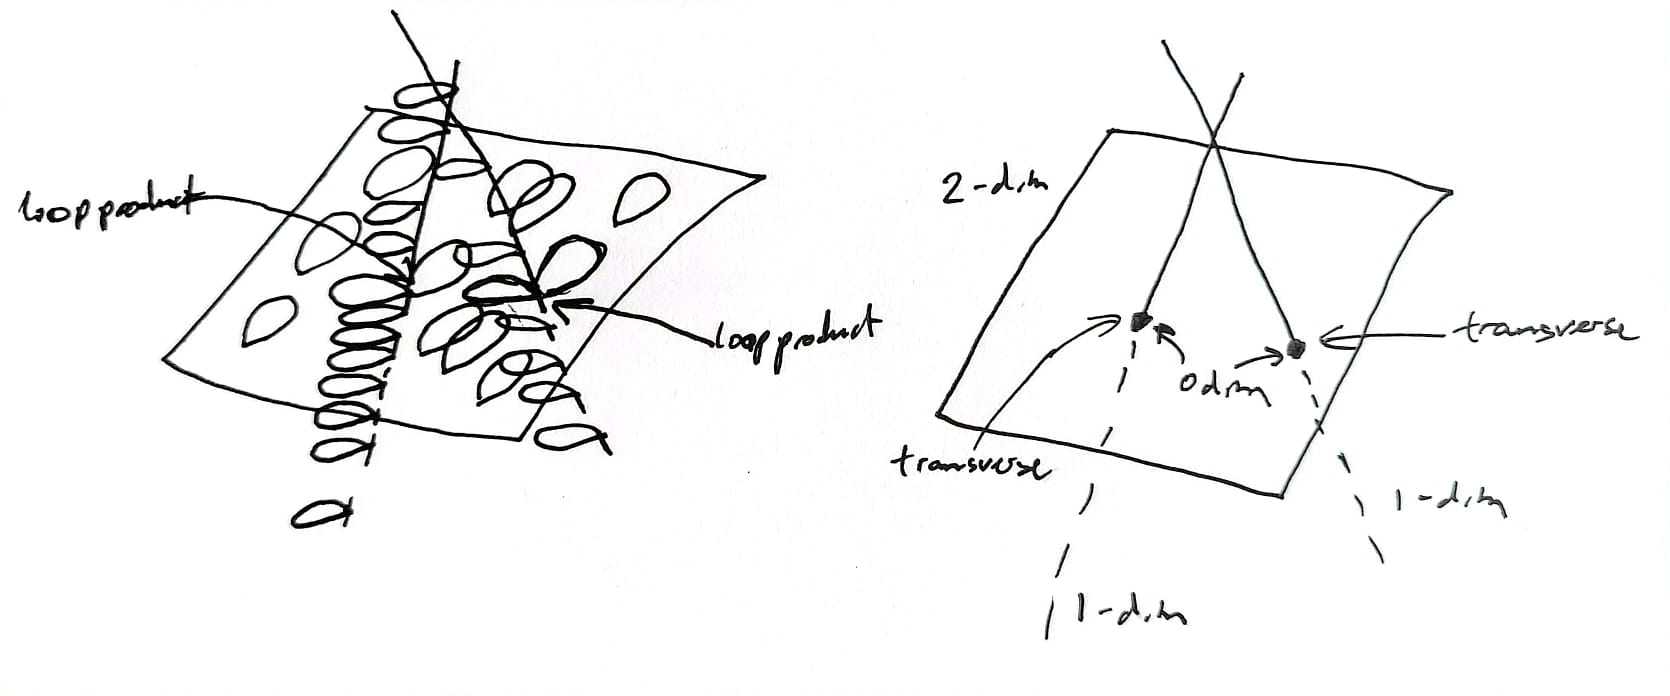
\includegraphics[width=0.9\textwidth]{Figures/DNOVXJ.jpeg}
    \caption{The transverse intersection of two $1$-chains and
    a $2$-chain in a $3$-manifold giving a $0$-chain as a 
loop product. \cite[From Figure 2]{Chas-Sullivan}}
    \label{fig:Figures-DNOVXJ-jpeg}
\end{figure}




\begin{definition}[Chas-Sullivan product $\wedge$]
    The \textit{Chas-Sullivan product} $\wedge$ is a lift
    of the intersection product making the following diagram commute:

    \begin{equation*}
    \begin{tikzcd}
        H_p(LM) \otimes H_q(LM) \ar[d, "\ev_0 \otimes \ev_0"] 
        \ar[r, "\wedge"] & H_{p+q-n}(LM) \ar[d, "\ev_0"] \\
        H_p(M) \otimes H_q(M) \ar[r, "\bullet"] &
        H_{p+q-n}(M)
    \end{tikzcd}
    \end{equation*}
\end{definition}

We now explain the construction.

Recall the $\varepsilon$-neighborhood $U_M$ of the diagonal
in $M \times M$ and now just pull this back along
$\ev_0 \times \ev_0$
 to $LM \times LM$ :
 \[
 U_{CS} = \left( \ev_0 \times \ev_0 \right)^{-1} U_M = 
 \left\{ \left( \gamma, \lambda \right) \in LM \times LM  \mid 
 \left| \gamma(0) - \lambda(0) \right| < \varepsilon \right\} .
 \] 
 Defining a retraction
 \[
 R_{CS} \colon U_{CS} \to LM \times_M LM = 
 \left\{ \left( \gamma, \lambda \right) \in LM \times LM  \mid 
 \gamma(0) = \lambda(0) \right\} = 
 \left( \ev_0 \times \ev_0 \right)^{-1} \left( \Delta_M \subset 
 M \times M \right) 
 \] 
 by concatenating with a "geodesic stick" to connect the loops
 so that they form a "figure 8":
 \[
 R_{CS}\left( \gamma, \lambda \right) = 
 \left( \gamma, \lambda' \right) \quad \text{with} \quad
 \lambda' = \overline{\gamma(0) \lambda(0)} \star \lambda
 \star \overline{\lambda(0) \gamma(0)}
 \] 
 where for $x,y \in M$ with $\left| x-y \right| < \rho$,
 $\overline{xy}$ denotes the unique minimal geodesic path
 $\left[ 0,1 \right] \to M$ from $x$ to $y$.
 Figure \ref{fig:Figures-HGFHEIA-png} describes this intuitively.

 \begin{figure}[htpb]
     \centering
     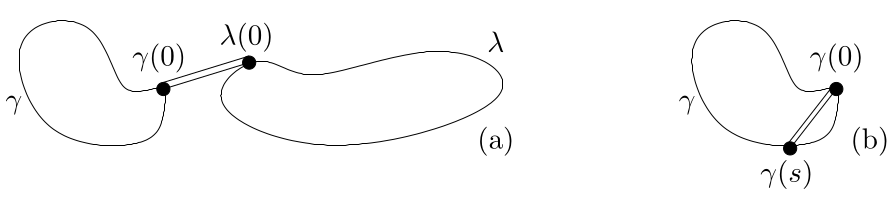
\includegraphics[width=0.8\textwidth]{Figures/HGFHEIA.png}
     \caption{Figures/HGFHEIA.png}
     \label{fig:Figures-HGFHEIA-png}
 \end{figure}

 This is a lift of the retraction $r \colon U_M \to M$ in the sense that

 \begin{equation*}
 \begin{tikzcd}
     U_{CS} \ar[d, "\ev_0 \times \ev_0"'] \ar[r, "R_{CS}"] & 
     LM \times_M LM \ar[d, "\ev_0"] \\
     U_M \ar[r, "r"] & M
 \end{tikzcd}
 \end{equation*}
 commutes.
 
 Pulling back $\tau_M$ along $\ev_0 \times \ev_0$ gives a cochain
 \[
 \tau_{CS} := \left( \ev_0 \times \ev_0 \right)^{*} \tau_M
 \in C^{*} \left( LM \times LM, LM \times LM - LM \times_M LM \right) 
 \] 
 
 Finally, we define the Chas-Sullivan loop product on chains as
 follows:

 \begin{definition}[Chas-Sullivan loop Product]
     The following sequence of chain maps induces the Chas-Sullivan
     product on homology:
     \begin{align*}
         \wedge \colon C_p (LM) \otimes C_{q} (LM) 
         \stackrel{\times }{\to} C_{p+q}(LM \times LM) 
         &\stackrel{\left[ \tau_{CS} \cap \right] }{\to} 
         C_{p+q-n}(U_{CS}) \\
         &\stackrel{R_{CS}}{\to} C_{p+q-n}\left( LM \times_M LM \right) 
         \stackrel{\text{concat}}{\to} C_{p+q-n}(LM).
     \end{align*}
 \end{definition}


 While this definition coincides with the Chas-Sullivan product
 in homology as described by
 Cohen-Jones, it is not necessarily clear how it coincides with the
 original geometric picture.
 However, Proposition \ref{Prop:GHUXIQL} guarantees tells us that it does.



 \subsubsection{Coproduct}
 
 Define
 $e_I \colon LM \times I \to M \times M$ by
 $e_I\left( \gamma, s \right) = \left( \gamma(0) , \gamma(s) \right) $.

 Set 
 \[
 U_{GH} = e_{I}^{-1} U_M = 
 \left\{ \left( \gamma, s \right) \in LM \times I  \mid 
 \left| \gamma(0) - \gamma(s) \right| < \varepsilon \right\} , 
 \] 
 and we have a commutative diagram
 \begin{equation*}
 \begin{tikzcd}
     U_{GH} \ar[r, "R_{GH}"] \ar[d, "e_I"] & 
     \mathcal{F} = \left\{ \left( \gamma, s \right) \in LM \times I  \mid 
 \gamma(0) = \gamma(s) \right\} \ar[r, hookrightarrow] 
 \ar[d, "e_I"] & LM \times I 
 \ar[d] \\
 U_M \ar[r, "r"] & \Delta M \ar[r, hookrightarrow] & 
 M \times M
 \end{tikzcd}
 \end{equation*}
 defining a retraction map
 $R_{GH}$ by concatenating with a geodesic stick to force self-intersection:

 \[
 R_{GH}(\gamma, s) = \left( \gamma', s \right) \quad
 \text{with} \quad
 \gamma' = \gamma \left[ 0,s \right] \star
 \overline{\gamma(s) \gamma(0)} \star_s 
 \overline{\gamma(0) \gamma(s)} \star
 \left[ s,0 \right] 
 \] 
 where the parametrization is chosen so that the concatenated loop
 passes through $\gamma(0)$ at time $s$; if $s = 0$ or $1$ as
 in the case $\gamma(0) = \gamma(s)$ to begin with, the
 geodesic sticks are of length $0$.

 \begin{definition}[Goresky-Hingston-Sullivan coproduct]
     The following sequence of chain maps is a chain model for
     the Goresky-Hingston-Sullivan coproduct:
     \begin{align*}
         \vee \colon 
         &C_p(LM,M) 
         \stackrel{\times I}{\longrightarrow} 
         C_{p+1}(LM \times I, LM \times \partial I \cup 
         M \times I) \stackrel{\left[ \tau_{GH} \cap \right] }{\longrightarrow} 
         C_{p+1-n}\left( U_{GH}, LM \times \partial I 
         \cup M \times I \right) \\
         &\stackrel{R_{GH}}{\longrightarrow} 
         C_{p+1-n}\left( \mathcal{F}, LM \times \partial I \cup 
         M \times I\right) \stackrel{cut}{\longrightarrow} 
         C_{p+q-n}\left( LM \times LM, M \times LM \cup 
         LM \times M \right) 
     \end{align*}
     This induces a well-defined degree $1-n$ map
     \[
     \vee \colon H_p (LM,M) \to 
     H_{p+1-n}\left( LM \times LM, M \times LM \cup 
     LM \times M \right) .
     \] 
 \end{definition}











\subsection{Computation via geometric intersection}

\begin{proposition}[]\cite[Propositions 3.1 and 3.7]{Hingston-Wahl}
    \label{Prop:GHUXIQL}
    \begin{enumerate}
        \item 
    If $Z_1 \colon \Sigma_1 \to LM$ and
    $Z_2 \colon \Sigma_2 \to LM$ are smooth cycles with the
    property that the maps
    $\ev_0 \circ Z_1 \colon \Sigma_1 \to M$ and
    $\ev_0 \circ Z_2 \colon \Sigma_2 \to M$ are transverse, then
    the loop product
    \[
    Z_1 \wedge Z_2 = \left( Z_1 \star Z_2 \right)|_{\Sigma_1 \times_{ev_0}
    \Sigma_2} \in H_* \left( LM \right) 
    \] 
    is the concatenation of the loops of $Z_1$ and $Z_2$ along
    the locus of the basepoint-intersections
    $\Sigma_1 \times_{\ev_0} \Sigma_2 \subset \Sigma_1 \times 
    \Sigma_2$, oriented as stated in \cite{Hingston-Wahl}
\item If $Z \colon \left( \Sigma, \Sigma_0 \right) \to 
    \left( LM, M \right) $ is a smooth relative cycle with the
    property that the restriction of $e_I \circ (Z \times I) \colon
    \Sigma \times I \to M \times M$ to $\left( \Sigma
    - \Sigma_0 \right) \times (0,1)$ is transverse to the diagonal,
    then
    \[
    \vee Z = \text{cut} \circ \left( Z \times I \right) 
    |_{\overline{\Sigma_{\Delta}}} \in H_* \left( LM \times 
    LM, M \times LM \cup  LM \times M \right) 
    \] 
    for $\overline{\Sigma_{\Delta}}$ the closure in
    $\Sigma \times I$ of the locus of basepoint self-intersecting
    loops $\Sigma_{\Delta} \subset \left( \Sigma - \Sigma_0 \right) 
    \times (0,1)$, oriented as stated in
    \cite{Hingston-Wahl}.
    \end{enumerate}
\end{proposition}

\begin{note}
    Here $\Sigma_1 \times_{\ev_0} \Sigma_2$ is the
    pullback

    \begin{equation*}
    \begin{tikzcd}
        \Sigma_1 \times_{\ev_0} \Sigma_2 \ar[r] \ar[d] & 
        \Sigma_2 \ar[d, "\ev_0 \circ Z_2"] \\
        \Sigma_1 \ar[r, "\ev_0 \circ Z_1"'] & M
    \end{tikzcd}
    \end{equation*}
    


\end{note}



\subsubsection{Lens spaces}

Consider $S^3 \subset \mathbb{C}^2$ as
$\left( r, \theta \right) = 
\left( \left( r_1, \theta_1 \right) , 
\left( r_2, \theta_2 \right) \right) $ with
$\theta_i \in \mathbb{R} / \mathbb{Z}$ and
$r_i \ge 0$, satisfying $r_1^2 + r_2^2 = 1$. Here
we think of
$S^3$ as
$\left\{ r_1 e^{i \theta_1} , r_2 e^{i \theta_2} \right\} $ with
$r_1^2 + r_2^2 = 1$.\\
In particular, when $r_i$ is zero, 
$\left( r_i, \theta_i \right) = 0$.\\
The lens
space $\mathcal{L}_{p,q} $, for $p,q$ coprime, is
the quotient space
$S^3 / \mathbb{Z}/p$ with the $\mathbb{Z}/p$ action defined by
\[
    \left( (r_1, \theta_1), (r_2 , \theta_2) \right) 
    \mapsto 
    \left( \left( r_1, \theta_1 + \frac{1}{p} \right) ,
    \left( r_2, \theta_2 + \frac{q}{p} \right) \right) .
\] 

There is a residual torus action on the lens space by
\begin{align*}
    \alpha \colon \left( S^{1} \times S^{1} \right) \times 
    \mathcal{L}_{p,q} 
    &\to \mathcal{L}_{p,q},\\
    \left( (s,t), (r,\theta) \right) 
    &\mapsto \left( \left( r_1, \theta_1 + \frac{s}{p} \right) ,
    \left( r_2, \theta_2 + \frac{s q}{p}+t \right) \right) 
\end{align*}


Using this residual torus action, we define cycles 
$Z_{l,m}$ for pairs of integers $(l,m)$ as follows:
let
\[
\delta_{l,m} \colon S^{1} \to S^{1} \times S^{1}
\] 
be the torus knot $t \mapsto \left( lt, mt \right) $ of
slope $\frac{l}{m}$. We can combine this loop with the
action $\alpha$ of the torus on $\mathcal{L}_{p,q}$ to get
a family
\begin{align*}
    Z_{l,m} \colon \mathcal{L}_{p,q} 
    &\to L \mathcal{L}_{p,q}\\
    \left( r,\theta \right) 
    &\mapsto 
    \left[ \gamma_{r,\theta}^{l,m} \colon
    t \mapsto \alpha \left( \delta_{l,m}(t), (r,\theta) \right) \right] 
\end{align*}
associated to each point $(r, \theta)$ in the lens space,
the loop $\gamma_{r,\theta}^{l,m}$ is based at this point
and follows the image of $\delta_{l,m}$ along the torus action.

That is, the loop is defined by
\[
\gamma_{r, \theta}^{l,m}(t) = 
\left( \left( r_1, \theta_1 + \frac{lt}{p} \right) ,
\left( r_2, \theta_2 + \frac{lt q}{p} + 
mt\right) \right) .
\] 
Note now that Lens spaces are manifolds, and
in particular, $\mathcal{L}_{p,q}$ are compact oriented
$3$-manifolds, so we can pick a fundamental class
$\left[ \mathcal{L}_{p,q} \right] $.\\
Denote by
\[
Z_{l,m} = 
\left( Z_{l,m} \right)_*
\left[ \mathcal{L}_{p,q} \right] \in H_3 \left( L \mathcal{L}_{p,q} \right) 
\] 
the associated homology class.
Suppose we now
postcompose with $\ev_0$, i.e.,
we look at the class
\[
    \left( \ev_0 \right)_*
    Z_{l,m} \in 
H_3 \left( \mathcal{L}_{p,q} \right) 
\] 
we note that
the composition
$\ev_0 \circ Z_{l,m}$ is just the 
identity,
so this just sends
$\left[ \mathcal{L}_{p,q} \right] $ to itself.
Thus also $Z_{l,m} \in 
H_3 \left( L \mathcal{L}_{p,q} \right) $ is non-trivial.\\
\linebreak

\subsubsection{The loop product of the classes
$Z_{l,m}$}

Let $Z_1 = Z_{l_1, m_1}$ and
$Z_2 = Z_{l_2, m_2}$.
Since $\ev_0 \circ Z_i$ is the identity for both $i$,
$\ev_0 \circ Z_1$ is transverse to
$\ev_0 \circ Z_2$.

Furthermore, the locus of basepoint-intersections
is the pullback
\begin{equation*}
\begin{tikzcd}
    \mathcal{L}_{p,q} \times_{\ev_0} 
    \mathcal{L}_{p,q} \ar[r] \ar[d] & \mathcal{L}_{p,q} \ar[d, "
    \ev_0 \circ Z_2"] \\
    \mathcal{L}_{p,q} \ar[r, "\ev_0 \circ Z_1"'] & \mathcal{L}_{p,q}
\end{tikzcd}
\end{equation*}
so
\begin{align*}
    \mathcal{L}_{p,q} \times_{\ev_0} \mathcal{L}_{p,q}
    &= \left\{ \left( \left( r_1,\theta_1 \right) ,
        \left( r_2, \theta_2 \right) \right)  \in \mathcal{L}_{p,q} \times 
    \mathcal{L}_{p,q}  \mid 
    (r_1,\theta_1) = \ev_0 Z_1 (r_1, \theta_1) = \ev_0 Z_2 (r_2, \theta_2)
    = \left( r_2, \theta_2 \right) 
\right\}\\
    &= \Delta \mathcal{L}_{p,q}
\end{align*}

Hence using Proposition \ref{Prop:GHUXIQL}, we obtain
that $Z_{l_1, m_1} \wedge
Z_{l_2, m_2}$ sends each point $\left( r, \theta \right) $
of $\mathcal{L}_{p,q} \cong \Delta
\mathcal{L}_{p,q}$ to the concatenated loop
$Z_{l_1,m_1} \star Z_{l_2,m_2}$ based at
$(r, \theta)$,
where $\star$ is the concatenation of the loops in the image
at their common basepoint.\\
\linebreak


We may as whether we can determined the loop product and
coproduct of these classes. Computations of both are carried
out in \ref{Naef-Rivera-Wahl} and we recount some of it here in
shorter form, following the source material closely.\\

Firstly, we turn to the product.

\begin{proposition}[]
    The Chas-Sullivan loop product of the classes
    $Z_{l,m} \in H_3 \left( L \mathcal{L}_{p,q} \right) $ defined
    above is given by summing the indices:
    \[
    Z_{l_1,m_1} \wedge Z_{l_2,m_2} = 
    Z_{l_1+l_2 , m_1+m_2}.
    \] 
\end{proposition}

\begin{proof}
    By the above considerations and
    Proposition \ref{Prop:GHUXIQL}, have
    \[
    Z_{l_1,m_1} \wedge
    Z_{l_2,m_2}  
    = \left( Z_{l_1,m_1}\star Z_{l_2,m_2} \right) |_{\Delta \mathcal{L}_{p,q}}
    \colon \mathcal{L}_{p,q} \cong
    \Delta \mathcal{L}_{p,q} \to L \mathcal{L}_{p,q}
    \] 
    where $\star$ is the concatenation of the loops in the image
    at their common basepoint, i.e.,
    it is the map
    $\mathcal{L}_{p,q} \to L \mathcal{L}_{p,q}$ sending
    $\left( r, \theta \right) \mapsto 
    \gamma_{r, \theta}^{l_1, m_1} * \gamma_{r, \theta}^{l_2, m_2}$ which
    is the image under the torus action of the
    concatenated loops
    $\left( l_1,m_1 \right) $ and $\left( l_2,m_2 \right) $ in the
    torus. Concatenation corresponds to addition
    in the fundamental group, so the
    concatenation becomes
    $\left( l_1,m_1 \right) * \left( l_2,m_2 \right) =
    \left( l_1+l_2, m_1+m_2 \right) $, so 
    $\gamma_{r,\theta}^{l_1,m_1} * \gamma_{r,\theta}^{l_2, m_2} =
    \gamma_{r, \theta}^{l_1+l_2, m_1+m_2}$.
    This homotopy descends to the lens space, so
    up to homotopy in the codomain,
    $Z_{l_1,m_1} \wedge Z_{l_2,m_2} = 
    Z_{l_1+l_2, m_1+m_2}$, and thus the classes
    agree in $H_{3} \left( L \mathcal{L}_{p,q} \right) $.
\end{proof}


Now that we have determined the loop product of the
classes, we turn to coproducts.

\subsubsection{$B$-classes}


Recall that the coproduct is a degree $1-3 = -2$ map on
$H_* (L \mathcal{L}_{p,q}, \mathcal{L}_{p,q})$:
\[
\vee \colon H_3 \left( L \mathcal{L}_{p,q}, \mathcal{L}_{p,q} \right) 
\to H_1 \left( L \mathcal{L}_{p,q} \times L \mathcal{L}_{p,q},
\mathcal{L}_{p,q} \times L \mathcal{L}_{p,q} \cup 
L \mathcal{L}_{p,q} \times \mathcal{L}_{p,q} \right) 
\] 

The coproduct of the classes
$Z_{l,m}$ will be given in terms of $B$-classes in the
target.


Let $\lambda \colon S^{1} \to \mathcal{L}_{p,q}$ be the
loop defined by $\lambda(t) = \left( (1, \frac{t}{p}),
0
\right) $ tracing the points $(r,\theta) \in \mathcal{L}_{p,q}$ 
with $\left( r_2, \theta_2 \right) = 0$. Then
$\lambda$ is a generator of
$\pi_1 \mathcal{L}_{p,q} \cong \mathbb{Z} / p$.

Note that
\[
    Z_{1,0}\left( (1,0), 0 \right) =
    \gamma_{\left( (1,0), 0 \right) }^{1,0} = 
    \left[ t \mapsto \left( (1, \frac{t}{p}), 0  \right)  \right] = 
    \lambda
\] 
Projecting a path
from $\left( \left( 1,0 \right) , 0 \right) $ to
$\left( 0, (1,0) \right) $ under
$Z_{1,0}$ gives a free homotopy
from
$\gamma_{\left( (1,0),0 \right) }^{1,0}$ to
$\gamma_{\left( 0, (1,0) \right) }^{1,0}$. Note that
\[
\gamma_{\left( 0, (1,0) \right) }^{1,0} = 
\left[ t \mapsto \left( 0, (1, \frac{qt}{p}) \right)  \right] 
= ( \lambda' )^{\star q}
\] 
for $\lambda' \colon S^{1} \to \mathcal{L}_{p,q}$ defined
by $\lambda' (t) = \left( 0, (1, \frac{t}{p}) \right) $.

\begin{definition}[]
    Define the $1$-cycles $B_{k,k'}$ and
    $B_{k,k'}'$ in
    $\mathcal{L}_{p,q}$ as follows:
    let $\lambda_s \colon S^{1} \to \mathcal{L}_{p,q}$ be the
    rotation of $\lambda$, based at $\lambda(s)$,:
    \[
    \lambda_s (t) = \lambda (s+t).
    \] 
    Similarly for $\lambda'$.
    Define
    \begin{align*}
        B_{k,k'} \colon S^{1} 
        &\to L \mathcal{L}_{p,q} \times_{\mathcal{L}_{p,q}}
        L \mathcal{L}_{p,q} \subset L \mathcal{L}_{p,q} \times 
        L \mathcal{L}_{p,q},\\
        s 
        &\mapsto \left( (\lambda_s)^{\star k},
        (\lambda_s)^{\star k' }\right) 
    \end{align*}
    We also denote by
    $B_{k,k'} \in H_1 \left( L \mathcal{L}_{p,q}
    \times_{\mathcal{L}_{p,q}} L \mathcal{L}_{p,q} \right) $ 
    or $H_1 \left( L \mathcal{L}_{p,q} \times L \mathcal{L}_{p,q} \right) $ 
    the associated homology class
    $\left( B_{k,k'} \right)_* \left[ S^{1} \right] $.
    Then the evaluation $\left( \ev_0 \right)_* \colon
    H_1 \left( L \mathcal{L}_{p,q} \times_{\mathcal{L}_{p,q}}
    L \mathcal{L}_{p,q}\right) \to 
    H_1 \left( \mathcal{L}_{p,q} \right) $ takes
     \[
     B_{k,k'} = \left( B_{k,k'} \right)_* \left[ S^{1} \right] 
     \mapsto \left( ev_0 \circ B_{k,k'} \right)_* \left[ S^{1} \right] 
     = \lambda_* \left[ S^{1} \right] = 
     \left[ \lambda \right] 
     \] 
     Define $B_{k,k'}'$ in the same way by
     replacing $\lambda$ by $\lambda'$ above.
\end{definition}




\begin{lemma}[]\cite[Lemma 2.6]{Naef-Rivera-Wahl}
    Let $B_{k,k'}' \colon S^{1} \to L \mathcal{L}_{p,q} \times_{
    \mathcal{L}_{p,q}} L \mathcal{L}_{p,q}$ be the family of
    figure eights based at the points of $\lambda'$ defined
    by $B_{k,k'}'(s) = 
    \left( (\lambda_s')^{\star k}, (\lambda_s')^{\star k'} \right) $. Then
    \[
    B_{k,k'} = q B_{qk,qk'}' \in 
    H_1 \left( L \mathcal{L}_{p,q} 
    \times_{\mathcal{L}_{p,q}} L \mathcal{L}_{p,q} \right) 
    \] 
    is the sum of $q$ copies of the class
    $B_{qk,qk'}'$.
\end{lemma}




\begin{lemma}[]\cite[Lemma 2.7]{Naef-Rivera-Wahl}
    We have that
    \begin{enumerate}
        \item $B_{k,k'} = B_{h,h'} \in 
            H_1 \left( L \mathcal{L}_{p,q} \times 
            L \mathcal{L}_{p,q} \right) $ if and only if
            $k = h \mod{p}$ and
            $k' = h' \mod{p}$.
        \item The relative classes
            \[
                \left\{ B_{k,k'} \right\}_{\substack{0 < k < p \\ 0 < k' <p}}
                \in H_1 \left( L \mathcal{L}_{p,q} \times 
                L \mathcal{L}_{p,q}, \mathcal{L}_{p,q}
            \times L \mathcal{L}_{p,q} \cup 
        L \mathcal{L}_{p,q} \times \mathcal{L}_{p,q} \right) 
            \] 
            are linearly independent over $\mathbb{Z}/p$.
    \end{enumerate}
\end{lemma}


\begin{proposition}[]\cite[Proposition 2.8]{Naef-Rivera-Wahl}
    The coproduct of the classes $Z_{l,m} \in H_3 \left( L \mathcal{L}_{p,q},
    \mathcal{L}_{p,q} \right) $ with $l,m \ge 0$ is given by
    the formula
    \[
    \vee Z_{l,m} = 
    \sum_{\substack{0 < k < l \\ k, (l-k) \neq 0 \mod{p}}}
    B_{k,l-k} + q' 
    \sum_{\substack{0 < k < ql+pm \\ k,(l-kq')\neq 0 \mod{p}}}
    B_{kq', l-kq'}
    \] 
    where $q'$ is the multiplicative inverse of $q \mod{p}$.
\end{proposition}

\begin{proof}

    We will only give the part of the proof that is necessary for
    us to understand the next section.\\
    \linebreak
    




    We want to make use of (2) in
    Proposition \ref{Prop:GHUXIQL}.

    To do this, we need $e_I \circ \left( Z \times I \right) 
    \colon \mathcal{L}_{p,q} \times I \to 
    \mathcal{L}_{p,q} \times \mathcal{L}_{p,q}$ 
    restricted to
    $(L \mathcal{L}_{p,q} - \mathcal{L}_{p,q}) \times (0,1) $
    to be transverse
    to the diagonal, where
    $e_I$ evaluates the loops at $0$ and
    $s \in \left( 0,1 \right)  \subset I$ (here
    $\mathcal{L}_{p,q} \subset L \mathcal{L}_{p,q}$ is the
    locus of constant loops).\\
    \linebreak
    Recall that
    $Z_{l,m}$ takes
    $\left( r, \theta \right) $ to
    $\left[ \gamma_{r,\theta}^{l,m} \colon
    t\mapsto \alpha \left( \delta_{l,m}(t), (r, \theta) \right) \right] $.
    If $(l,m)= (0,0)$, then $\delta_{0,0}$ is constant
    at $(0,0)$ and so
    $\alpha$ is constant at
    $\left( r, \theta \right) $, so $Z_{0,0}$ maps
    $(r, \theta)$ to the constant loop at $(r, \theta)$. Thus
    $Z_{0,0} = 0 \in H_3 \left( L \mathcal{L}_{p,q},
    \mathcal{L}_{p,q} \right) $.\\
    \linebreak
    Conversely, if
    $Z_{l,m}(r, \theta)$ is constant then
    $\left[ \gamma_{r, \theta}^{l,m} \colon
    t \mapsto 
\left( \left( r_1, \theta_1 + \frac{lt}{p} \right) ,
\left( r_2, \theta_2 + \frac{ltq}{p} +mt \right) \right) \right] $ 
    is constant at 
    $(r, \theta)$, so $l$ and $m$ must be $0$, hence
    if $(l,m) \neq (0,0)$, $Z_{l,m}$ has no constant
    cycles in its image.

    We can assume that $(l,m) \neq (0,0)$ and work
    with $\left( \Sigma , \Sigma_0 \right) = 
    \left( \mathcal{L}_{p,q}, \varnothing \right) $.

    \textit{Transversality:} represent the homology
    class of $Z_{l,m}$ by the homotopic family
    $\tilde{Z}_{l,m} \colon \mathcal{L}_{p,q} \to 
    L \mathcal{L}_{p,q}$ defined by
    $\tilde{Z}_{l,m}(r, \theta) = 
    \tilde{\gamma}_{r,\theta}^{l,m}$ for
    $\tilde{\gamma}_{r, \theta}^{l,m} \colon S^{1} \to 
    \mathcal{L}_{p,q}$  the loop based at 
    $(r , \theta)$ given by
    \[
    \tilde{\gamma}_{r, \theta}^{l,m} (t) = 
    \left( \left( \tilde{r}_{1}(t), \theta_1 + 
    \frac{lt}{p} \right), 
    \left( \tilde{r}_{2}(t), \theta_2 + \frac{ql+pm}{p}t \right) 
\right), 
    \] 
    where $\left( \tilde{r}_1(t), \tilde{r}_2(t) \right) $ is a
    deformation of $\left( r_1,r_2 \right) $ with
    $\left( \tilde{r}_1 (t) , \tilde{r}_2(t) \right) =
    \left( r_1,r_2 \right) $ only for $r_1 = 0$ or
    $r_2 = 0$, or when $t = 0$ or $1$.
    For example, 
    we can let
    \[
    \tilde{r}_1(t) = 
    \begin{cases}
        (1-2t) r_1 + 2t r_1^2,& t \in \left[ 0,\frac{1}{2} \right] \\
        r_1^2 (2-2t) + r_1 (2t-1),& t \in \left[ \frac{1}{2},1 \right] 
    \end{cases}
    \] 
    and $\tilde{r}_2(t) = 
    \sqrt{1 - \tilde{r}_1(t)^2} $.\\
    \linebreak

    We can visualize this as follows: 
    foliate $S^{4} \cong \mathbb{R}^3 \cup \left\{ \infty \right\} $ 
    by tori. Then for fixed radii, the
    angle coordinates trace out a torus.
    Then $\mathbb{Z}/p$ still acts on this torus, and 
    it is on this quotient torus, that
    $\gamma_{r, \theta}^{l,m}$ lives.
    So understanding self-intersections amounts to
    understanding self-intersections on this quotient torus of the
    torus knot one is interested in.

    For example, if
    $m = 0$, then for $l\ge 1$,
    $Z_{l,m}\left( r , \theta \right) $ has
    $l-1$ self-intersections.

    But for large $l$ and $m$, these loops will have many self-intersections.
    What $\tilde{Z}_{l,m}$ does is that
    it makes it so that, as we vary $t$, we also vary
    the radius such that only the torus knots
    corresponding to the endpoints
    live on the original torus knot corresponding to
    $Z_{l,m}$. See Figure \ref{fig:Figures-foliating-tori-jpg}


    \begin{figure}[htpb]
        \centering
        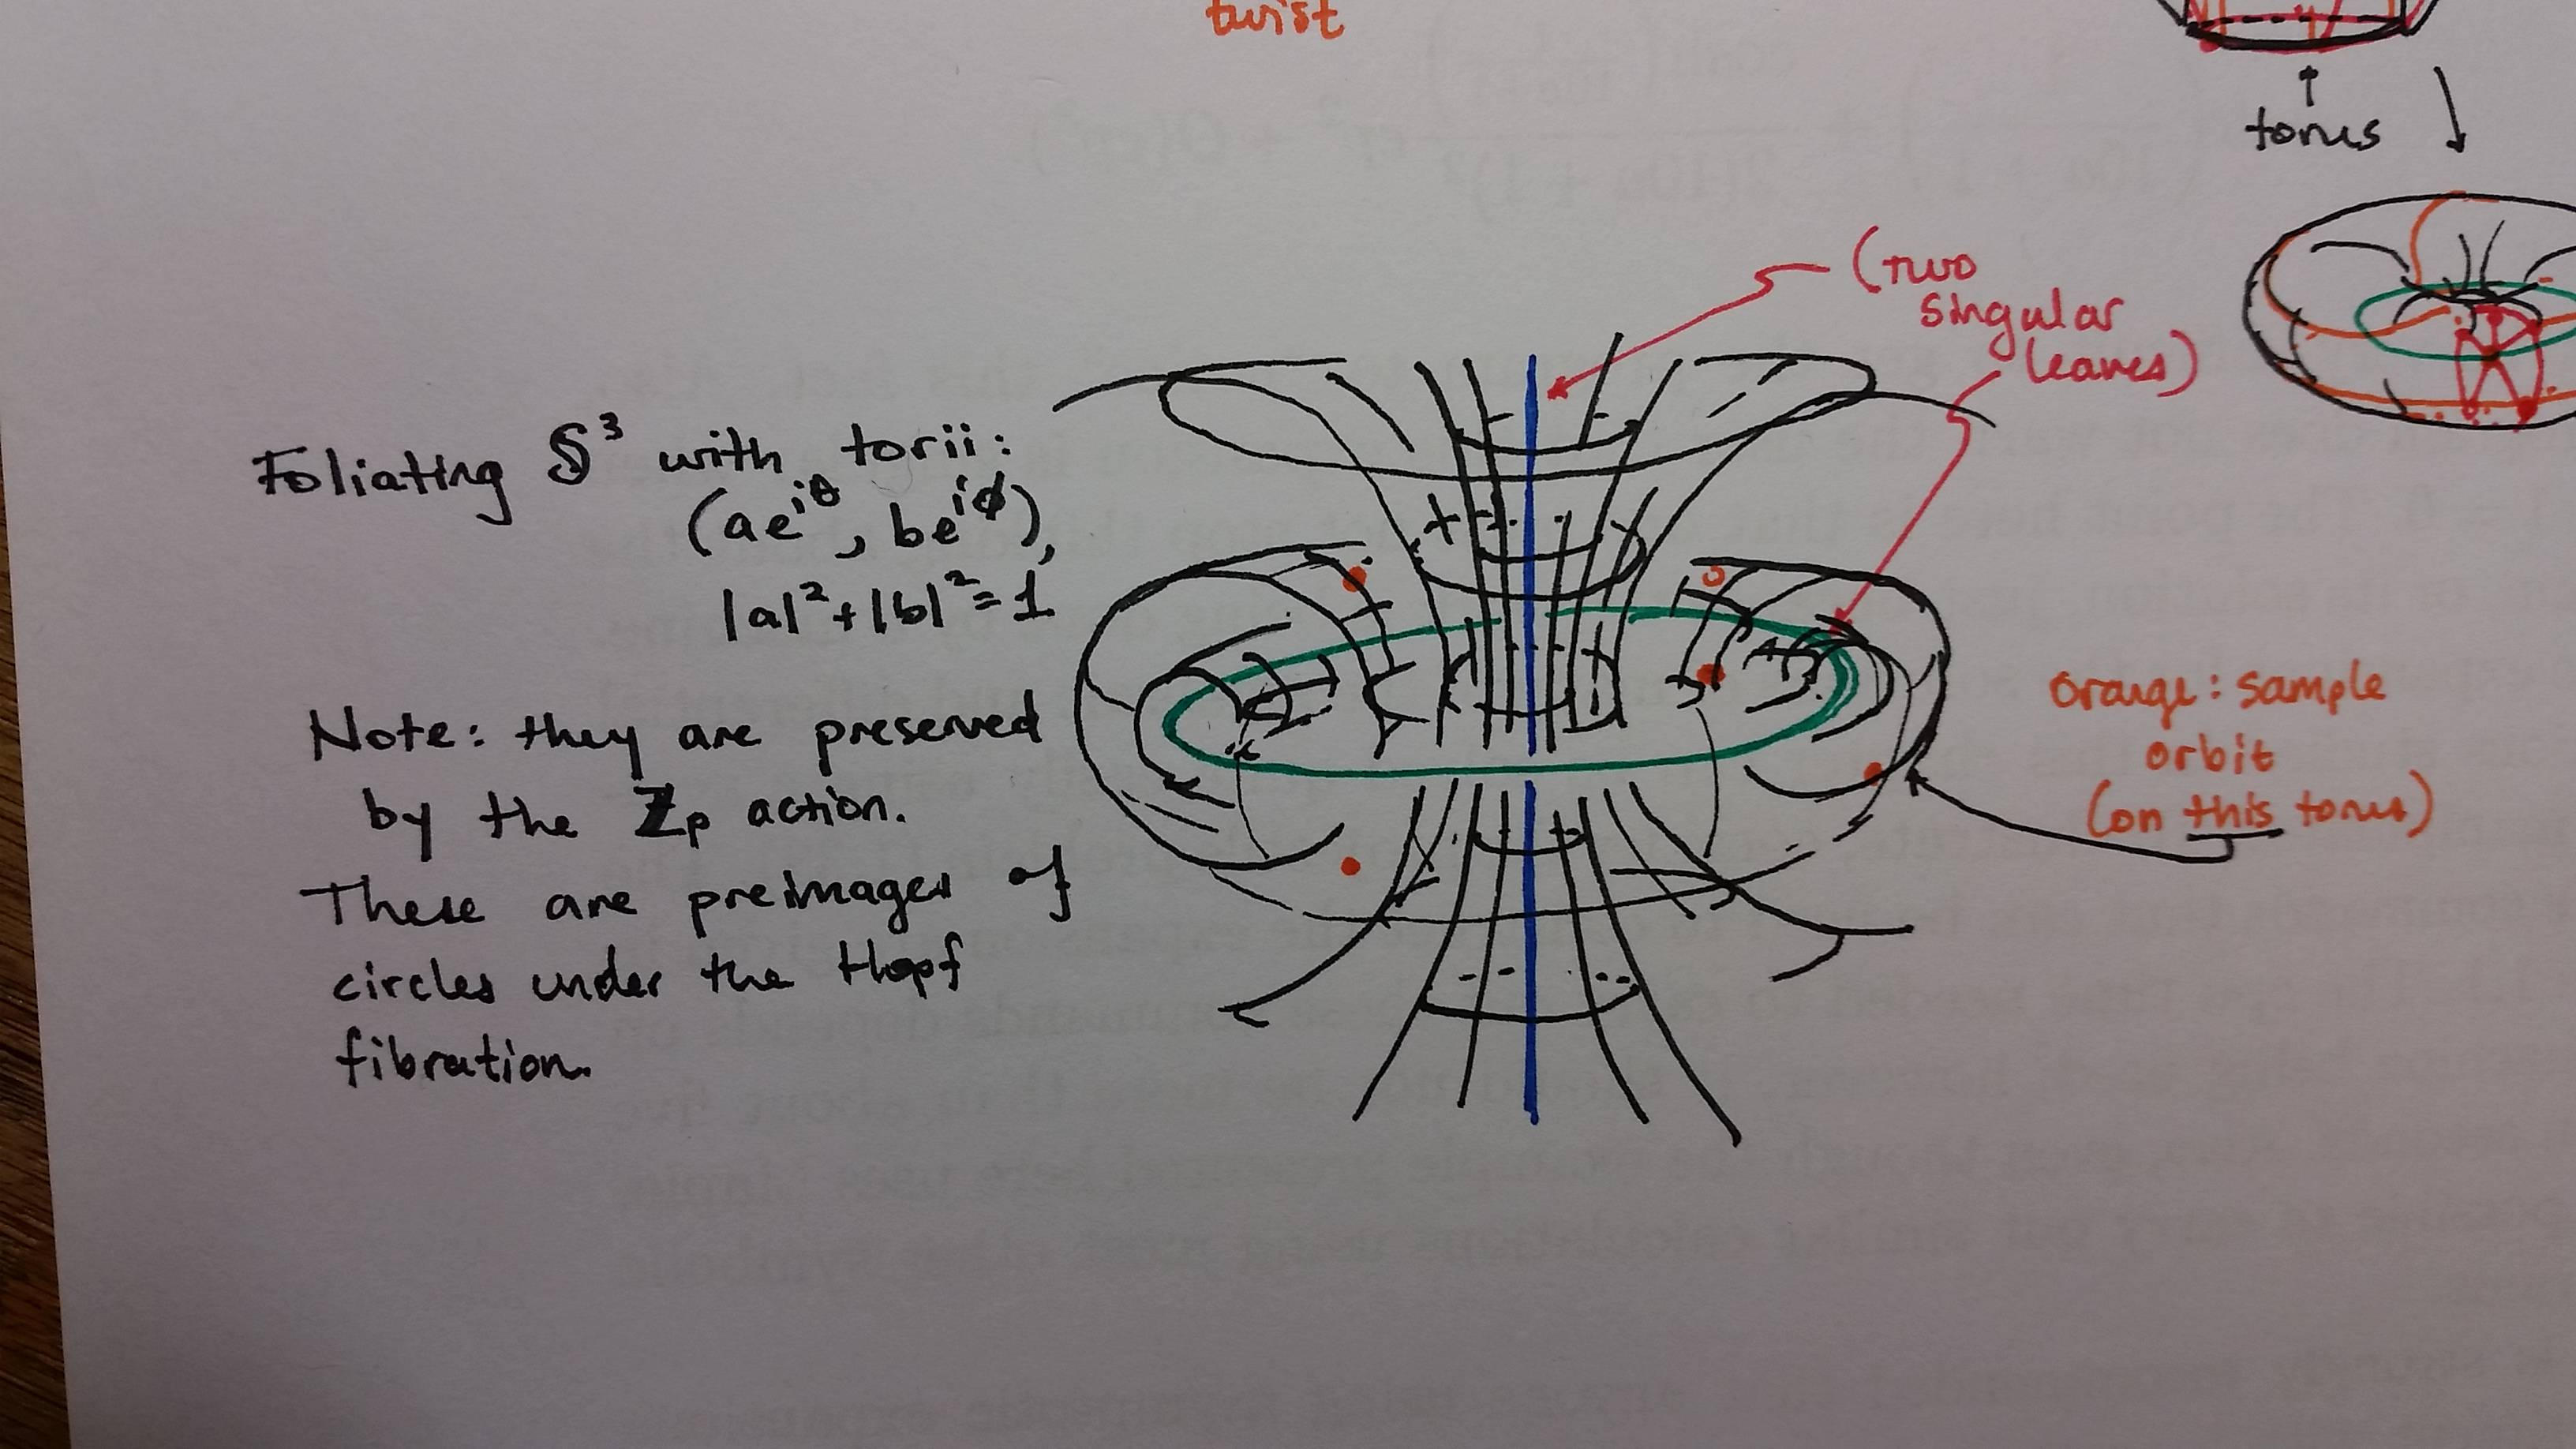
\includegraphics[width=1\textwidth]{Figures/foliating-tori.jpg}
        \caption{Figures/foliating-tori.jpg}
        \label{fig:Figures-foliating-tori-jpg}
    \end{figure}








    Then the map $e_I \circ \left( \tilde{Z}_{l,m}\times \id \right) 
    |_{\mathcal{L}_{p,q} \times  (0,1)}$ intersects
    the diagonal when $\tilde{\gamma}_{r,\theta}^{l,m}$ has a 
    self-intersection $\tilde{\gamma}_{r, \theta}^{l,m}(0)=
    \tilde{\gamma}_{r,\theta}^{l,m}(t)$ for
    some $t \in (0,1)$.


    Since the $r$ coordinates must match, such a self-intersection can
    only happen for $ r_1 = 0$
    or $r_2 = 0$ since otherwise
    $\tilde{r}_i(t) \neq \tilde{r}_i(0) = r_i$.

    For $r_2 = 0$, we have that
    $\tilde{r}_1(t) = r_1 = 1$ and
    $\tilde{r}_2 (t) = r_2 = 0$, and
    \[
    \tilde{\gamma}_{r, \theta}^{l,m} (t) = 
    \left( \left( 1, \theta_1 + \frac{lt}{p} \right) , 0 \right) 
    \] 
    The first angle coincides with
    $\theta_1$ precisely when
    $\frac{lt}{p} = \in \frac{1}{p}\mathbb{Z}$, i.e., when
    $t \in \frac{1}{l} \mathbb{Z} \cap (0,1)$.

    When $r_1 = 0$, we get
    \[
    \tilde{\gamma}_{r, \theta}^{l,m}(t) = 
    \left( 0, \left( 1, \theta_2 + \frac{ql+pm}{p}t \right)  \right) 
    \] 
    Since $\gcd (p,q) = 1$, Bezout gives that
    $ \frac{k}{p} = 0$ in the second coordinate, so 
     the second angle coincides with $\theta_2$ whenever
     $\frac{ql+pm}{p}t \in \frac{1}{p} \mathbb{Z}$.

     This yields the following parameters:

     \[
     \begin{cases}
         0 < t = \frac{a}{l} < 1, \text{ for some } a \in \mathbb{N} ,& 
         r_2 = 0\\
         0 < t = \frac{b}{ql+pm} < 1 \text{ for some } b \in \mathbb{N} ,&
         r_1 = 0.
     \end{cases}
     \] 
     So the locus of self-intersections of 
     $\tilde{Z}_{l,m} \times \id|_{\mathcal{L}_{p,q} \times (0,1)}$ is
     \[
     \Sigma_{\Delta} = 
     \left( \lambda \times I_1 \right) \cup 
     \left( \lambda'\times I_2 \right) \subset \mathcal{L}_{p,q} \times 
     (0,1)
     \] 
     where $I_1 = \left\{ \frac{1}{l}, \ldots,
     \frac{l-1}{l}\right\} $, 
     $I_2 = \left\{ \frac{1}{ql+pm}, \ldots, \frac{ql+pm-1}{ql+pm} \right\} $,
     and $\lambda, \lambda'$ are the loops parametrizing the
     points with $r_2 = 0$ and $r_1 = 0$, respectively.\\
     Note that $\lambda$ and $\lambda'$ correspond to the
     two degenerate cases of tori in the foliation.\\
     \linebreak
     The rest of the proof is a check of transversality at these
     points. We will skip this part and refer the reader to
     \cite{Naef-Rivera-Wahl}.






\end{proof}




\newpage

\subsection{Other potential operations}


Consider the $3$-simplex
$\Delta^3 = \left\{ \left( x_1,x_2,x_3 \right) \in \mathbb{R}^3  \mid 
0 \le x_1 \le x_2 \le x_3 \le 1\right\} $, and
consider the homology group

Since $\left( \Delta^3, \partial \Delta^3 \right) 
\cong \left( D^3, S^2 \right) $,
so
\[
H_3 \left( \Delta^3 / \partial \Delta^3 \right) \cong
H_3 \left( D^3, S^2 \right) \cong
\mathbb{Z}.
\] 
We want to see if we can construct an interesting
homomorphism
\[
H_3 \left( L \mathcal{L}_{p,q} \right) \to 
H_0 \left( L \mathcal{L}_{p,q} \right) 
\cong \mathbb{Z}^{p}
\] 

By the above, we can consider "products" of the form
\[
H_3 \left( L \mathcal{L}_{p,q} \right) \otimes
H_3 \left( \Delta^3 / \partial \Delta^3 \right) 
\to H_0 \left( L \mathcal{L}_{p,q} \right) 
\] 
or more generally,
\[
H_p \left( LM \right) \otimes
H_q \left( \Delta^3 / \partial \Delta^3 \right) \to 
H_{p+q-2n}\left( LM \right) 
\] 
which is only really interesting for
$q = 0,3$.\\
\linebreak




Let $E \colon
LM \times \Delta^3 / \partial \Delta^3 \to 
M^{4}$ be defined by
$E\left(\gamma, \left( x_1,x_2,x_3 \right)  \right) = 
\left( \gamma(0), \gamma(x_2), \gamma(x_1),
\gamma(x_3)\right)  $. Define
a map $\Delta \times \Delta\colon M^2 \hookrightarrow M^{4}$ by
$\Delta \times \Delta \left( m,n \right) = 
\left( m,m,n,n \right) $.
Form the pullback
\begin{equation*}
\begin{tikzcd}
    LM \times_{M^{4}} \Delta^3 / \partial \Delta^3
    \ar[r] \ar[d] & LM \times \Delta^3 / \partial \Delta^3
    \ar[d, "E"] \\
    M^2 \ar[r, "\Delta \times \Delta"] & M^{4}
\end{tikzcd}
\end{equation*}

This pullback consists of loops $\gamma$ for which
there exist some
$0 < x_1 < x_2 < x_3 < 1$ such that
$\gamma (0) = \gamma(x_2)$ and
$\gamma(x_1) = \gamma(x_3)$.

On this space, we define an operation

$\Upsilon \colon LM \times_{M^{4}} \Delta^3 / \partial \Delta^3 \to 
LM$ given by
concatinating the loop as shown in the figure

\begin{figure}[htpb]
    \centering
    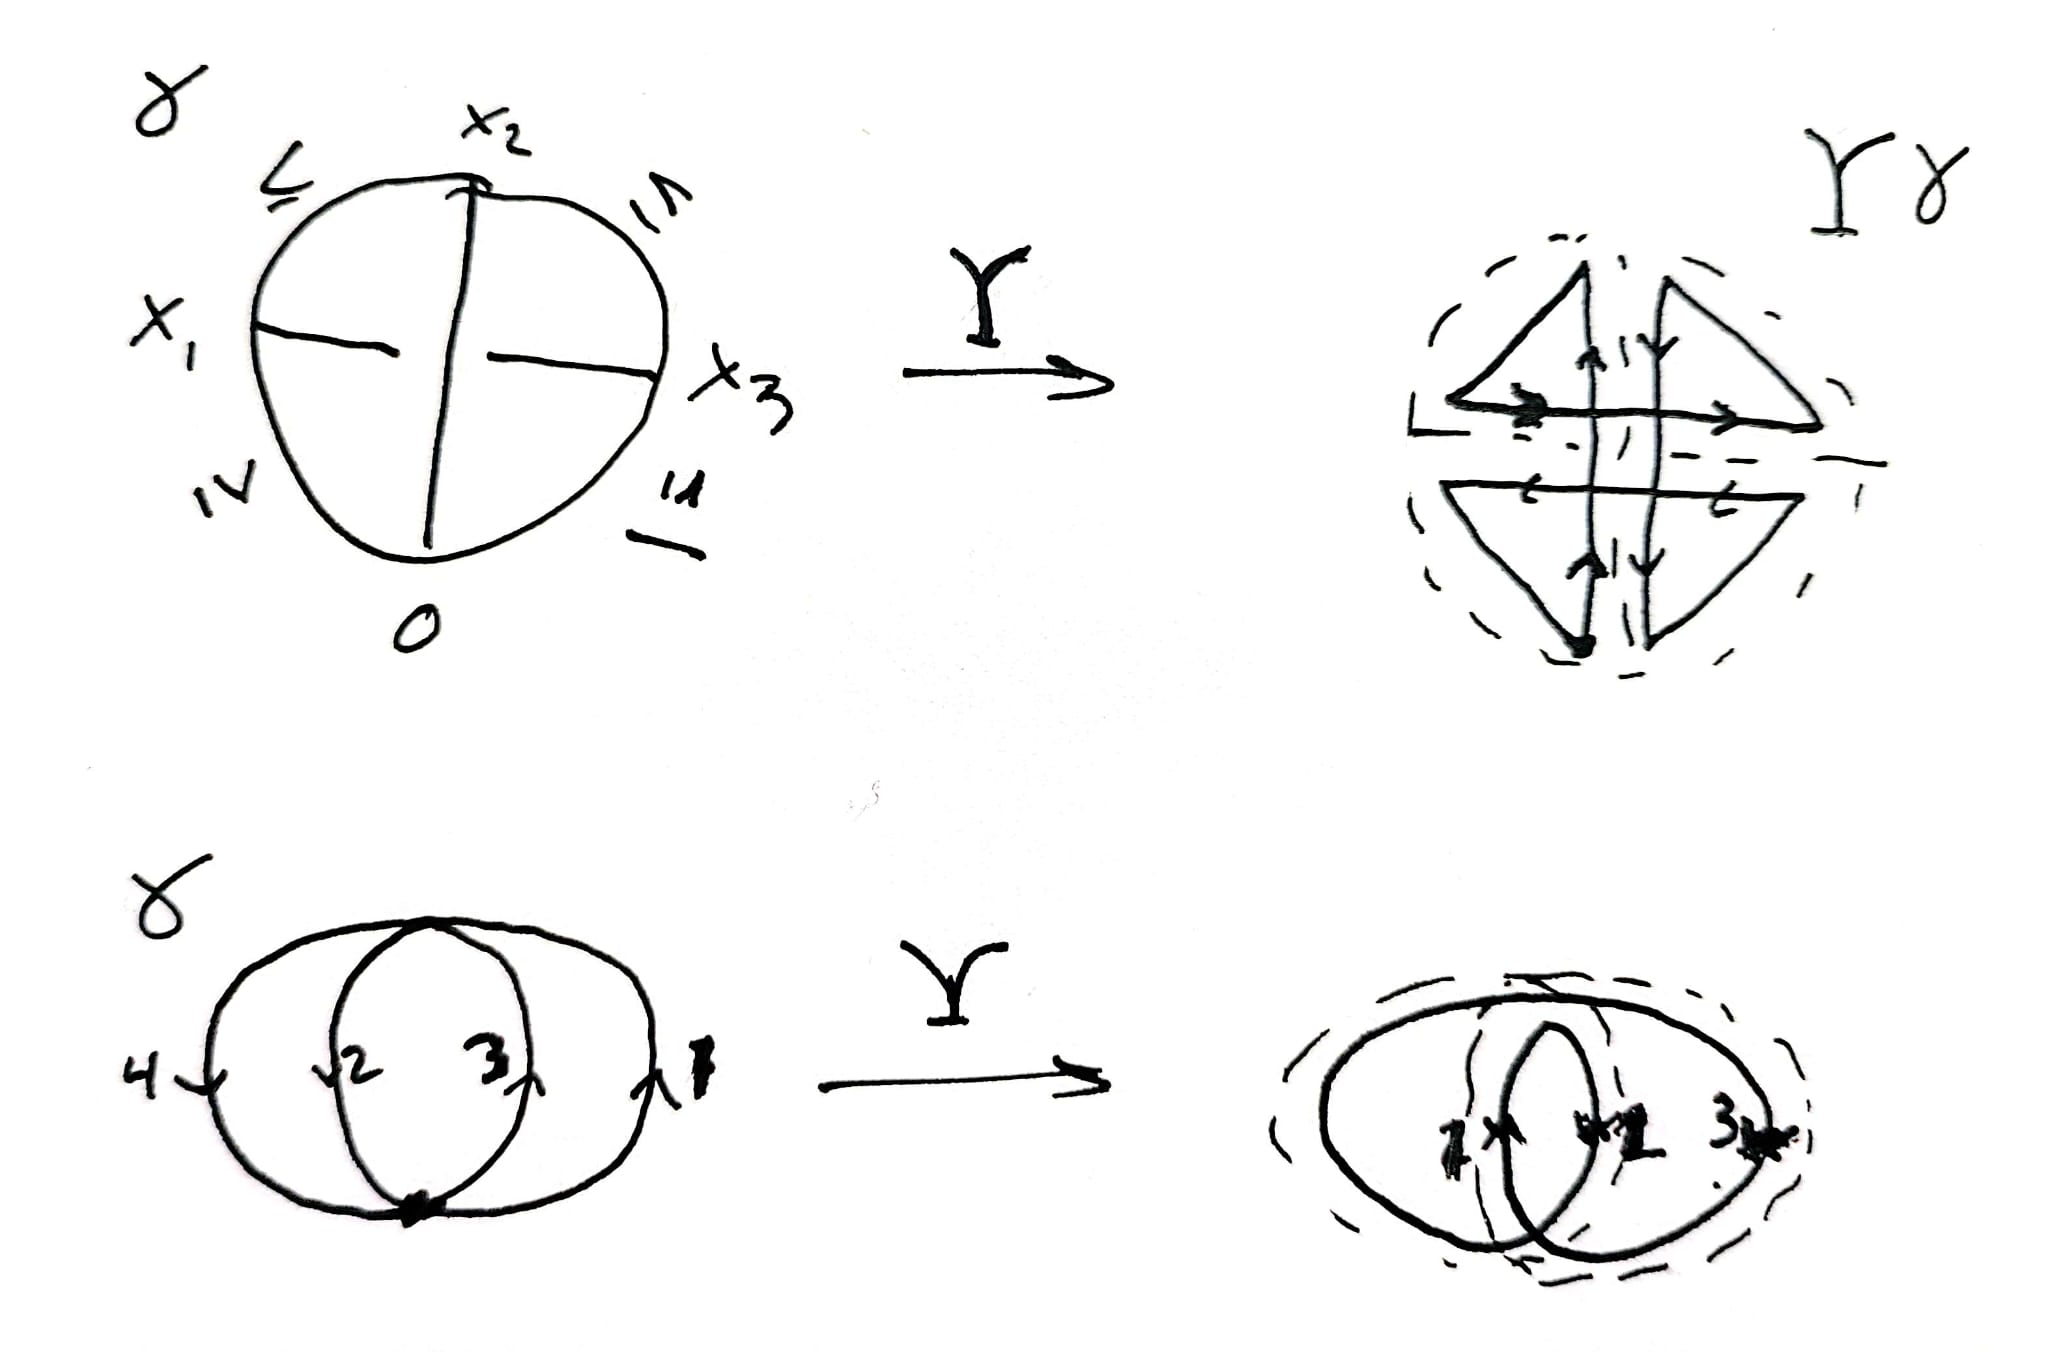
\includegraphics[width=0.8\textwidth]{Figures/UGWINZKQ.jpeg}
    \caption{$\Upsilon$ of a loop $\gamma$}
    \label{fig:Figures-UGWINZKQ-jpeg}
\end{figure}



(or $\Upsilon$ could potentially be some other operation).


Now similarly to the construction of the coproduct, we can define a map
$LM \times \Delta^{3} /\partial \Delta^3 \to LM \times_{M^{4}} \Delta^{3}
/ \partial \Delta^3$ by,
for an element
$\left( \gamma, \left( x_1,x_2,x_3 \right)  \right) $, inserting
a geodesic stick between $\gamma(0)$ and $\gamma(x_2)$ as well
as another geodesic stick between $\gamma(x_1)$ and 
$\gamma(x_3)$, and then forming the desired loop by concatinating
the different parts.


To make this precise, let us start by
considering the diagonal embedding
$\Delta \times \Delta \colon M \times M 
\hookrightarrow M^2 \times M^2$.
Its normal bundle is isomorphic to
the tangent bundle $T(M \times M) \cong TM \oplus TM$.
Again identify $T\left( M \times M \right) $ with
$T\left( M \times M \right)_{\varepsilon}$,
$\varepsilon \ll \rho$, $\rho$ the injectivity radius of $M \times M$.

Then the map
\[
\nu_{M \times M} \colon T\left( M \times M \right) 
\hookrightarrow M^{4} \quad
\nu_{M \times M}\left( \left( x,v \right) ,
\left( y,u \right) \right) =
\left( x, \exp_x v, y, \exp_y u \right) 
\] 
gives a tubular neighborhood
of $\Delta \times \Delta$, with image the
$\varepsilon$-image of the diagonal
\[
\nu_{M \times M} \colon T\left( M \times M \right) 
\stackrel{\cong}{\to} U_1 
= \left\{ \left( x,x',y,y' \right)  \mid 
\left| x-x' \right| , \left| y-y' \right| < \varepsilon \right\} 
\] 
and under this identification, the bundle projection
map $T\left( M \times M \right) \to M \times M$ becomes
the retraction
$r \colon U_1 \to M \times M$ by
$r\left( x,x',y,y' \right) = \left( x,y \right) $.

Let
$\tau_{M \times M}$ be the image of a cochain representative
for the Thom class for
$T\left( M \times M \right) $ under
the quasi-isomorphism
\[
C^{2n}\left( T(M \times M), T(M \times M) - M \times M \right) 
\stackrel{\simeq}{\to} 
C^{2n} \left( M^{4}, M^{4} - \Delta \times \Delta(M^2) \right) 
\] 

Now let

\[
    U_{2} = E^{-1}(U_1) = 
    \left\{ \left( \gamma, \left( x_1,x_2,x_3 \right)  \right)  \mid 
    \left| \gamma(0) - \gamma(x_2) \right| ,
    \left| \gamma(x_1)- \gamma(x_3) \right| < \varepsilon \right\} 
\]
and set
$\tau_{\Delta^3} = 
E^{*}(\tau_{M \times M})$.



On this neighborhood, we can concatenate with the desired geodesic sticks,
so we obtain a retraction
$R \colon U_2 \to LM \times_{M^{4}} \Delta^3 / \partial \Delta^3$ sending
\[
R (\gamma, \left( x_1,x_2,x_3 \right) )
= \left( \gamma', \left( x_1,x_2,x_3 \right)  \right) 
\] 
where $\gamma'$ is the desired loop
such that
the following diagram commutes:

\begin{equation*}
\begin{tikzcd}
    U_2 \ar[d, "E"] \ar[r, "R"] & LM \times_{M^{4}} \Delta^3 / \partial \Delta^3
    \ar[r, hookrightarrow] \ar[d, "E"] & LM \times \Delta^3 / 
    \partial \Delta^3 \ar[d, "E"] \\
    U_1 \ar[r, "r"] & \Delta (M \times M) \ar[r, hookrightarrow] & M^{4}
\end{tikzcd}
\end{equation*}


Now define the following operation composite:

\begin{align*}
    \wedge_{\Delta^3} \colon C_p(LM) \otimes 
    C_q(\Delta^{3} / \partial \Delta^3) \stackrel{\times }{\longrightarrow} 
    C_{p+q}\left( LM \times \Delta^3 / \partial \Delta^3 \right) 
    &\stackrel{\left[ \tau_{\Delta^3} \cap \right] }{\longrightarrow} 
    C_{p+q-2n} (U_2) \\
    &\stackrel{R}{\longrightarrow} C_{p+q-2n}
    \left( LM \times_M \Delta^3 / \partial \Delta^3 \right) 
    \stackrel{\Upsilon}{\longrightarrow} C_{p+q-2n}(LM).
\end{align*}

where the middle map
$\left[ \tau_{\Delta^3} \cap  \right] $ is defined as the composite

\begin{align*}
    \left[ \tau_{\Delta^3}\cap \right] 
    &\colon
C_{*}\left( LM \times \Delta^3 / \partial \Delta^3 \right) 
\to C_{*}\left( LM \times \Delta^3 / \partial \Delta^3 , LM \times \Delta^3 
    / \partial \Delta^3 - 
LM \times_M \Delta^3 / \partial \Delta^3 \right) \\
    &\stackrel{\sim}{\longrightarrow} 
C_* \left( U_2, U_2 - LM \times_M \Delta^3 / \partial \Delta^3 \right) 
         \stackrel{\tau_{\Delta^3} \cap}{\longrightarrow} 
        C_{* - 2n}\left( U_2 \right) 
\end{align*}

Note that for $A \in C_* \left( LM \times \Delta^3 / \partial \Delta^3
\right) $, $\left[ \tau_{\Delta^3} \cap \right] (A) = 
\tau_{\Delta^3} \cap \rho (A)$ where
$\rho \colon C_* \left( LM \times \Delta^3 / \partial \Delta^3 \right) 
\to C_* \left( LM \times \Delta^3 / \partial \Delta^3 \right) $ is a
chain map which subdivides simplices in such a way
that $\rho (A)$ is homologous to $A$ and every
simplex $\sigma$ in $\rho (A)$ has support
in either $U_2$ or $LM \times \Delta^3 / \partial \Delta^3 -
U_{2, \varepsilon_0}$, and hence
$\tau_{\Delta^3} \cap \rho (A)$ has support
in $U_{2}$.
Capping with the Thom class then kills all the simplices with support
in $LM \times \Delta^3 / \partial \Delta^3 - 
U_{2, \varepsilon_0}$ (Cf. \cite{Hingston-Wahl}).\\

Hence, for example, we obtain a product
\[
\wedge_{\Delta^3} \colon
H_{3}\left( L \mathcal{L}_{p,q} \right) 
\otimes H_3\left( \Delta^3 / \partial \Delta^3 \right) 
\cong H_3 \left( L \mathcal{L}_{p,q} \right) \to 
H_{0}\left( L \mathcal{L}_{p,q} \right) 
\cong \mathbb{Z}^{p}
\] 


\begin{question}
Consider now the classes
$Z_{l,m}$ from before.
One could ask what the operation $\Upsilon$ does to
$Z_{l,m}$ on points where it satisfies the desired condition.
\end{question}



Now, $Z_{l,m}$ maps $\left( r, \theta \right) $ to

\[
    \gamma_{r,\theta}^{l,m}(t) =
    \left( \left( r_1, \theta_1 + \frac{lt}{p} \right) ,
    \left( r_2, \theta_2 + \frac{ltq}{p}+mt \right) \right) .
\] 

Suppose we choose the points
$x_1, x_2,x_3$.

Since $Z_{l,m}(r , \theta)$ is contained in
a torus, our loops
$\Upsilon Z_{l,m}(r, \theta)$ will
be
$Z_{l,m}[x_2,x_1] \star Z_{l,m}[x_3, x_2] \star
Z_{l,m}[0, x_3] \star Z_{l,m}[x_1, 0]$.

Now, let $S^{1} \times S^{1} / \mathbb{Z}/p$ denote the torus quotiented
out by the action of $\mathbb{Z}/p$ on it.
Then we find that
\[
\pi_1 \left( S^{1} \times S^{1} / \mathbb{Z}/p \right) \cong
\left<a,b,c  \mid ab^{q} = c^{p} \right>^{ab}
\] 

So $Z_{l,m}(r, \theta)$ corresponds to
$c^{l} b^{m}$.

Now, in
$S^{1} \times S^{1} / \mathbb{Z}/p$, we can
take a path from $Z_{l,m}\left( r,\theta \right) (x_1) = 
Z_{l,m}\left( r, \theta \right) (x_3)$ to
$Z_{l,m}(r, \theta) (0)$ and we can homotope our
loop $Z_{l,m}\left( r ,\theta \right) $ such that
$Z_{l,m}\left( r, \theta \right) (0) = 
Z_{l,m}(r, \theta)(x_i)$ for $i = 1,2,3$.
See figure \ref{fig:Figures-NGIWKZN-jpeg}


\begin{figure}[htpb]
    \centering
    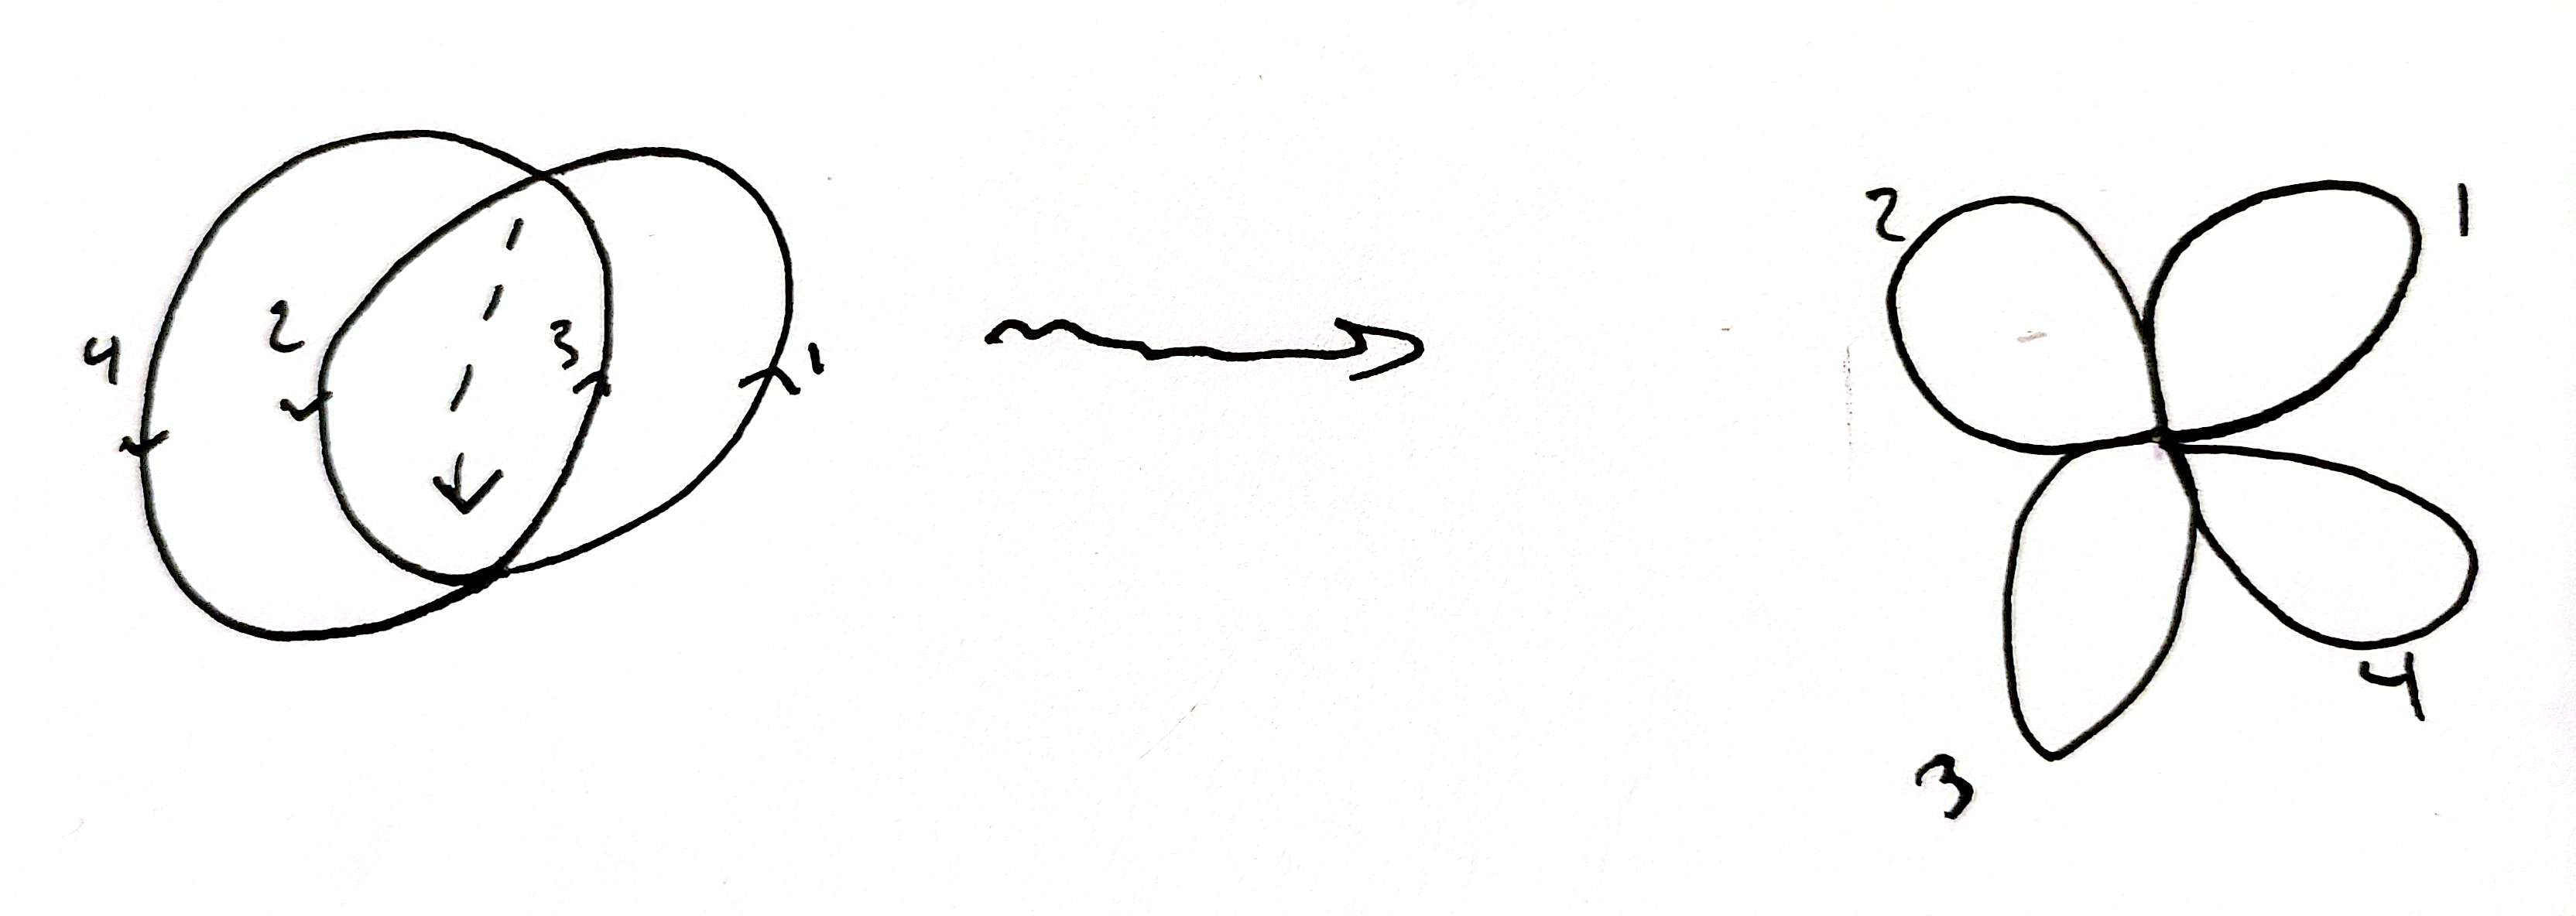
\includegraphics[width=0.7\textwidth]{Figures/NGIWKZN.jpeg}
    \caption{}
    \label{fig:Figures-NGIWKZN-jpeg}
\end{figure}


But in this loop, each of the segments
$Z_{l,m}[x_i, x_j]$ is a loop of its own, hence
lies in
$\pi_1\left( S^{1} \times S^{1} / \mathbb{Z}/p \right) $ which is
abelian, so in particular,
\begin{align*}
    \wedge_{\Delta^3} Z_{l,m}(r, \theta)
    &=
    Z_{l,m}[x_2,x_1] \star Z_{l,m}[x_3,x_2] 
    \star Z_{l,m}[0,x_3] \star
    Z_{l,m}[x_1,0]\\
    &\simeq 
    Z_{l,m}[0,x_3] \star Z_{l,m} [x_3, x_2] \star
    Z_{l,m}[x_2,x_1] \star Z_{l,m}[x_1,0]\\
    &=
    \overline{ Z_{l,m} (r , \theta)}
\end{align*}
where the bar denotes the inverse loop.

The question is whether this would also
work for other $\tilde{Z}_{l,m}$ for example. Does
it simplify to a simpler form?

We could likewise define other operations. For example, consider the
following operation
$\tilde{\Upsilon}$:

\begin{figure}[htpb]
    \centering
    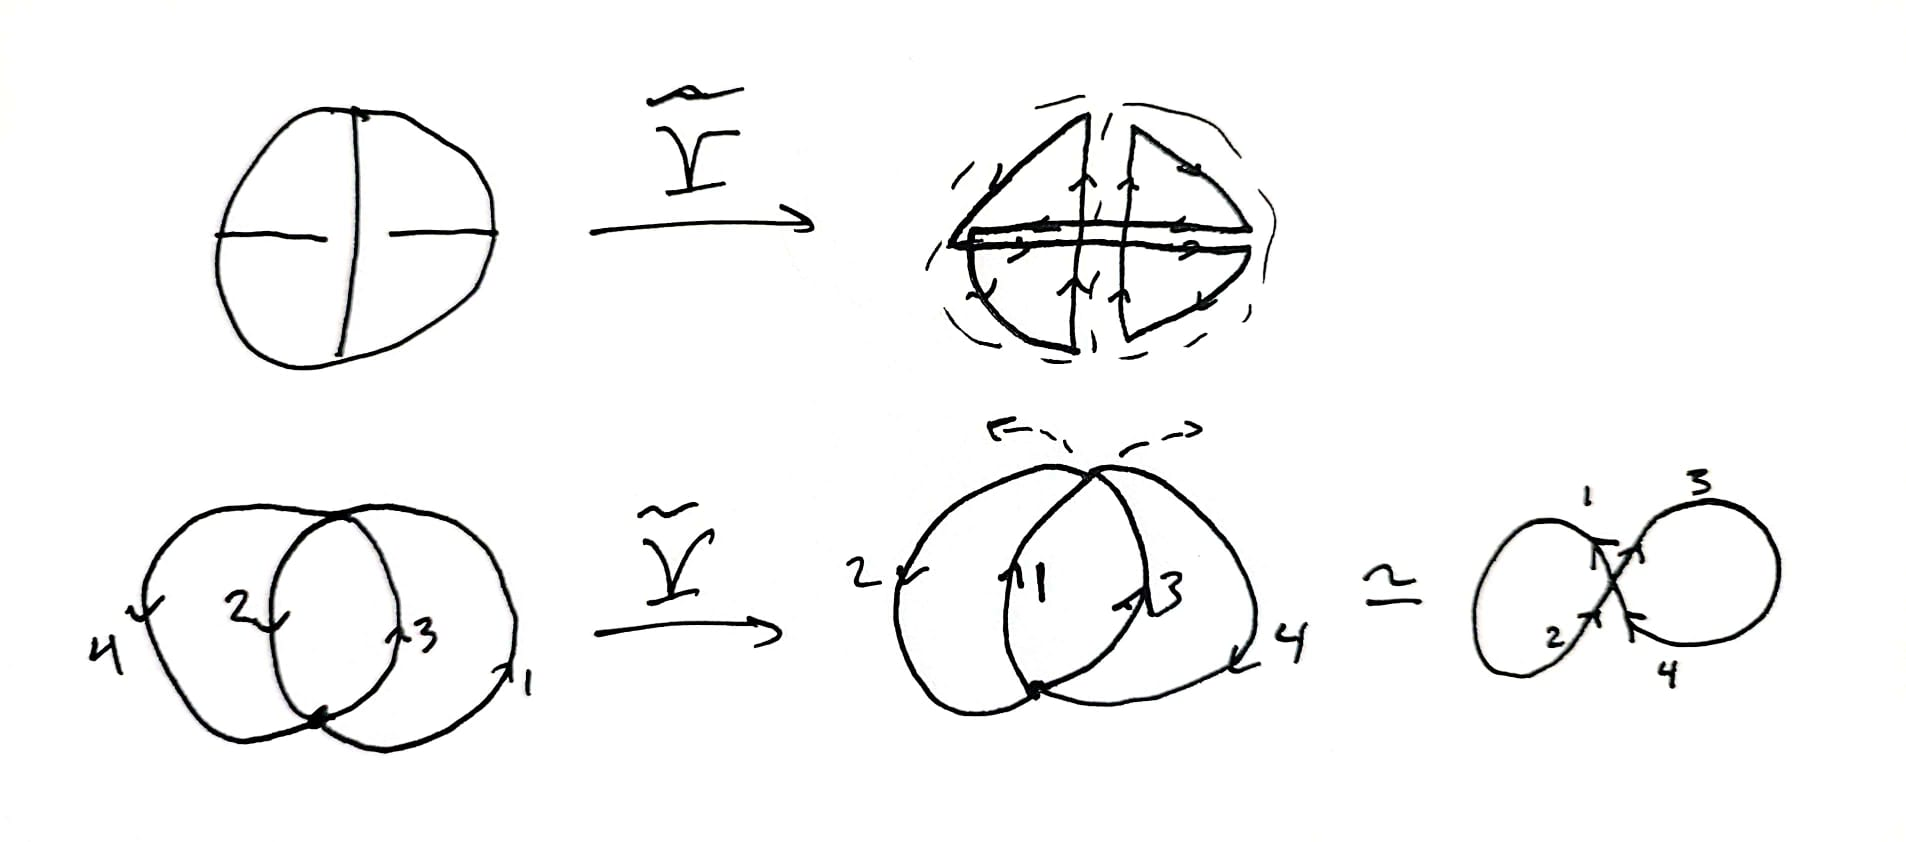
\includegraphics[width=0.8\textwidth]{Figures/NUIZKUW.jpeg}
    \caption{$\tilde{\Upsilon}$}
    \label{fig:Figures-NUIZKUW-jpeg}
\end{figure}

Using the same approach as before, this becomes
$\gamma \mapsto \gamma[x_2,0] \star \gamma[x_2, 1]$, i.e,
first half up to $x_2$ is $\gamma$ reversed up to
$x_2$, and the second part is $\gamma$ normally.\\
\linebreak


What does this do to a loop?\\
\linebreak


We now turn to a different question.


\begin{question}
    We have the following composition:

    \[
    C_{3}(\mathcal{L}_{p,q})
    \stackrel{Z_{l,m}}{\to} 
    C_3 \left( L \mathcal{L}_{p,q} \right) 
    \stackrel{\times \Delta^3 / \partial \Delta^3}{\to} 
    C_{6}\left( L \mathcal{L}_{p,q} \times 
    \Delta^3 / \partial \Delta^3 \right) 
    \stackrel{R \circ \left[ \tau_{\Delta^3}\cap \right] }{\to} 
    C_{0} \left( L \mathcal{L}_{p,q} \times_M 
    \Delta^3 / \partial \Delta^3 \right),
    \] 
    and we are interested in what the image of this composition is.
\end{question}

    By definition, it will be a finite sum
    of loops with marked points, $\left( \gamma, \left( x_1,x_2,x_3 \right) 
    \right) $, in
    $L \mathcal{L}_{p,q} \times_M \Delta^3 / \partial \Delta^3$ 
    with coefficients in $\mathbb{Z}$.

    Let us consider what this composition is doing.
    For some chain $\sigma$ in $\mathcal{L}_{p,q}$,
    we apply $Z_{l,m}$ to give a chain
    in $L \mathcal{L}_{p,q}$.
    Then we take the cross product with
    the quotient $3$-chain $\Delta^3 \to \Delta^3 / \partial \Delta^3$,
    which gives a $6$-chain in
    $L \mathcal{L}_{p,q} \times \Delta^3 / \partial \Delta^3$.
    Then $\left[ \tau_{\Delta^3} \cap \right] $ subdivides
    this chain until simplices
    are either in
    $U_2$ or its complement, but still remaining homologous
    to the original chain, and then we apply
    $\tau_{\Delta^3}$, which has support in $U_2$,
    essentially only leaves the chains contained in $U_2$.
     In $U_2$, we can apply
    $R$, and the resulting $0$-chain is the image.
    But furthermore, if
    the subdivided chain is transverse
    to $L \mathcal{L}_{p,q} \times_M \Delta^3 / \partial \Delta^3$, the by
    Corollary \ref{Cor:DNIZKJ}, capping with the Thom
    class will just give us the intersection of the chain with
    $L \mathcal{L}_{p,q} \times_M \Delta^3 / \partial \Delta^3$.

    So the problem reduces to 
    figuring out how to make $Z_{l,m} \times \Delta^3 / \partial \Delta^3$ 
    traverse to $L \mathcal{L}_{p,q} \times_M \Delta^3 / \partial \Delta^3$.
    But since we know that
    we must end in $C_0$ of the latter, we know that we must reduce
    to finite intersections.

    So let us start with the $\tilde{Z}_{l,m}$ from \cite{Naef-Rivera-Wahl}.

    Recall that its locus of self-intersection was
    \[
    \Sigma_{\Delta} = \left( \lambda \times I_1 \right) \cup 
    \left( \lambda' \times I_2 \right) \subset 
    \mathcal{L}_{p,q} \times (0,1)
    \] 
    where
    $I_1 = \left\{ \frac{1}{l},\ldots, \frac{l-1}{l} \right\} $ and
    $I_2 = \left\{ \frac{1}{pl+pm}, \ldots,
    \frac{ql+pm-1}{ql+pm}\right\} $, and
    $\lambda, \lambda'$ are the loops parametrizing the
    degenerate tori (circles) at the endpoints
    $r_2 = 0$ and $r_1 = 0$, respectively.
    

    For $0 < x_1 < x_2 < x_3 < 1$, if
    $\lambda(x_1 ) = \lambda(x_3)$, then
    $x_3 - x_1  \in  \frac{1}{l} \mathbb{Z}$.
    If $l>1$, there are infinitely many such pairs.
    
    For this, we must essentially break the periodicity in
    the angle coordinate.


    
    Let $g(t) = \sin\left( \alpha(l,m) t \right) -
    t \sin(\alpha(l,m))$.
    Consider the functions
    $\tilde{\theta}_1(t) =  
    \theta_1 + \frac{lt}{p}  + g(t)$ and
    $\tilde{\theta}_2 (t) = 
    \theta_2 + \frac{lqt}{p} + 
    g(t)$, and
    define $Z_{l,m}'(r, \theta) = 
    \gamma = 
    \left[ t\mapsto \left( \left( \tilde{r}_1(t), \tilde{\theta}_1 (t) \right) , 
    \left( \tilde{r}_2 (t) , \tilde{\theta}_2 (t) \right) \right) \right] $.
    For $Z_{l,m}'(r, \theta)$ to be in
    $L \mathcal{L}_{p,q} \times_{\mathcal{L}_{p,q}}
    \Delta^3 / \partial \Delta^3$, we would need
    for some $0 < x_1 < x_2 < x_3 < 1$ that
    $\gamma(x_1) = \gamma(x_3)$ and
    $\gamma(0) = \gamma(x_2)$. Just as before,
    we deduce that
    $r_1 = 0$ or $r_2 = 0$.
    Next if 
    $\gamma(x_1) = \gamma(x_3)$, we must have
    $g(x_1) - g(x_3) = 
    \frac{l}{p}(x_3- x_1)$ or
    $(\frac{lq}{p} + m)(x_3-x_1)$.

    If we simply choose $\alpha(l,m)$ to be small enough, we
    can guarantee that this never happens - for example
    looking at the functions' graphs.
    So $Z_{l,m}'$ can be made to not intersect
    $L \mathcal{L}_{p,q} \times_{\mathcal{L}_{p,q}} \Delta^3 / 
    \partial \Delta^3$.
    




    

































\newpage


\section{Terminology}\label{Section:Terminology}

\begin{definition}[Neighborhood retract]
    If $A \subset X$ and $A$ has a neighborhood in $X$ of
    which it is a retract, then $A$ is called
    a \textit{neighborhood retract} (in $X$ ).
\end{definition}

\begin{note}
    Saying that $A \hookrightarrow X$ is a cofibration
    is stronger than saying that $A$ is a neighborhood retract.
\end{note}



\begin{definition}[Exponential Map]
    Let $M$ be a smooth manifold and
    $p \in M$. One can define the notion of a straight line
    through the point $p$.

    Let $v \in T_pM$ be a tangent vector to the manifold
    at $p$. Then there is a unique geodesic 
    $\gamma_v \colon \left[ 0,1 \right] \to M$ satisfying
    $\gamma_v (0) = p$ with initial tangent vector
    $\gamma_v' (0) = v$.
    The corresponding \textit{exponential map} is defined
    by $\exp_p (v) = \gamma_v(1)$.
\end{definition}

\begin{definition}[Injectivity Radius]
      The injectivity
      radius of a Riemannian manifold at a point $p$
      is the supremum of
      all radii for which the exponential map
      at $p$ is a diffeomorphism onto its image.
\end{definition}



\section{Lemmas}

\begin{lemma}[]\label{Lemma:XIOOQLSJ}
    Let $\pi \colon W \to N$ be a covering map and
    $M$ a connected space. Suppose
    $f,g \colon M \to W$ are maps such that
    $\pi \circ f = \pi \circ g$ and that
    $f(x) = g(x)$ for some $x \in M$. Then
    $f = g$.
\end{lemma}

\begin{proof}
    Show that the set
    \[
    Z = \left\{ z \in M  \mid f(z) = g(z)\right\} 
    \] 
    is closed and open.
\end{proof}

\begin{lemma}[]\label{Lemma:Pullback-Of-Normal-Bundle}
    Suppose $A \subset Y$, and  $f \colon X \to Y$ is transverse to 
    $A$. Then we claim that
    $f^{*}\left( N_A Y \right) \cong 
    N_{f^{-1}A}(X)$. That is, the pullback of the normal bundle
    of $A$ in $Y$ is the normal bundle of the preimage of $A$ in $X$.
\end{lemma}

\begin{proof}
    We have an induced map pointwise
    \begin{equation*}
    \begin{tikzcd}
        T_x X \ar[r, "df"] \ar[d] & T_{f(x)}Y \ar[d] \\
        (N_{f^{-1}(A)}X)_x = 
        T_{x}X / T_{x}f^{-1}(A) \ar[r, "\overline{df}", dashed] &
        T_{f(x)}Y / T_{f(x)}A = (N_A Y)_{f(x)}
    \end{tikzcd}
    \end{equation*}
    defining
    $\overline{df} \colon N_{f^{-1}(A)}X \to 
    N_A Y$.
    We also have the bundle map
    $\pi \colon N_{f^{-1}}(A) X \to X$, thus inducing a map
    $\varphi \colon N_{f^{-1}}X \to 
    f^{*}N_A Y$ by $\varphi \left( x, \left[ v \right]  \right) 
    = \left( x , \overline{df}\left[ v \right]  \right) $.
    Now, $\overline{df}$ can be seen to be injective directly,
    and surjectivity of $\overline{df}$ follows
    from surjectivity of $df$ which follows
    directly from our assumption of transversality.
\end{proof}







\newpage
\printbibliography
\end{document}
